\chapter{Detección de biomarcadores en cáncer de hígado y colon-recto}

\section{Objetivos}

Hay dos objetivos principales:
\begin{enumerate}
	\item Describir las características clínicas de los pacientes de cáncer de hígado y colon-recto.
	\item Predecir en base a unos pocos genes si una persona padece o no cáncer de hígado o cáncer de colon-recto. En clasificación multiclase se predice además el diagnóstico primario de cáncer.
\end{enumerate}

\section{Fuente de datos}

La fuente de los datos es GDC (\textit{Genomic Data Commons}) Portal, una plataforma web sobre cáncer del Instituto Nacional del Cáncer de Estados Unidos (\textit{National Cancer Institute}) \cite{GDCPortal, NationalCancerInstitute}. GDC Portal fue desarrollado por el Instituto Nacional del Cáncer de Estados Unidos, la Universidad de Chicago, el Instituto de Ontario para la Investigación del Cáncer y la empresa \textit{Leidos Biomedical Research}. Su principal fortaleza reside en la integración y armonización de diversas fuentes heterogéneas, creando así un sistema de información amplio y robusto \cite{Grossman2016}. \\

\newpage
\begin{center}
	\textbf{Figura 5}. Diagrama de funcionalidad y utilidad de GDC. Extraído de Grossman et al. \cite{Grossman2016}.
\end{center}
\begin{center}
	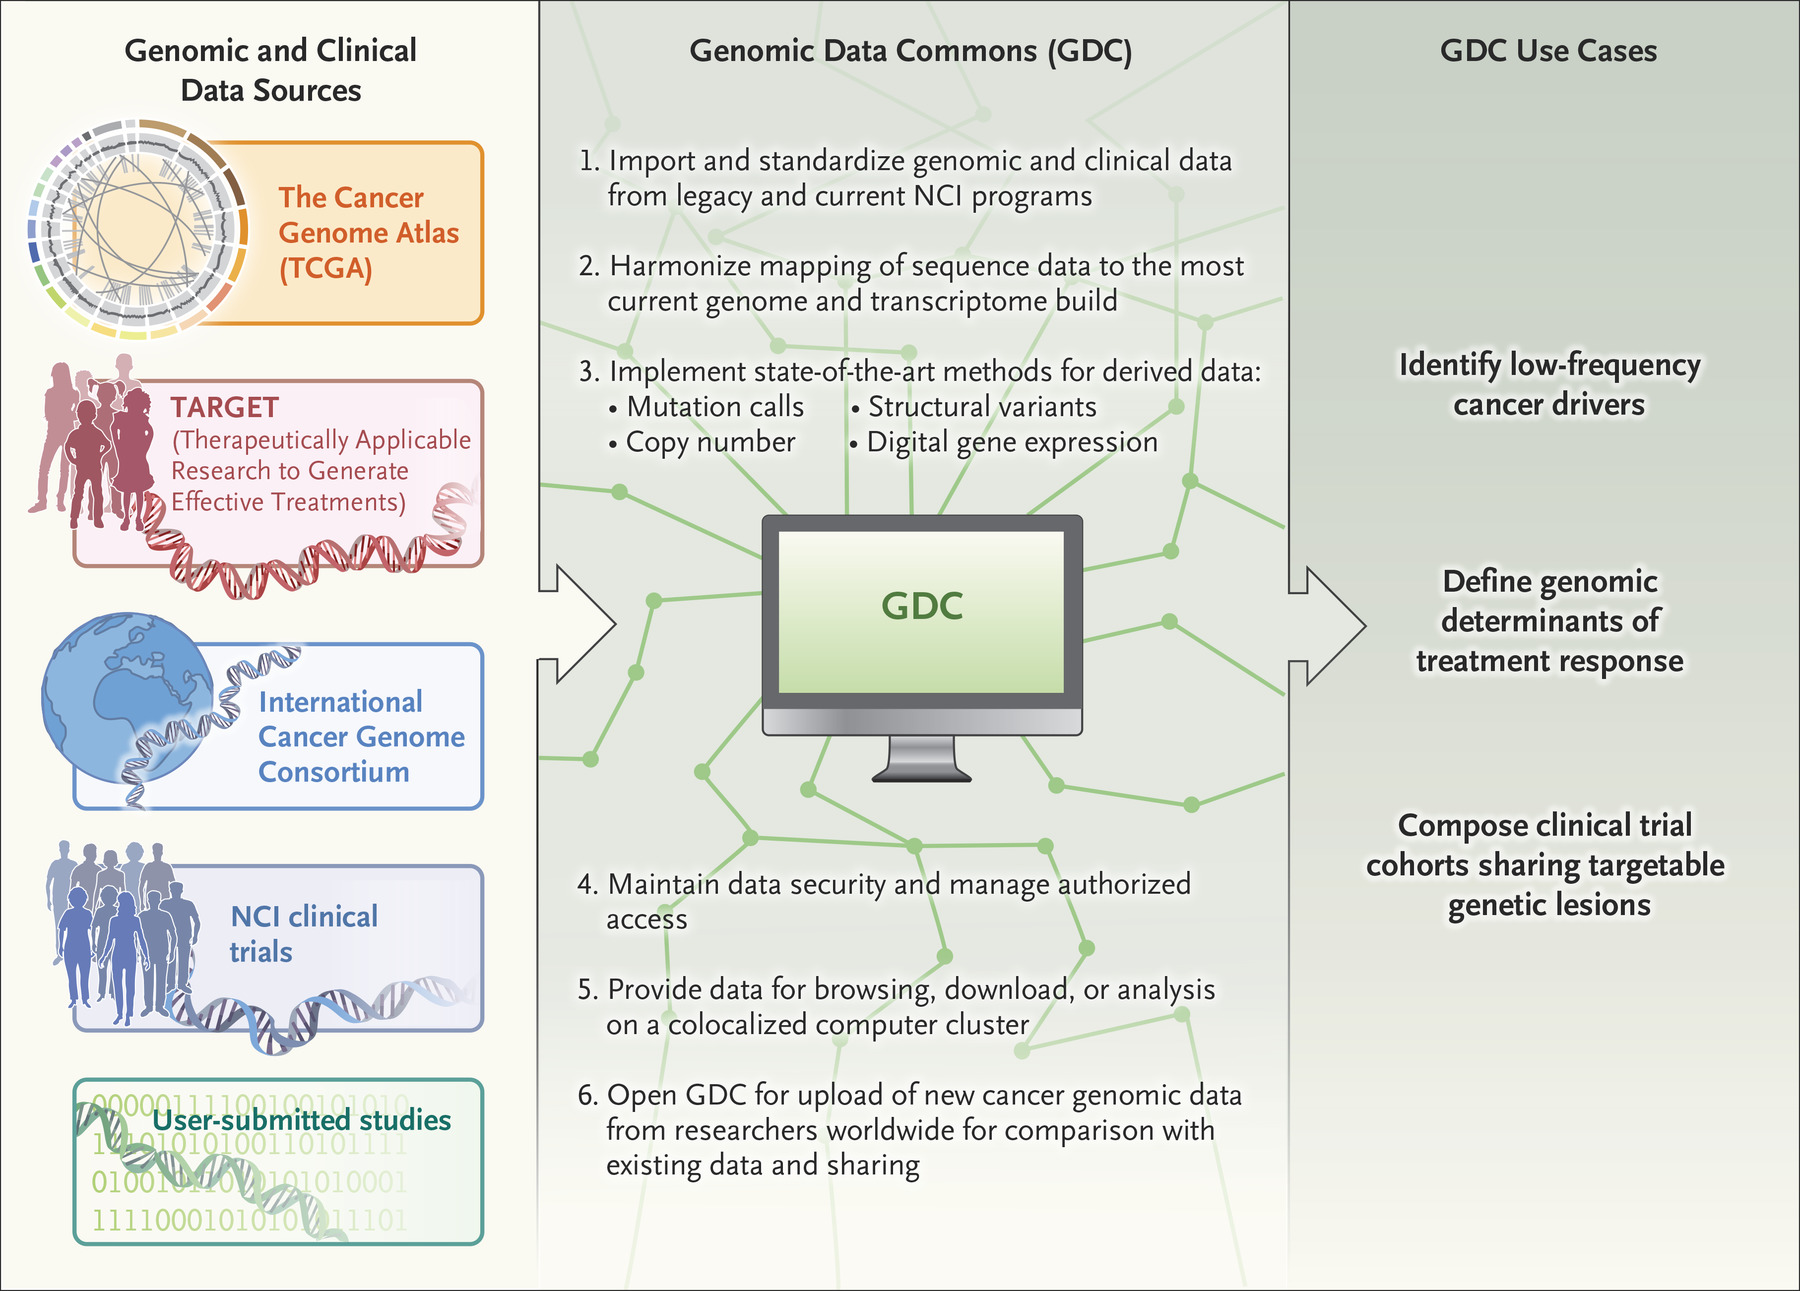
\includegraphics[width=1\textwidth]{figuras/05_funcionamiento_gdc.jpeg} 
\end{center}

A día 22 de Junio, GDC Portal contenía información sobre unos 84.000 casos, 23.000 genes y más de 3 millones de mutaciones de genes \cite{GDCPortal}. Algunos de estos datos son abiertos mientras que para otros es necesario solicitar acceso. La información de la que dispone es muy variada y se puede distinguir en tres grandes categorías:

\begin{itemize}
	\item Información clínica como la edad del sujeto, su sexo o el estadio del cáncer del que ha sido diagnosticado.
	\item Información genética y transcriptómica proveniente de diversos proyectos de investigación.
	\item Imágenes de tejidos tumorales y sanos.
\end{itemize} 

Para el presente trabajo se han descargado de GDC Portal todos los datos que cumplen las siguientes condiciones:

\begin{itemize}
	\item Son datos transcriptómicos del programa Cancer Genoma Atlas (TCGA), dirigido por dos organismos estadounidenses: el Instituto Nacional del Cáncer (NCI) y el Instituto Nacional para la Investigación del Genoma Humano (NHGRI) \cite{NationalCancerInstitutea}. 
	\item Contienen información sobre tumores o tejidos sanos de cáncer de hígado o colon-recto. Se han excluido metástasis y tumores recurrentes.
	\item El tipo de estrategia experimental es RNA-Seq y el tipo de flujo de trabajo es HTSeq - Counts. Esta información es de acceso abierto ya que no permite la identificación de un individuo.
\end{itemize}

Para cáncer de hígado se han descargado datos sobre 462 tejidos de los cuales 404 son cancerosos (87,4\%) y 58 son sanos (12,6\%).  Para cáncer de colon-recto se han descargado datos sobre 695 tejidos: 644 con cáncer (92,7\%) y 51 sanos (7,3\%). Es relevante destacar que las muestras de tejido sano se corresponden a tejido adyacente al tumor no afectado por el cáncer que es extraído del mismo paciente. Como no a todos los pacientes con cáncer se les ha secuenciado también tejido sano, existe un gran desequilibrio entre el número de muestras de las dos principales clases del problema.

\section{Características clínicas de los tumores}
 
A continuación se describe la información clínica de aquellas personas diagnosticadas con cáncer, descargada de la plataforma GDC Portal \cite{GDCPortal}. 

\subsection{Características clínicas para cáncer de hígado}

En la Tabla 9 se muestra  la distribución de casos de cáncer de hígado según algunas variables clínicas de interés. Los casos se recogieron entre los años 1995 y 2013, con el 67,6\% de los casos recogidos entre los años 2010 y 2013. La mayoría de los casos son hombres (65,3\%), están diagnosticados en estadios iniciales (70,3\% en estadios I y II) y son carcinomas hepatocelulares (89,6\%). La edad media de diagnóstico es de 60,1 años (mediana: 61,7 años) con un rango de edad que comprende de los 16 a los 87 años. Más de la mitad de los casos son caucásicos (52,5\%), que es la raza más común seguida por asiáticos (39,9\%) y afroamericanos (4,7\%). Aproximadamente dos de cada tres personas estaban vivas en el momento del último contacto realizado (63,6\%).

\newpage
\textbf{Tabla 9}. Características clínicas de los casos de cáncer de hígado. Distribución de casos y porcentaje según sexo, grupo de edad, raza, diagnóstico primario, estadio y estado vital.
\begin{table}[H]
	\centering \small
	\begin{tabular}{rrr}
		\hline
		\multicolumn{1}{l}{}                              & \textbf{Número de casos} & \textbf{Porcentaje}       \\ \hline
		\multicolumn{1}{l}{\textbf{Total}}                & 404                      & \multicolumn{1}{r}{100\%} \\ \hline
		\multicolumn{1}{l}{\textbf{Sexo}}                 &                          & \multicolumn{1}{l}{}      \\
		Hombre                                            & 264                      & 65,3\%                    \\
		Mujer                                             & 140                      & 34,7\%                    \\ \hline
		\multicolumn{1}{l}{\textbf{Grupo de edad}}        &                          &                           \\
		$\leq$ 40 años                                         & 34                       & 8,4\%                     \\
		41-50 años                                        & 40                       & 9,9\%                     \\
		51-60 años                                        & 106                      & 26,2\%                    \\
		61-70 años                                        & 127                      & 31,4\%                    \\
		71-80 años                                        & 77                       & 19,1\%                    \\
		$>$ 80 años                                     & 16                       & 4,0\%                       \\
		Desconocido                                       & 4                        & 1,0\%                       \\ \hline
		\multicolumn{1}{l}{\textbf{Raza}}                 &                          &                           \\
		Caucásico                                            & 212                      & 52,5\%                    \\
		Asiático                                          & 161                      & 39,9\%                    \\
		Afroamericano                             & 19                       & 4,7\%                     \\
		Desconocido                                       & 10                       & 2,5\%                     \\
		Indio americano o nativo de Alaska                & 2                        & 0,5\%                     \\ \hline
		\multicolumn{1}{l}{\textbf{Diagnóstico primario}} &                          &                           \\
		Carcinoma hepatocelular                           & 362                      & 89,6\%                    \\
		Colangiocarcinoma                                 & 33                       & 8,2\%                     \\
		Otros                                             & 8                        & 2,0\%                       \\ \hline
		\multicolumn{1}{l}{\textbf{Estadio}}              &                          &                           \\
		Estadio I                                         & 189                      & 46,8\%                    \\
		Estadio II                                        & 95                       & 23,5\%                    \\
		Estadio III                                       & 82                       & 20,3\%                    \\
		Estadio IV                                        & 7                        & 1,7\%                     \\
		Desconocido                                       & 31                       & 7,7\%                     \\ \hline
		\multicolumn{1}{l}{\textbf{Estado vital}}         &                          &                           \\
		Vivo                                              & 257                      & 63,6\%                    \\
		Fallecido                                         & 146                      & 36,1\%                    \\
		Desconocido                                       & 1                        & 0,2\%                     \\ \hline
	\end{tabular}
\end{table}

En la Tabla 10 se muestran tablas de contingencia del estado vital según sexo, grupo de edad y estadio. Se han realizado pruebas de chi cuadrado ($\chi^2$) \cite{Pearson1900} para evaluar la independencia o no del estado vital con respecto a las distintas variables, aplicando la corrección de Yates \cite{Yates1934} cuando fue necesario.\\

El código completo del análisis se muestra en el fichero \textit{\texttt{analisis\_higado/\linebreak01\_analisis\_datos\_clinicos.R}} del repositorio de GitHub asociado al trabajo \cite{Redondo-Sanchez2020}.\\

\textbf{Tabla 10}. Características clínicas de los casos de cáncer de hígado. Distribución de  estado vital según sexo, grupo de edad, estadio y diagnóstico primario.

\begin{table}[H]
	\centering
	\begin{tabular}{rccc}
		\cline{2-4}
		\multicolumn{1}{l}{}                              & \textbf{Vivos} & \textbf{Fallecidos} & \textbf{p-valor}     \\ \hline
		\multicolumn{1}{l}{\textbf{Número de tumores}}    & 257            & 146                 & \multicolumn{1}{l}{} \\ \hline
		\multicolumn{1}{l}{\textbf{Sexo}}                 &                &                     & 0,033                \\
		Hombre                                            & 178 (67,7\%)   & 85 (32,3\%)         &                      \\
		Mujer                                             & 79 (83,2\%)    & 16 (16,8\%)         &                      \\ \hline
		\multicolumn{1}{l}{\textbf{Grupo de edad}}        &                &                     & 0,018                \\
		$\leq$ 40 años                                         & 24 (70,6\%)    & 10 (29,4\%)         &                      \\
		41-50 años                                        & 27 (67,5\%)    & 13 (32,5\%)         &                      \\
		51-60 años                                        & 68 (64,2\%)    & 38 (35,8\%)         &                      \\
		61-70 años                                        & 89 (70,6\%)    & 37 (29,4\%)         &                      \\
		71-80 años                                        & 42 (54,5\%)    & 35 (45,5\%)         &                      \\
		$>$ 80 años                                   & 5 (31,3\%)     & 11 (68,8\%)         &                      \\ \hline
		\multicolumn{1}{l}{\textbf{Estadio}}              &                &                     & \textless{} 0,001     \\
		Estadio I                                         & 138 (73,4\%)   & 50 (26,6\%)         &                      \\
		Estadio II                                        & 64 (67,4\%)    & 31 (32,6\%)         &                      \\
		Estadio III                                       & 39 (47,6\%)    & 43 (52,4\%)         &                      \\
		Estadio IV                                        & 3 (42,9\%)     & 4 (57,1\%)          &                      \\ \hline
		\multicolumn{1}{l}{\textbf{Diagnóstico primario}} &                &                     & 0,126                \\
		Carcinoma hepatocelular                           & 233 (64,4\%)   & 129 (35,6\%)        &                      \\
		Colangiocarcinoma                                 & 17 (51,5\%)    & 16 (48,5\%)         &                      \\
		Otros                                             & 7 (87,5\%)     & 1 (12,5\%)          &                      \\ \hline
	\end{tabular}
\end{table}

Para las variables con datos faltantes se ha realizado un análisis de casos completos.  La mortalidad entre los casos es el doble en hombres (32,3\%) que en mujeres (16,8\%), y aumenta conforme aumenta la edad, desde 29,4\% en menores de 41 años hasta 68,8\% en mayores de 80 años. El estadio es uno de los principales factores pronósticos del cáncer, algo que se refleja en la gran diferencia existente en la mortalidad entre estadios. En los estadios iniciales (I-II) la mortalidad está cerca al 30\% y en los más avanzados (III-IV) más cerca del 55\%. Se detecta una dependencia entre el estado vital y todas las variables consideradas excepto el diagnóstico primario, con p-valores $<$ 0,05.

\subsection{Características clínicas para cáncer de colon-recto}

620 tumores de colon-recto de los 644 considerados tienen disponible información clínica. En la Tabla 11 se muestra  la distribución de casos de cáncer de colon-recto según algunas variables de interés. Los casos se recogieron entre los años 1998 y 2013, con la mayoría de los casos recogidos entre los años 2007 y 2011. La proporción entre hombres y mujeres es similar (53,1\% y 46,9\% respectivamente) y los estadios más comunes son los intermedios (estadio II: 36,3\% y estadio III: 28,7\%). La edad media de diagnóstico es de 66,7 años (mediana: 68,1 años), con un rango de edad de entre 31 y 90 años. Aproximadamente la mitad de los pacientes son caucásicos (47,3\%), que es la raza más común seguida por afroamericanos (10,5\%) y asiáticos (2,1\%). Se desconoce la raza del 40,0\% de las personas. El principal diagnóstico primario es el adenocarcinoma (83,4\%) seguido por el adenocarcinoma mucinoso (12,7\%). Aproximadamente cuatro de cada cinco personas estaban vivas en el momento del último contacto realizado (79,2\%).\\

\newpage

\textbf{Tabla 11}. Características clínicas de los casos de cáncer de colon-recto. Distribución de casos y porcentaje según sexo, grupo de edad, estadio, raza, diagnóstico primario y estado vital.

\begin{table}[H]
	\centering \small
	\begin{tabular}{rr}
		\cline{2-2}
		\multicolumn{1}{l}{}                              & \multicolumn{1}{c}{\textbf{Número de casos (Porcentaje)}} \\ \hline
		\multicolumn{1}{l}{\textbf{Total}}                & 620 (100\%)                                               \\ \hline
		\multicolumn{1}{l}{\textbf{Sexo}}                 &                                                           \\
		Hombre                                            & 329 (53,1\%)                                              \\
		Mujer                                             & 291 (46,9\%)                                              \\ \hline
		\multicolumn{1}{l}{\textbf{Grupo de edad}}        &                                                           \\
		$\leq$ 40 años                                         & 16 (2,6\%)                                                \\
		41-50 años                                        & 59 (9,5\%)                                                \\
		51-60 años                                        & 101 (16,3\%)                                              \\
		61-70 años                                        & 173 (27,9\%)                                              \\
		71-80 años                                        & 171 (27,6\%)                                              \\
		$>$ 80 años                                    & 98 (15,8\%)                                               \\
		Desconocido                                       & 2 (0,3\%)                                                 \\ \hline
		\multicolumn{1}{l}{\textbf{Raza}}                 &                                                           \\
		Caucásico                                         & 293 (47,3\%)                                              \\
		Asiático                                          & 13 (2,1\%)                                                \\
		Afroamericano                                     & 65 (10,5\%)                                               \\
		Desconocido                                       & 248 (40,0\%)                                                \\
		Indio americano o nativo de Alaska                & 1 (0,2\%)                                                 \\ \hline
		\multicolumn{1}{l}{\textbf{Diagnóstico primario}} & \multicolumn{1}{l}{}                                      \\
		Adenocarcinoma                                    & 517 (83,4\%)                                              \\
		Adenocarcinoma mucinoso                           & 79 (12,7\%)                                               \\
		Otros                                             & 24 (3,9\%)                                                \\ \hline
		\multicolumn{1}{l}{\textbf{Estadio}}              &                                                           \\
		Estadio I                                         & 105 (16,9\%)                                              \\
		Estadio II                                        & 225 (36,3\%)                                              \\
		Estadio III                                       & 178 (28,7\%)                                              \\
		Estadio IV                                        & 89 (14,4\%)                                               \\
		Desconocido                                       & 23 (3,7\%)                                                \\ \hline
		\multicolumn{1}{l}{\textbf{Estado vital}}         &                                                           \\
		Vivo                                              & 491 (79,2\%)                                              \\
		Muerto                                            & 129 (20,8\%)                                              \\ \hline
	\end{tabular}
\end{table}

En la Tabla 12 se muestran tablas de contingencia del estado vital según sexo, grupo de edad y estadio. Se han realizado pruebas de chi cuadrado ($\chi^2$) \cite{Pearson1900} para evaluar la independencia o no del estado vital con respecto a las distintas variables, aplicando la corrección de Yates \cite{Yates1934} cuando fue necesario. El código completo del análisis se muestra en el fichero \textit{\texttt{analisis\_cr/01\_analisis\_datos\_clinicos.R}} del repositorio de GitHub asociado al trabajo \cite{Redondo-Sanchez2020}.\\

\textbf{Tabla 12}. Características clínicas de los casos de cáncer de colon-recto. Distribución de  estado vital según sexo, grupo de edad, estadio y diagnóstico primario.

\begin{table}[H]
	\centering
	\begin{tabular}{rccc}
		\cline{2-4}
		\multicolumn{1}{l}{}                              & \textbf{Vivos} & \textbf{Fallecidos} & \textbf{p-valor} \\ \hline
		\multicolumn{1}{l}{\textbf{Número de tumores}}    & 491            & 129                 &                  \\ \hline
		\multicolumn{1}{l}{\textbf{Sexo}}                 &                &                     & 0,993            \\
		Hombre                                            & 260 (79,0\%)     & 69 (21,0\%)           &                  \\
		Mujer                                             & 231 (79,4\%)   & 60 (20,6\%)         &                  \\ \hline
		\multicolumn{1}{l}{\textbf{Grupo de edad}}        &                &                     & \textless{} 0,001 \\
		$\leq$ 40 años                                         & 14 (87,5\%)    & 2 (12,5\%)          &                  \\
		41-50 años                                        & 51 (86,4\%)    & 8 (13,6\%)          &                  \\
		51-60 años                                        & 85 (84,2\%)    & 16 (15,8\%)         &                  \\
		61-70 años                                        & 150 (86,7\%)   & 23 (13,3\%)         &                  \\
		71-80 años                                        & 120 (70,2\%)   & 51 (29,8\%)         &                  \\
		$>$ 80 años                                    & 70 (71,4\%)    & 28 (28,6\%)         &                  \\ \hline
		\multicolumn{1}{l}{\textbf{Estadio}}              &                &                     & \textless{} 0,001 \\
		Estadio I                                         & 98 (93,3\%)    & 7 (6,7\%)           &                  \\
		Estadio II                                        & 192 (85,3\%)   & 33 (14,7\%)         &                  \\
		Estadio III                                       & 139 (78,1\%)   & 39 (21,9\%)         &                  \\
		Estadio IV                                        & 48 (53,9\%)    & 41 (46,1\%)         &                  \\ \hline
		\multicolumn{1}{l}{\textbf{Diagnóstico primario}} &                &                     & 0,25             \\
		Adenocarcinoma                                    & 409 (79,1\%)   & 108 (20,9\%)        &                  \\
		Adenocarcinoma mucinoso                           & 60 (75,9\%)    & 19 (24,1\%)         &                  \\
		Otros                                             & 22 (91,7\%)    & 2 (8,3\%)           &                  \\ \hline
	\end{tabular}
\end{table}

Para las variables con datos faltantes se ha realizado un análisis de casos completos (exclusión del análisis de los casos con tenían datos faltantes).  La mortalidad es muy similar en hombres y mujeres, sin existir diferencias significativas (p-valor: 0,993). Se detecta una dependencia entre el estado vital con las variables de grupo de edad y estadio con p-valores $<$ 0,001. En mayores de 70 años la mortalidad está cerca del 30\%, el doble de la mortalidad existente en otros grupos de edad. Hay grandes diferencias de mortalidad en función del estadio diagnosticado, que pasa del 6,7\% en el estadio I al 46,1\% en el estadio IV. La mortalidad es baja (8,3\%) cuando el diagnóstico primario no es adenocarcinoma ni adenocarcinoma mucinoso.

\section{Metodología}

\subsection{Herramientas para el análisis}

Para el análisis se ha utilizado el software estadístico \texttt{R} (v.4.0.1) \cite{R} y \textit{\{\texttt{KnowSeq}\}} (v.1.2.0) \cite{KnowSeq}, paquete de \texttt{R} que ha sido desarrollado por los tutores del presente trabajo y en el que el autor figura como colaborador y ha contribuido con algunas mejoras y actualizaciones:

\begin{itemize}
	\item Mantener los parámetros óptimos de SVM (coste y gamma) y kNN ($k$) encontrados tras optimización de los parámetros en conjunto de entrenamiento para aplicarlos directamente en el modelo para el conjunto de test. La pull request en GitHub asociada a este cambio se puede encontrar en el siguiente enlace: \url{https://github.com/CasedUgr/KnowSeq/pull/11}.
	\item Corregir un fallo que hacía que el método de selección de características RF no funcionase correctamente ante problemas de clasificación multiclase. La pull request  en GitHub  asociada a este cambio se puede encontrar en el siguiente enlace: \url{https://github.com/CasedUgr/KnowSeq/pull/43}.
	\item Mejorar la función de entrenamiento de RF para que funcionase correctamente ante problemas multiclase. La pull request  en GitHub asociada a este cambio se puede encontrar en el siguiente enlace: \url{https://github.com/CasedUgr/KnowSeq/pull/44}.
	\item Añadir un nuevo tipo de gráfico dentro de la función \texttt{KnowSeq::dataPlot} que permite visualizar la evolución de los indicadores F1-Score, precisión, sensibilidad y especificidad según número de genes usados. La pull request  en GitHub  asociada a este cambio se puede encontrar en el siguiente enlace: \url{https://github.com/CasedUgr/KnowSeq/pull/45}.
\end{itemize}

El paquete \textit{\{\texttt{KnowSeq}\}} está además disponible en Docker con el comando \textit{\texttt{Docker run -it casedugr/knowseq}} y en \textit{Bioconductor}, la plataforma de código abierto en \texttt{R} más relevante para el análisis de datos de genómica y transcriptómica \cite{Gentleman2004}.

\newpage
\begin{center}
\textbf{Figura 6}. Logo de \textit{\{\texttt{KnowSeq}\}}.
\end{center}
\begin{center}
	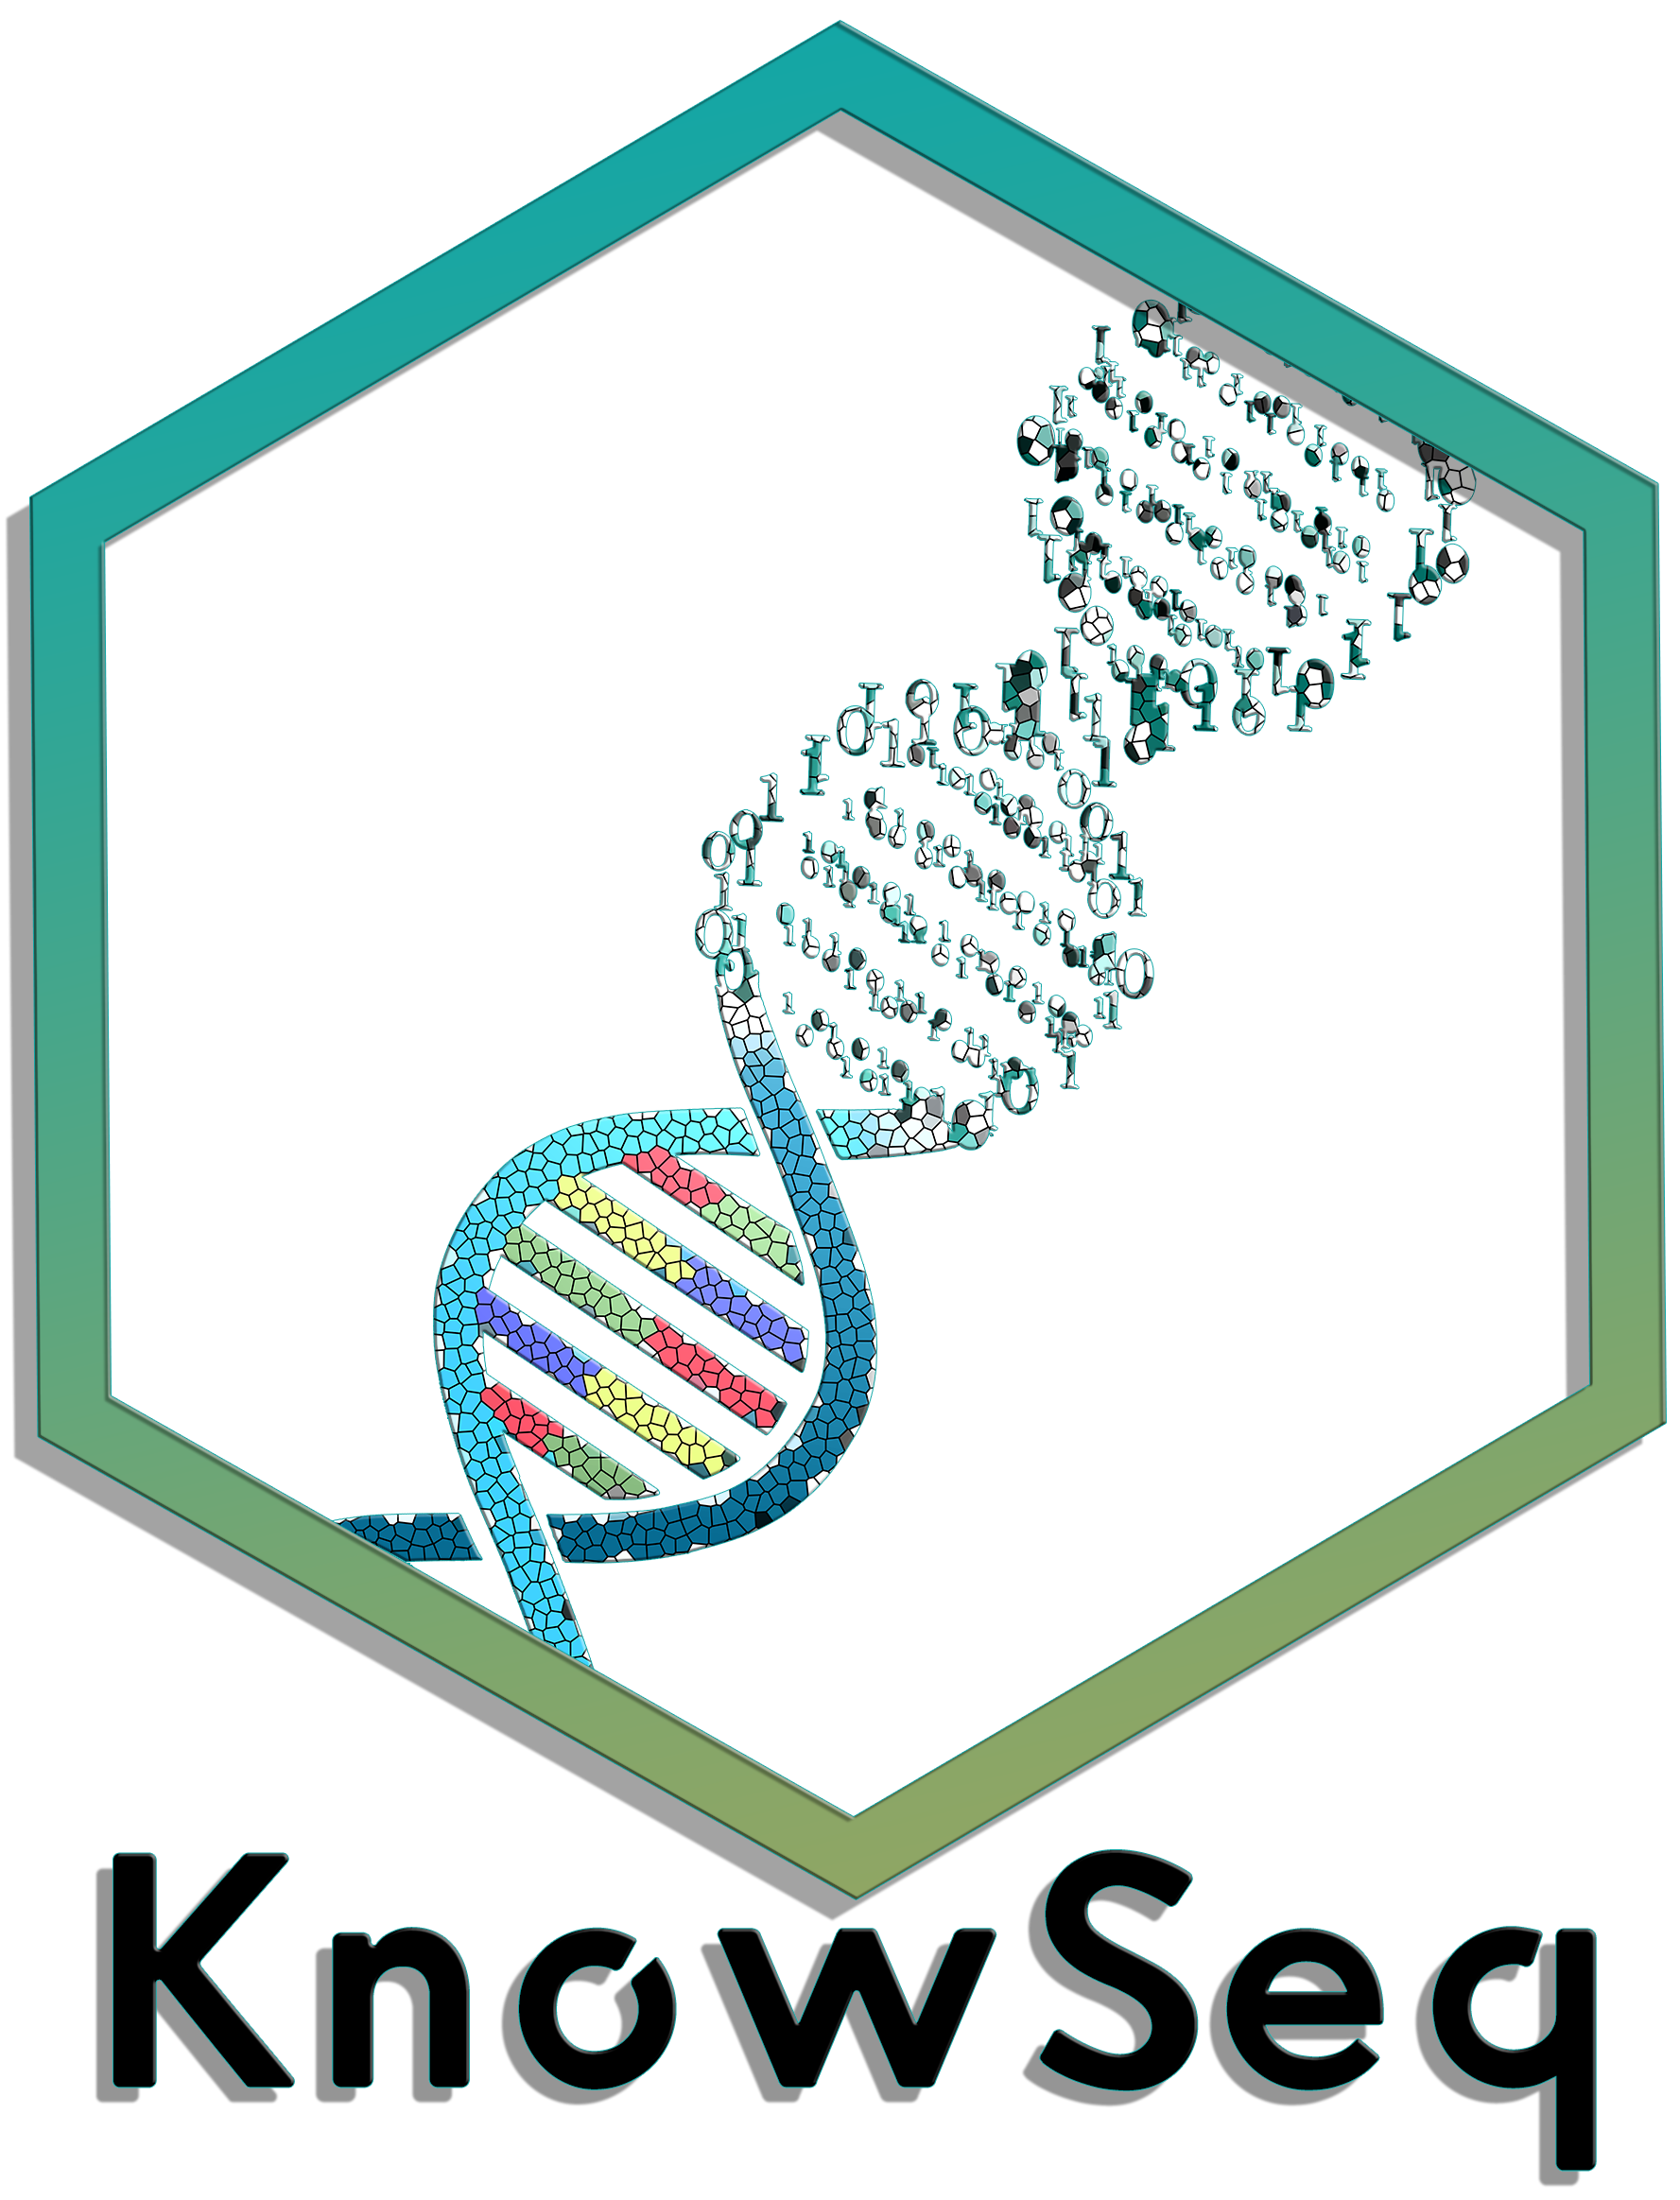
\includegraphics[width=.3\textwidth]{figuras/06_logo_knowseq.png} 
\end{center}

Todo el código de los análisis está disponible en las carpetas \textit{\texttt{analisis\_higado}} y \textit{\texttt{analisis\_cr}} del repositorio de GitHub asociado al trabajo \cite{Redondo-Sanchez2020}. Además, en el fichero \textit{\texttt{session\_info.txt}} se muestran todos los paquetes de \texttt{R} utilizados y sus versiones como resultado de ejecutar \textit{\texttt{devtools::session\_info()}}.\\

Además, para la visualización de datos y resultados del presente trabajo se utilizan técnicas de visualización de datos para una mejor comprensión de los resultados empleando diagramas de Sankey, diagramas de cajas, y mapas de calor.

\subsection{Detección de biomarcadores}

\subsubsection{Preprocesamiento}

Tras descargar los ficheros de GDC Portal y descomprimirlos con \texttt{R} (usando los ficheros \textit{\texttt{analisis\_higado/02\_descompresion}} y \textit{\texttt{analisis\_cr/02\_descompresion}}  en GitHub \cite{Redondo-Sanchez2020}), se preprocesa la información para trabajar con matrices y data.frames.

\subsubsection{Extracción de genes diferencialmente expresados (DEG)}

Se extraen los genes diferencialmente expresados (DEG, por sus siglas en inglés: \textit{Differentially Expressed Genes}) utilizando un p-valor de p = 0,001 y controlando por el efecto batch usando el método SVA (\textit{Surrogate Variable Analysis}) \cite{Leek2012}. El efecto batch es un sesgo que se puede producir al procesar las muestras biológicas por tandas, y puede ocurrir por varias razones como las condiciones del laboratorio, diferencias entre personal, o incluso la hora del día a la que se procesan las muestras \cite{Goh2017, Leek2010}. Para la extracción de DEG se fija además un LFC (\textit{log fold change}) de 1, que se puede entender como que un gen sólo se considera un DEG si una de las dos expresiones de genes (ya sea de tumores o tejidos sanos) es al menos el doble que la otra. Finalmente, los resultados se extraen a una matriz de DEGs.\\

Aunque esta técnica es habitual \cite{Lee2020}, se podría mejorar haciendo la extracción de DEGs mediante validación cruzada para diferentes conjuntos, seleccionando como DEGs aquellos que han sido identificados como tal en todos los folds.

\subsubsection{Partición entrenamiento-test}

Se realiza una partición entrenamiento-test de manera aleatoria con equilibrio de clases: el 75\% de las muestras de cada clase pasan a formar parte del conjunto de entrenamiento y el 25\% restante del conjunto de test.

\subsubsection{Genes más relevantes}

Se utiliza el conjunto de entrenamiento para seleccionar los diez genes más relevantes mediante los tres métodos de selección de características detallados en el capítulo anterior: mRMR, RF y DA.

\subsection{Validación cruzada en entrenamiento}

Se realiza validación cruzada 5-fold para tres algoritmos de clasificación: SVM, RF y kNN. Los parámetros de los clasificadores se optimizan usando los 10 genes más relevantes de cada método de selección de características (mRMR, RF y DA). Para SVM con kernel radial se realiza optimización de los dos parámetros utilizando una rejilla con los valores especificados en la Tabla 13.\\

\textbf{Tabla 13}. Valores de los parámetros que se utilizan para la búsqueda en rejilla de los parámetros óptimos del algoritmo SVM.

\begin{table}[H]
	\centering
	\begin{tabular}{crrrrrrrrr}
		\hline
		\multirow{2}{*}{\textbf{Coste}} & 0    & 0,01 & 0,02         & 0,025                             & 0,03 & 0,04 & 0,05 & 0,06 \\
		& 0,07 & 0,08 & 0,09         & 0,1                               & 0,25 & 0,5  & 0,75 & 0,9  \\ \hline
		\multirow{2}{*}{\textbf{Gamma}} & 0,01 & 0,05 & 0,1 & 0,25 & 0,5  &      &      &      \\
		& 0,75 & 1    & 1,5          & 2                                 & 5    &      &      &      \\ \hline
	\end{tabular}
\end{table}

Posteriormente, para cada algoritmo se usan como variables los $k$ genes más relevantes encontrados cada uno de los tres métodos de selección de características con $k = 1, 2, \hdots, 10$. Por tanto, para cada algoritmo de clasificación (SVM, RF, kNN) se crean 30 modelos distintos. Como el problema a resolver tiene un gran desequilibrio de clases, la medida de evaluación de los modelos escogida es el F1-Score medio de los 5 folds. El mejor modelo (aquel con mayor F1-Score) es posteriormente validado en el conjunto de test.

\subsection{Validación en test}

El mejor modelo encontrado en la fase previa para cada clasificador (SVM, RF, kNN) se utiliza para predecir el tipo de muestra del conjunto de test. Se comparan los resultados predichos con los reales, mostrando las matrices de confusión y los indicadores de evaluación F1-Score y precisión.

\section{Resultados de clasificación biclase para cáncer de hígado}

El código completo del análisis está disponible en el fichero \textit{\texttt{analisis\_higado/\linebreak03\_analisis\_biclase.R}} del repositorio de GitHub asociado al trabajo \cite{Redondo-Sanchez2020}.

\subsection{Detección de biomarcadores}

Para la clasificación biclase en cáncer de hígado se cuenta con 404 tumores y 58 muestras de tejido sano (Tabla 14).\\

\textbf{Tabla 14}. Distribución de tipos de muestra para el análisis de cáncer de hígado biclase.

\begin{table}[H]
	\centering
	\begin{tabular}{lcc}
		\cline{2-3}
		& \textbf{Número de casos} & \textbf{Porcentaje} \\ \hline
		\textbf{Tumores}     & 404        & 87,4\%              \\
		\textbf{Tejido sano} & 58         & 12,6\%              \\ \hline
		\textbf{Total}       & 462        & 100\%               \\ \hline
	\end{tabular}
\end{table}

De los 24.645 genes presentes en los datos se extraen 2.274 genes que presentan en su expresión diferencias significativas entre las muestras de tumores y las de tejido sano. En la Tabla 15 se muestra la partición entrenamiento - test realizada y en la Figura 7 se representa en un diagrama de Sankey.\\

\newpage
\textbf{Tabla 15}. Distribución entrenamiento-test según tipo de muestra y proporción entre clases (tumores/tejido sano) para el análisis de hígado biclase.\\

\begin{table}[H]
	\centering
	\begin{tabular}{lccc}
		\cline{2-4}
		\multicolumn{1}{c}{\textbf{}}     & \textbf{Total} & \textbf{Entrenamiento} & \textbf{Test} \\ \hline
		\textbf{Tumores}                  & 404 (100\%)    & 303 (75,0\%)             & 101 (25,0\%)    \\
		\textbf{Tejido sano}                    & 58 (100\%)     & 44 (75,9\%)            & 14 (24,1\%)   \\ \hline
		\textbf{\begin{tabular}[c]{@{}l@{}}Proporción\\ tumores/sanos\end{tabular}} & 6,97           & 6,89                   & 7,21          \\ \hline
	\end{tabular}
\end{table}

\begin{center}
	\textbf{Figura 7}. Diagrama de Sankey mostrando la partición entrenamiento-test realizada según tipo de muestra para el análisis de hígado biclase.
\end{center}
\begin{center}
	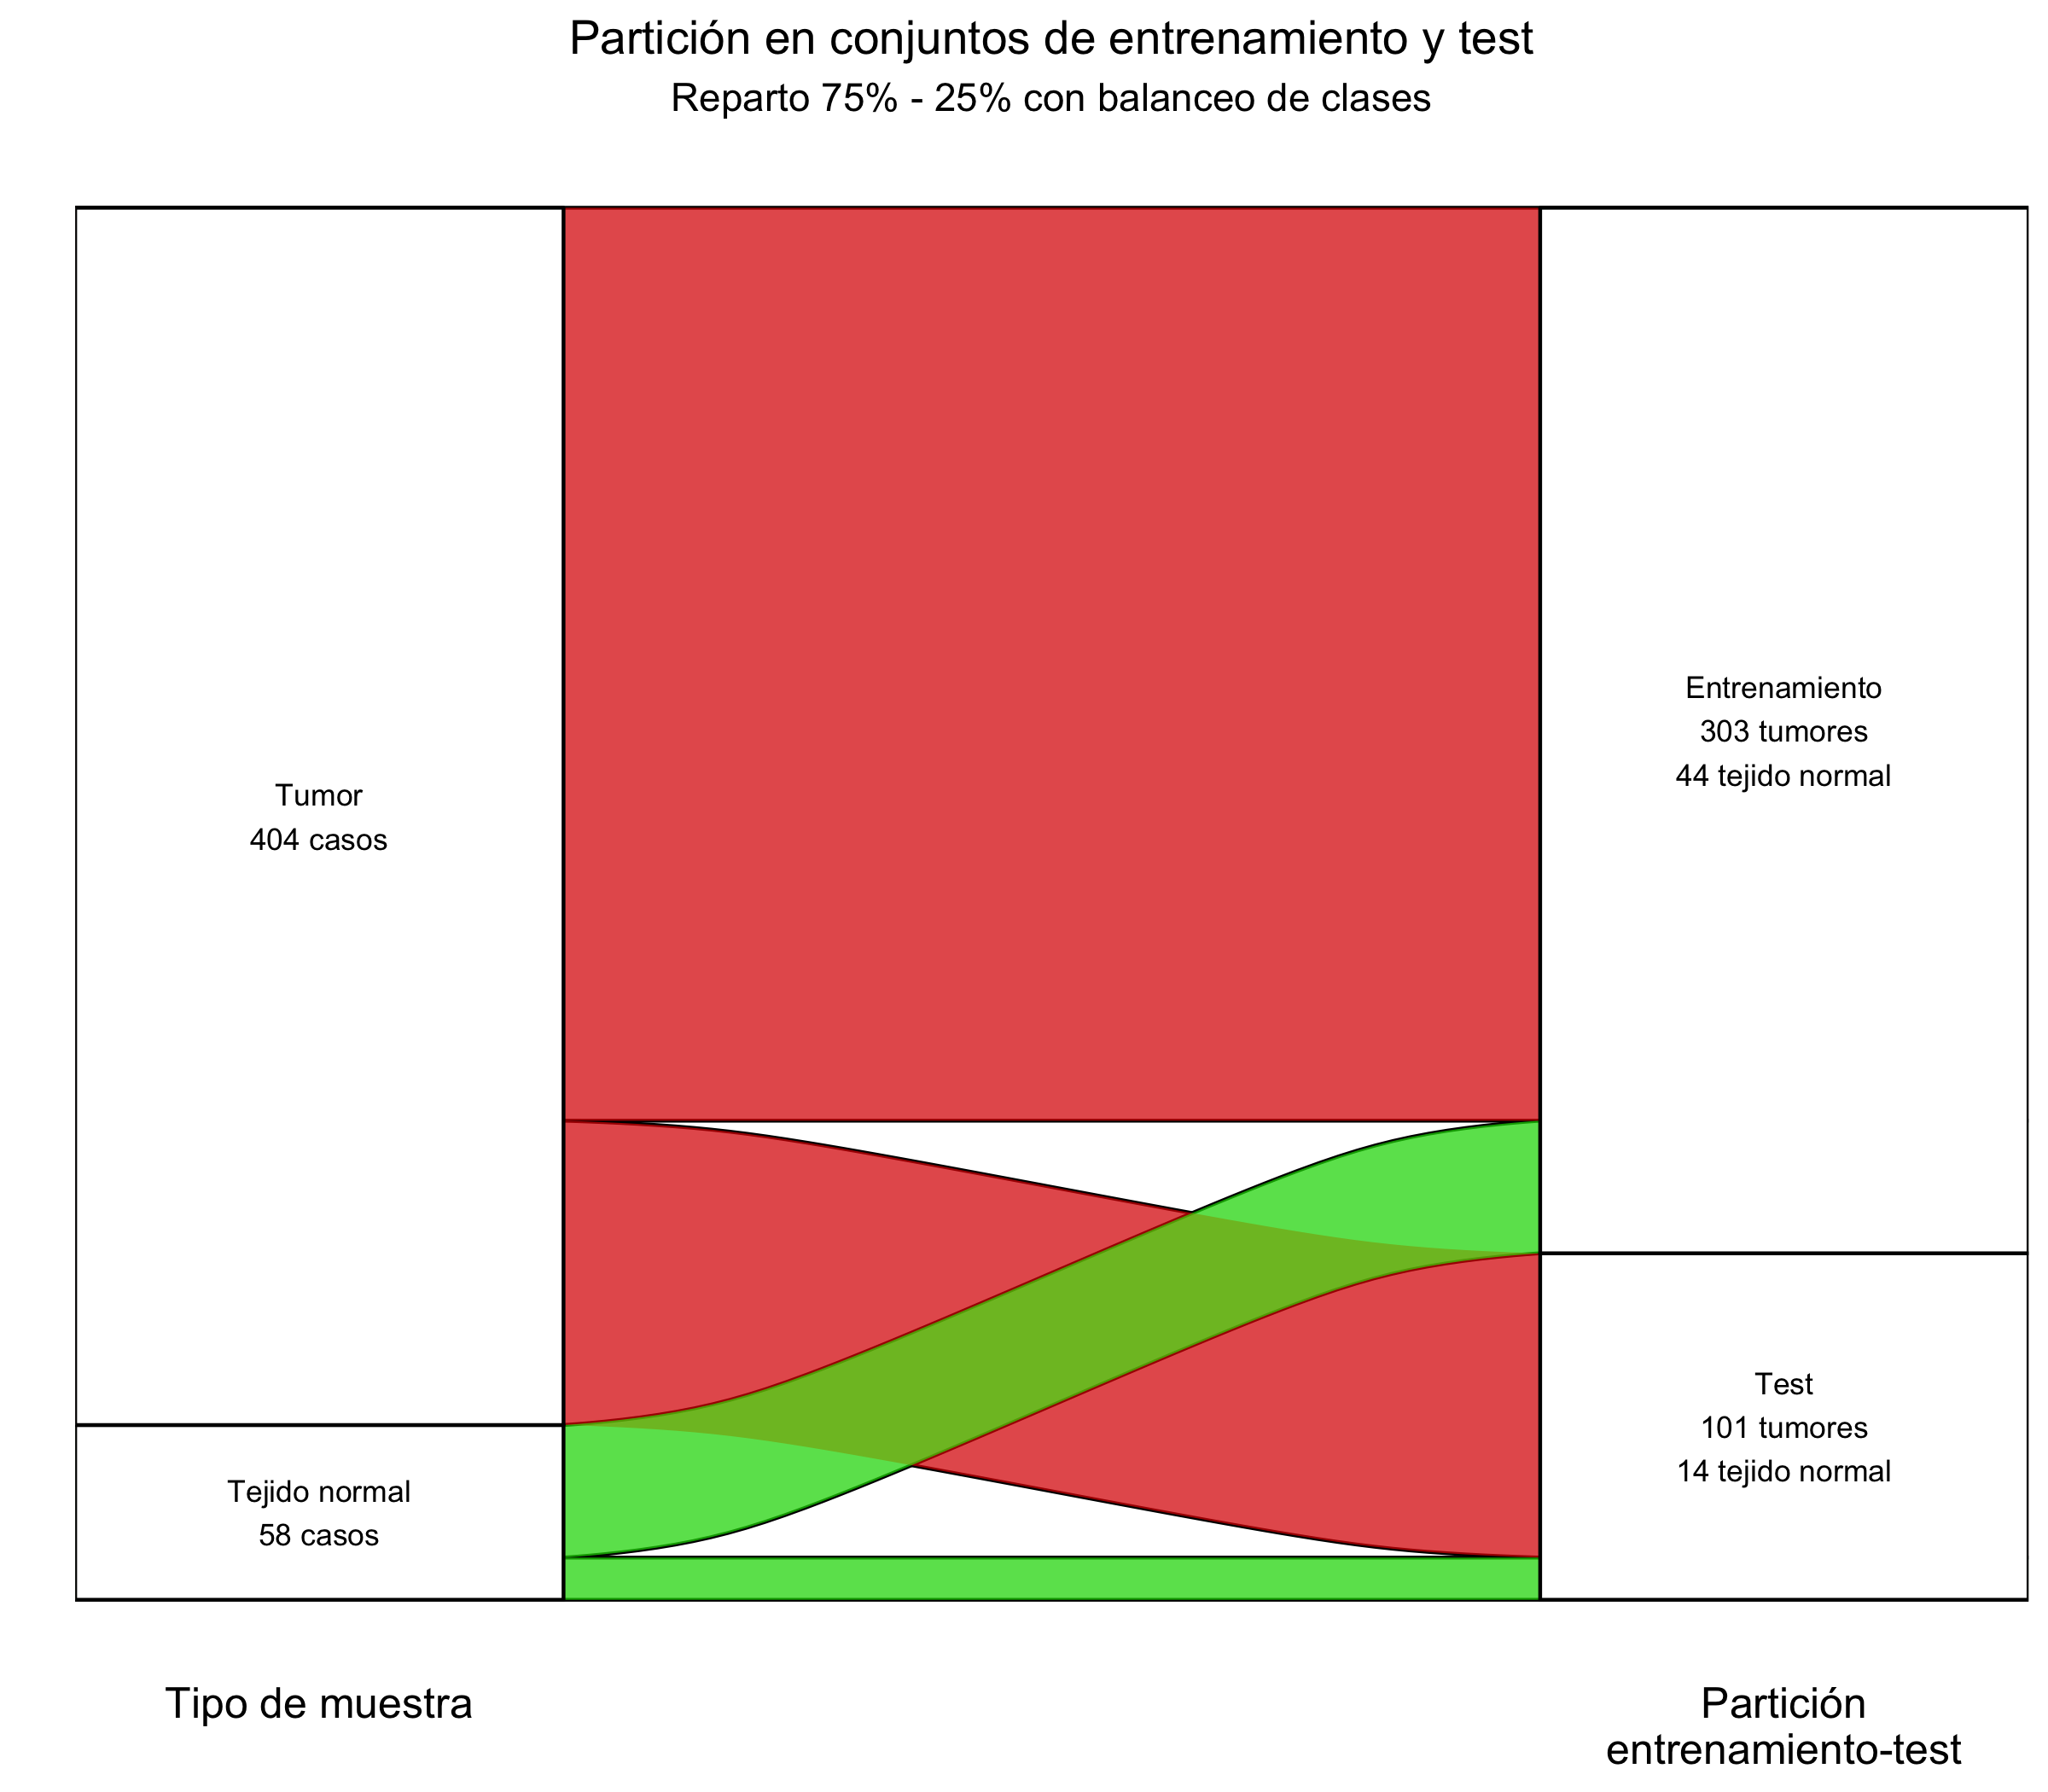
\includegraphics[width=.75\textwidth]{figuras/07_higado_biclase_sankey.png}
\end{center}

A continuación se muestran los diez genes más relevantes encontrados por cada método de selección de características:\\

\newpage
\textbf{Tabla 16}. Diez genes más relevantes según los distintos métodos de selección de características para el análisis de hígado biclase.

\begin{table}[H]
	\centering
	\begin{tabular}{cccc}
		\hline
		\textbf{Ranking} & \textbf{mRMR} & \textbf{RF} & \textbf{DA} \\ \hline
		1                & ANGPTL6       & ANGPTL6     & TERT        \\
		2                & THY1          & PTH1R       & RSPO3       \\
		3                & ADAMTS13      & ADAMTS13    & HOXA13      \\
		4                & CELSR3        & BMPER       & SIX1        \\
		5                & CCNE1         & PRC1        & TOP2A       \\
		6                & CDH13         & CLEC4G      & GPC3        \\
		7                & C14orf180     & VIPR1       & SSX1        \\
		8                & GABRD         & CLEC4M      & BUB1B       \\
		9                & AP000439.2    & OIT3        & RET         \\
		10               & CEP152        & GABRD       & ESR1        \\ \hline
	\end{tabular}
\end{table}

Se observa que tres genes han sido valorados como relevantes para los algoritmos de mRMR y RF:  ANGPTL6, ADAMTS13 y GABRD.

\subsection{Validación cruzada en entrenamiento - SVM}

En la Tabla 17 se muestran los parámetros óptimos de SVM obtenidos tras la búsqueda en rejilla.\\

\textbf{Tabla 17}. Parámetros óptimos de SVM encontrados para los 10 genes más relevantes de cada método de selección de características.

\begin{table}[H]
	\centering
	\begin{tabular}{cccc}
		\hline
		\textbf{Parámetro} & \textbf{mRMR} & \textbf{RF} & \textbf{DA} \\ \hline
		Coste                &    0,05 &    0,75     &   0,1       \\
		Gamma               &     0,05    &     0,1   & 0,06        \\ \hline
	\end{tabular}
\end{table}

Para estos parámetros óptimos, en la Figura 8 se muestran las medidas de evaluación medias obtenidas en las 5 fold.\\

\newpage
\begin{center}
\textbf{Figura 8}. Mapa de calor con valores medios y desviación típica de los 5-fold de F1-Score, precisión, sensibilidad y especificidad de SVM según método de selección de características y número de genes usados.
\end{center}
\begin{center}
	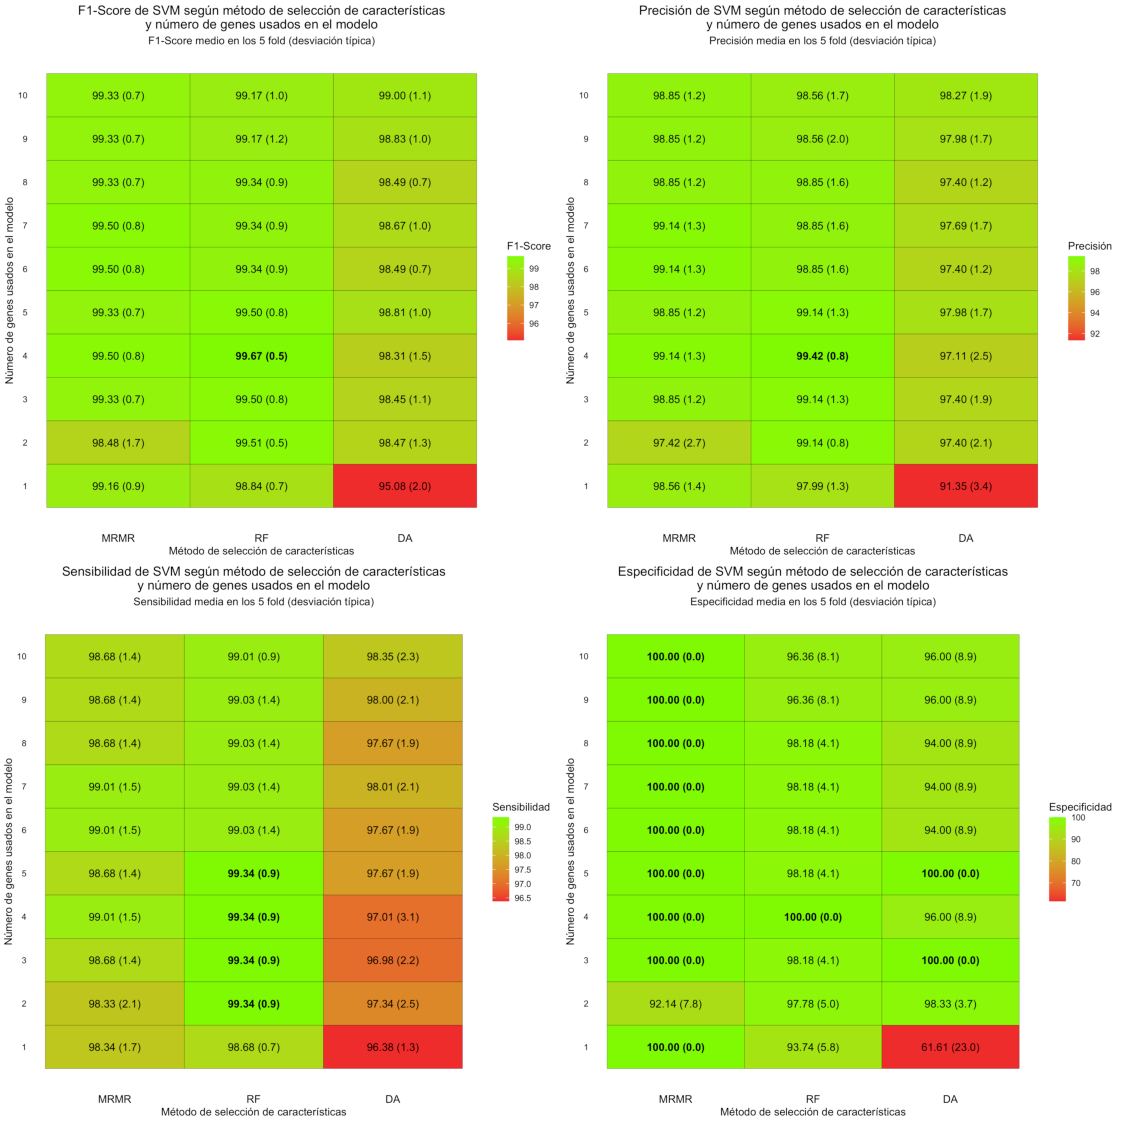
\includegraphics[width=1\textwidth]{figuras/08_higado_biclase_heatmap_svm.pdf} 
\end{center}

El mejor F1-Score para SVM se obtiene con 4 genes seleccionados con RF (99,67\%), configuración que obtiene también los mejores valores de precisión (99,42\%), sensibilidad (99,34\%) y especificidad (100\%). Los 4 genes seleccionados son: ANGPTL6, PTH1R, ADAMTS13 y BMPER. Se analiza la expresión de genes de estos 4 genes, utilizando para ello un mapa de calor (Figura 9) y diagramas de caja (Figura 10).

\newpage
\begin{center}
\textbf{Figura 9}. Mapa de calor de expresión de genes por tipo de muestra (columna izquierda: rojo = tumor, verde = tejido sano) en los 4 genes más relevantes encontrados en el mejor modelo de SVM con RF como método de selección de características.
\end{center}
\begin{center}
	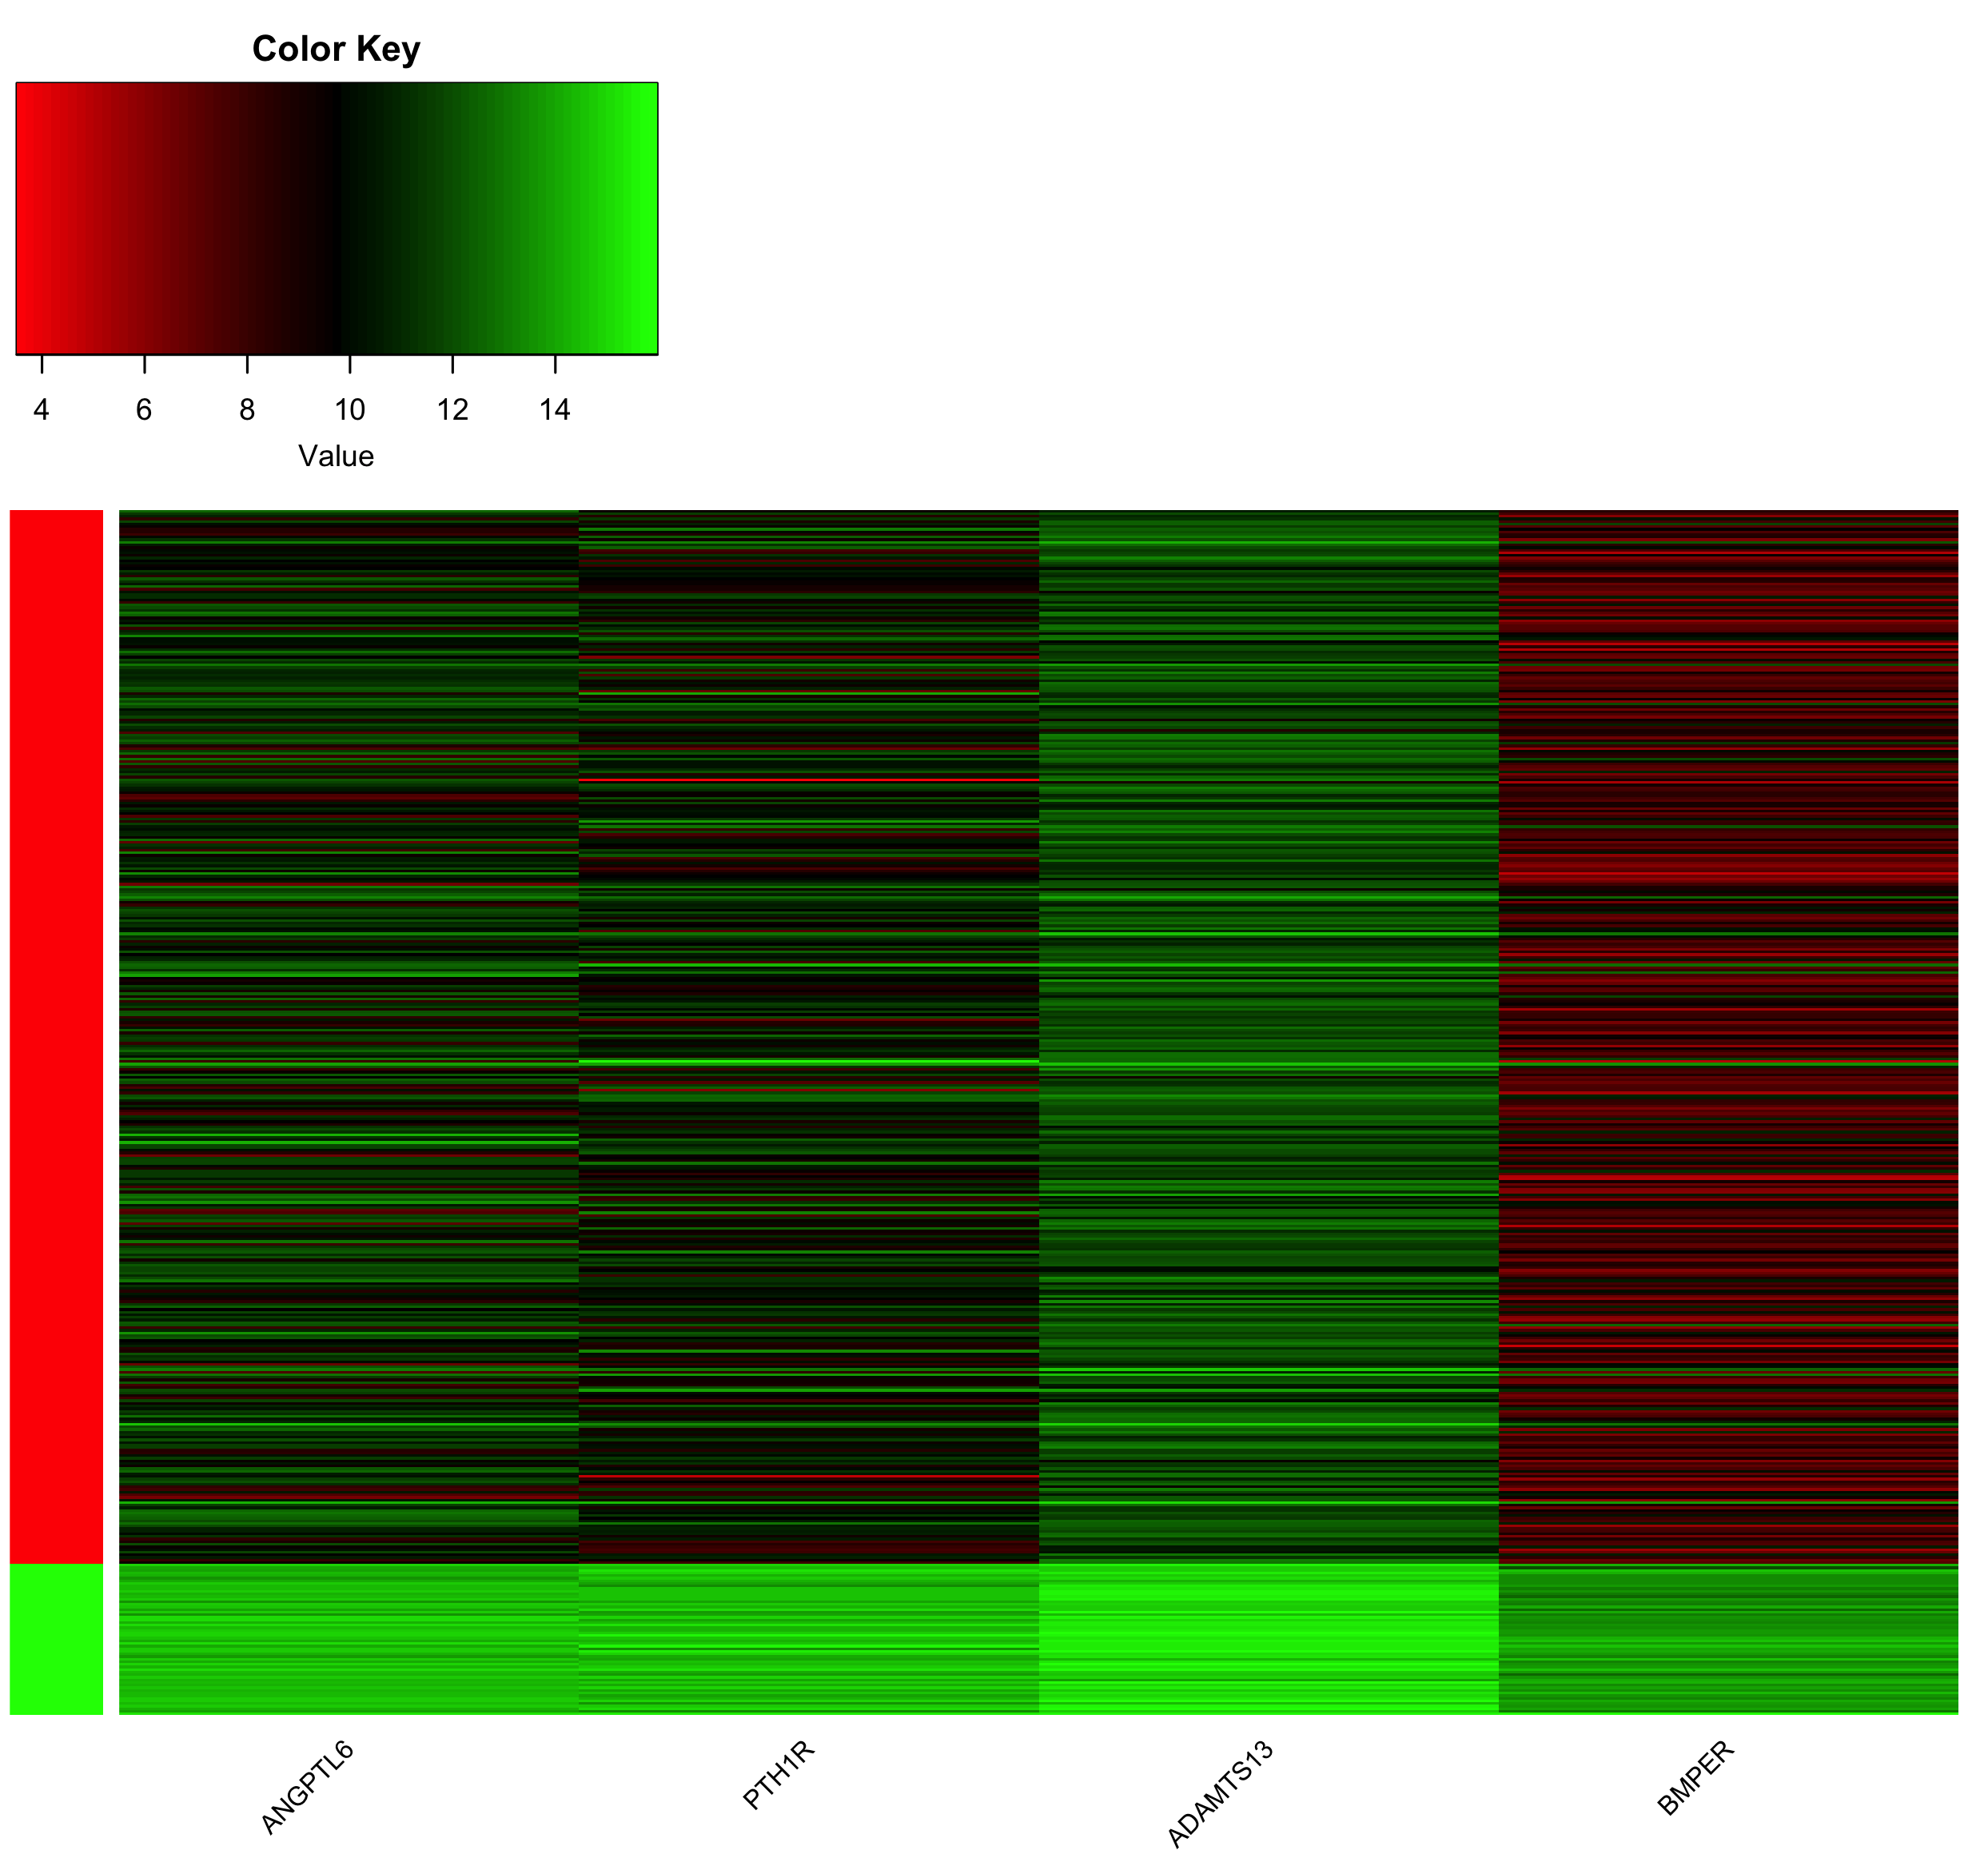
\includegraphics[width=1\textwidth]{figuras/09_higado_biclase_16_svm_heatmap_mejor_metodo.png} 
\end{center}

En el mapa de calor se observa que en general los genes seleccionados están sobreexpresados en tejidos sanos, e inhibidos en tejidos tumorales.

\newpage
\begin{center}
\textbf{Figura 10}. Diagrama de caja de expresión de genes por tipo de muestra en los 4 genes más relevantes encontrados en el mejor modelo de SVM con RF como método de selección de características.
\end{center}
\begin{center}
	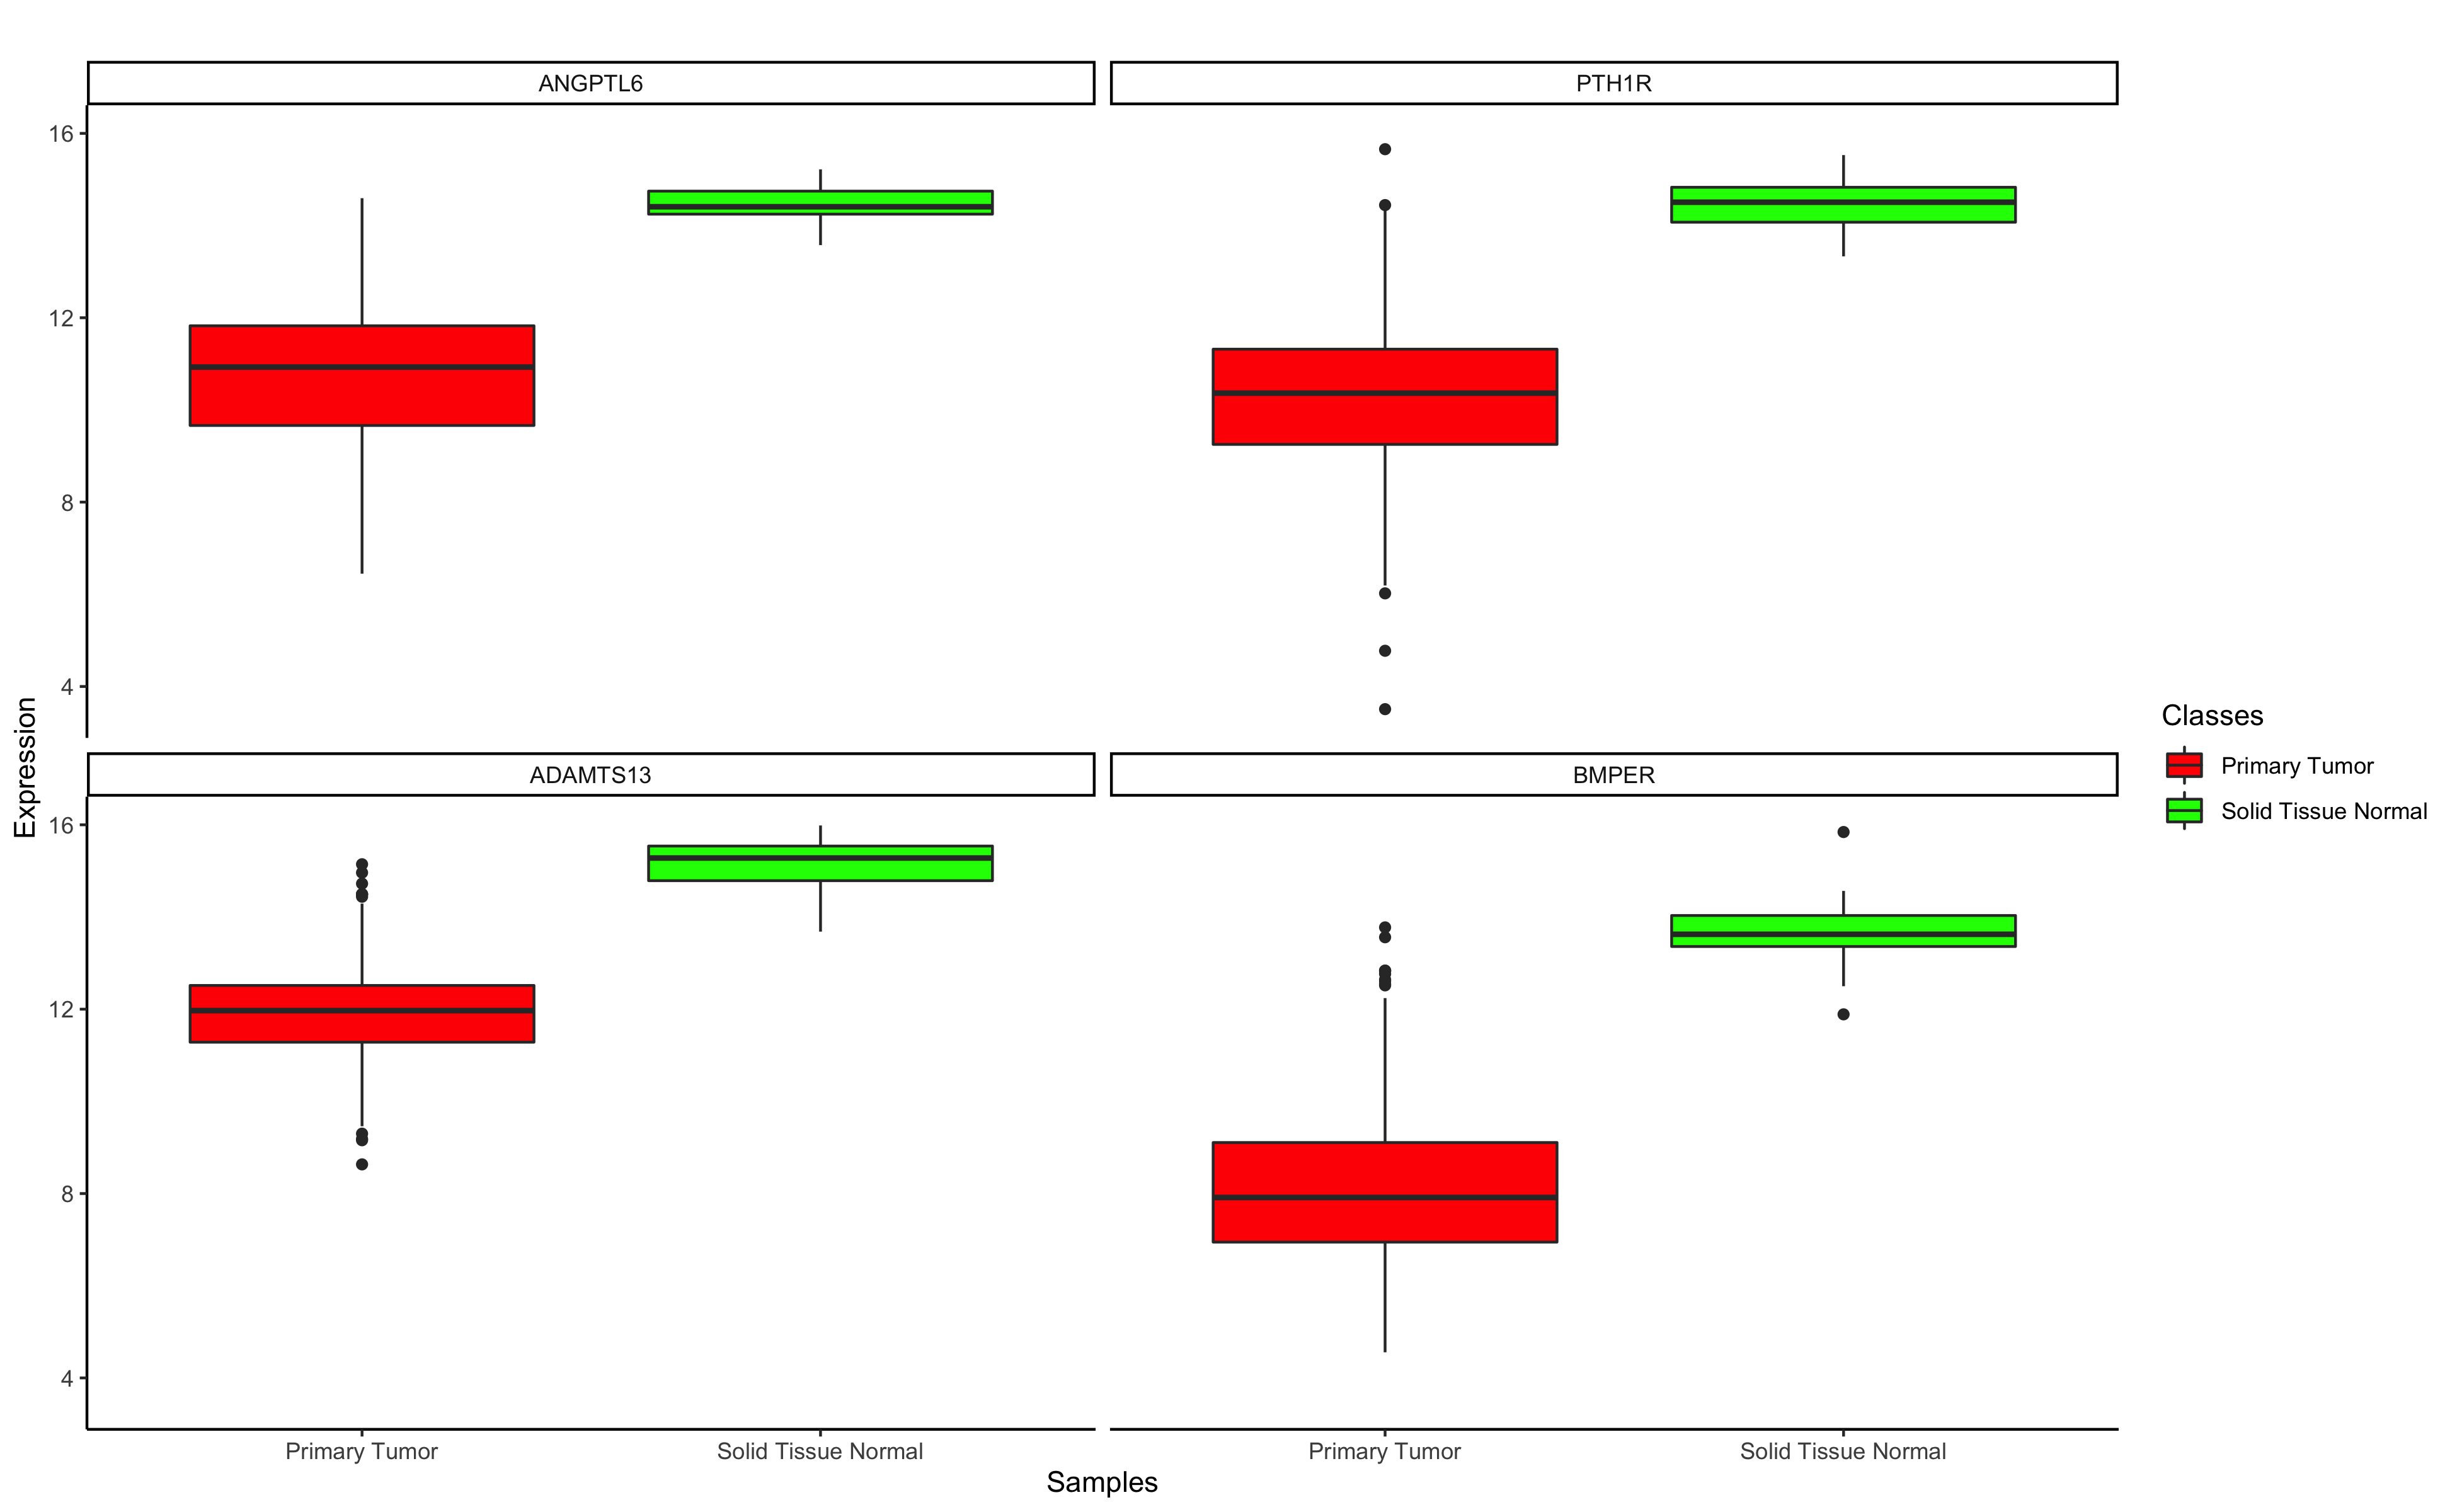
\includegraphics[width=1\textwidth]{figuras/10_higado_biclase_17_svm_boxplots_mejor_metodo.png} 
\end{center}

El diagrama de caja aporta cierta información adicional al mapa de calor, ya que en algunos genes se detectan outliers y se observa mejor el posible solapamiento entre la expresión de genes para tumores y tejidos sanos.

\newpage
\subsection{Validación cruzada en entrenamiento - RF}

En la Figura 11 se muestran las medidas de evaluación medias obtenidas en las 5 fold.\\

\begin{center}
\textbf{Figura 11}. Mapa de calor con valores medios y desviación típica de los 5-fold de F1-Score, precisión, sensibilidad y especificidad de RF según método de selección de características y número de genes usados.
\end{center}
\begin{center}
	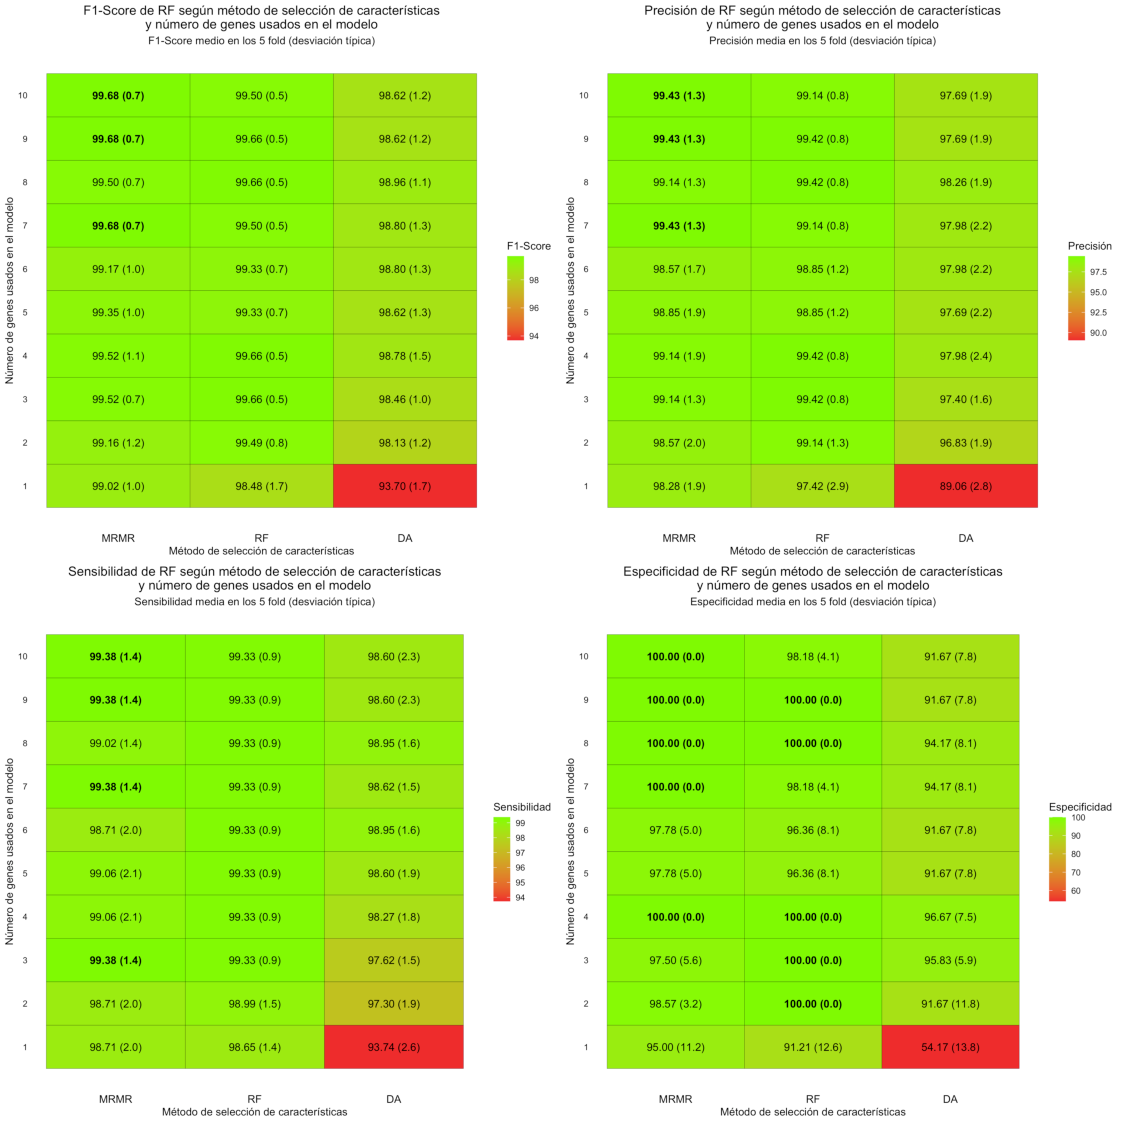
\includegraphics[width=1\textwidth]{figuras/11_higado_biclase_heatmap_rf.pdf} 
\end{center}

Para random forest el mejor F1-Score (99,68\%) se obtiene con el método mRMR considerando 7, 9 o 10 genes. Se selecciona aquel método que tiene menor número de genes: mRMR con 7 genes. Los 7 genes seleccionados son: ANGPTL6, THY1, ADAMTS13, CELSR3, CCNE1, CDH13 y C14orf180. Se analiza su expresión por tipo de muestra, utilizando para ello un mapa de calor (Figura 12) y diagramas de caja (Figura 13).\\

\begin{center}
\textbf{Figura 12}. Mapa de calor de expresión de genes por tipo de muestra (columna izquierda: rojo = tumor, verde = tejido sano) en los 4 genes más relevantes encontrados en el mejor modelo de RF con RF como método de selección de características.
\end{center}
\begin{center}
	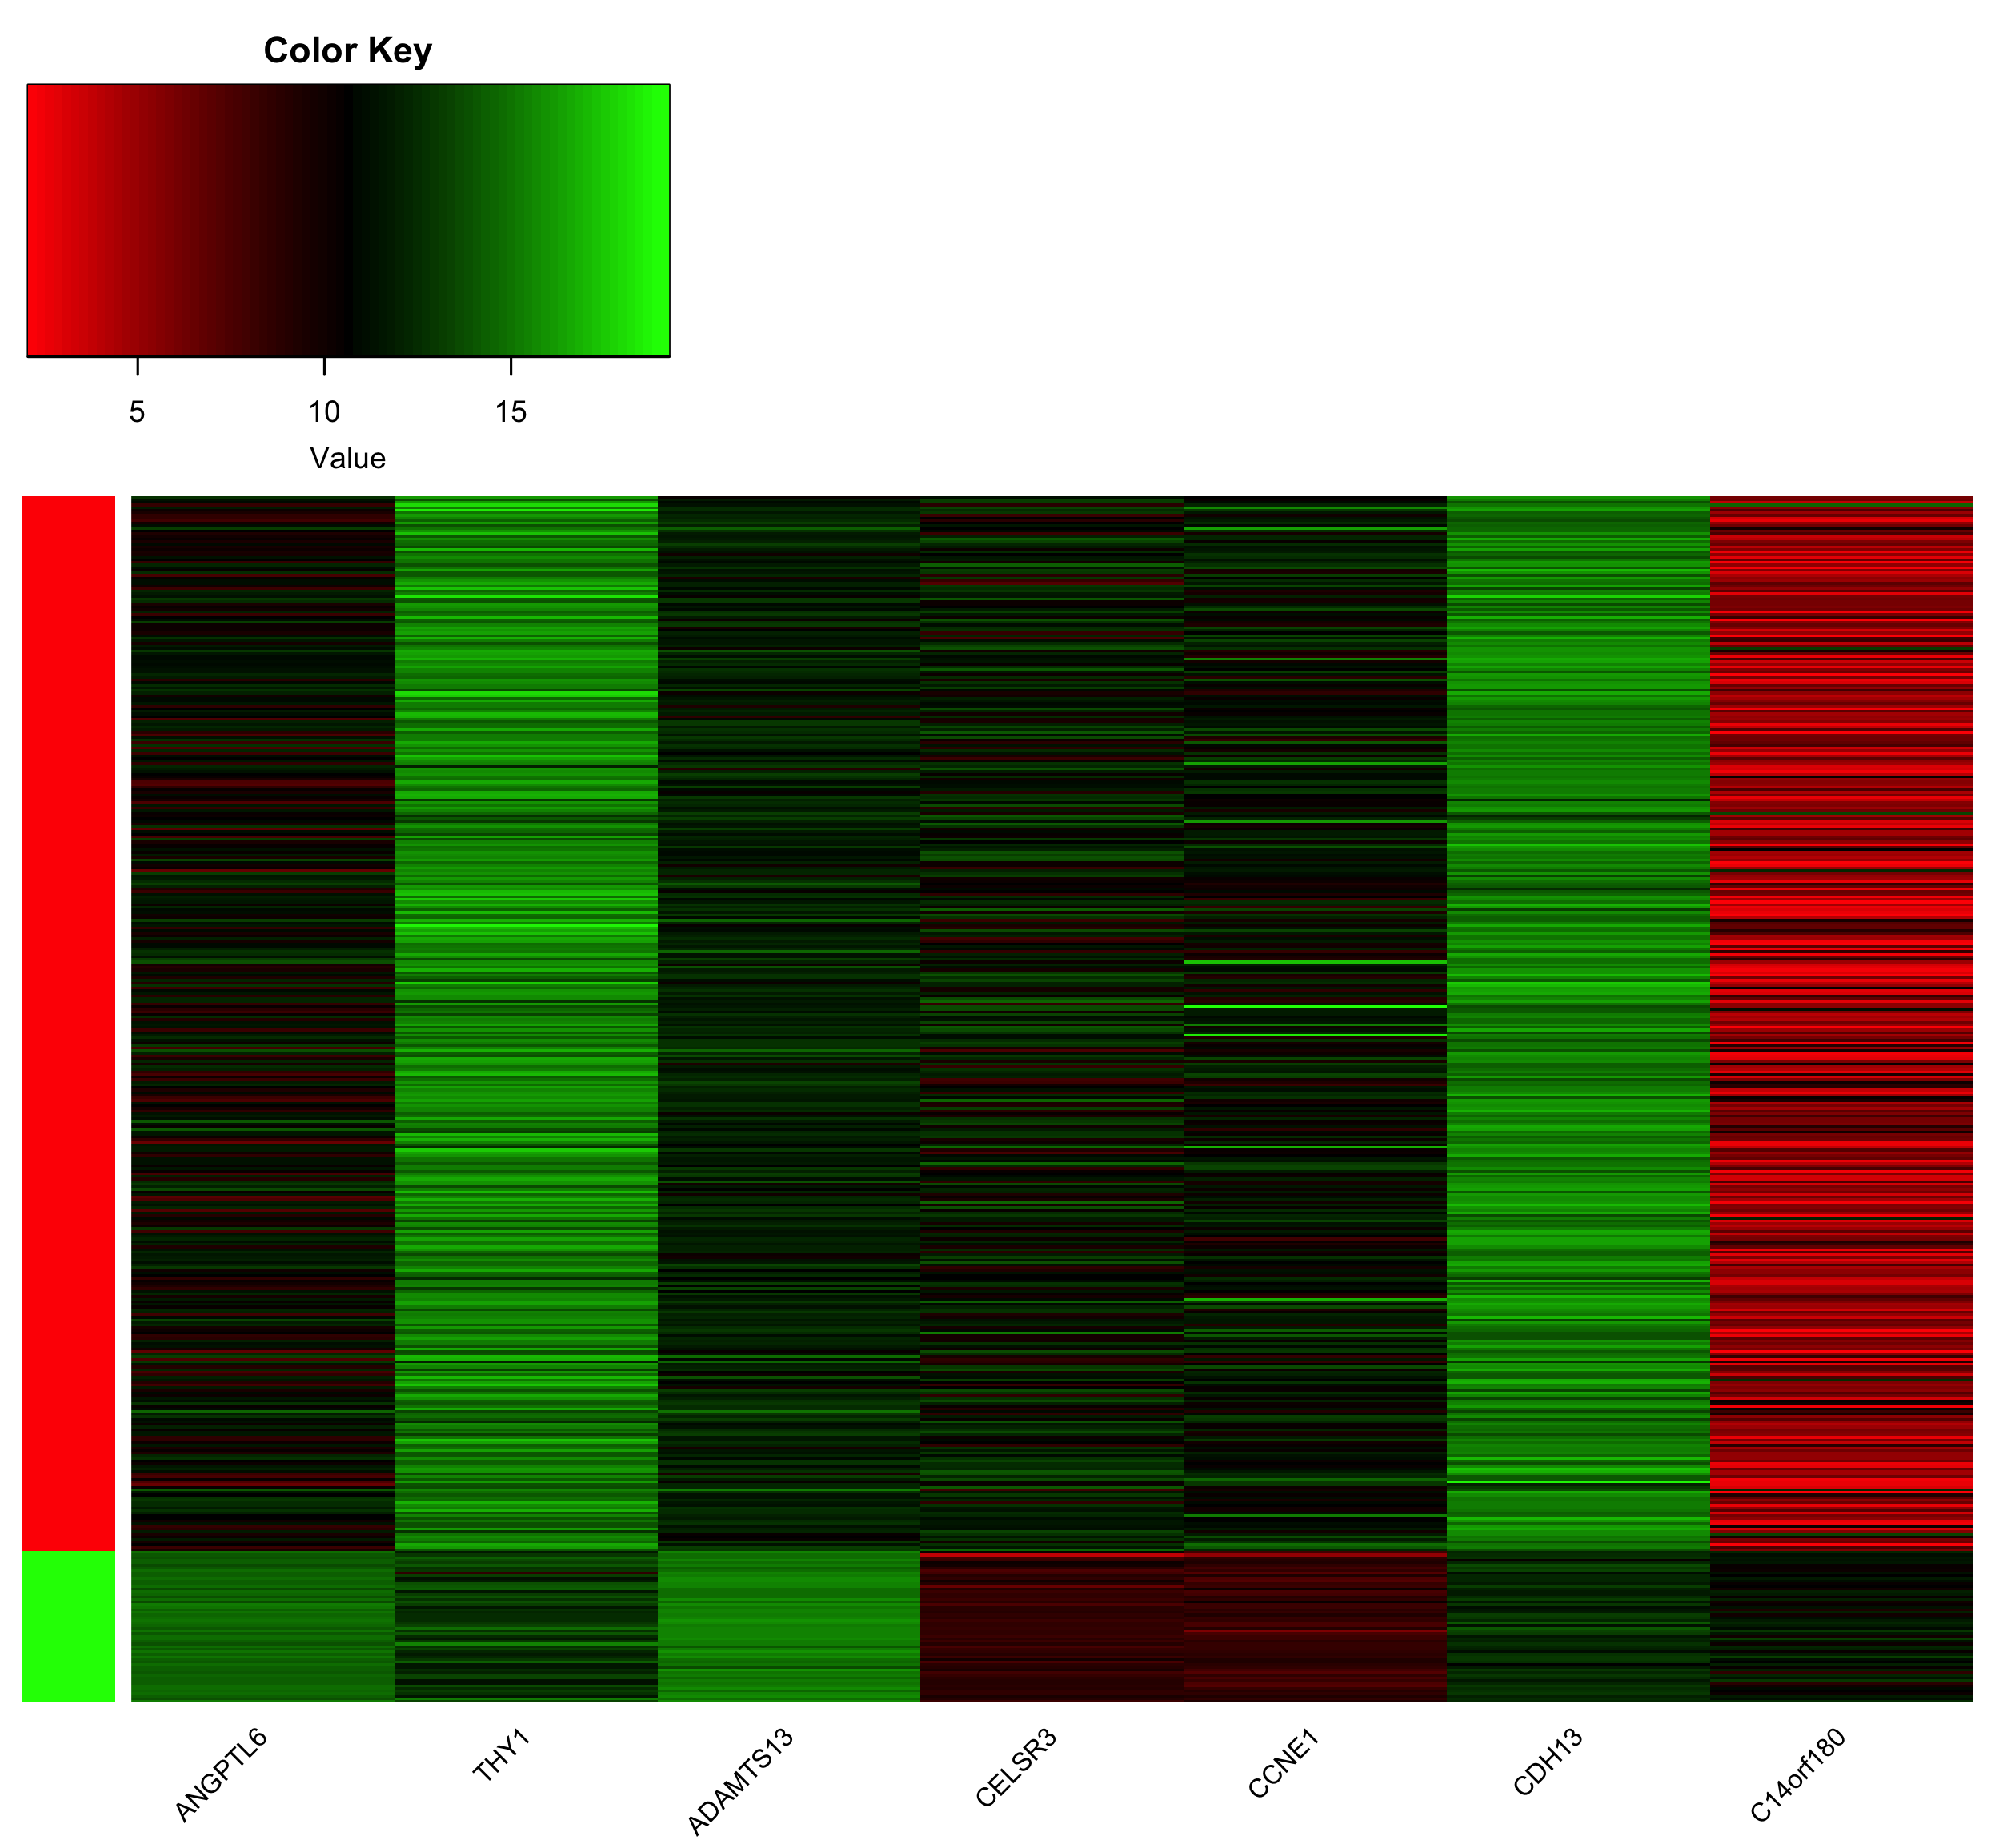
\includegraphics[width=1\textwidth]{figuras/12_higado_biclase_29_rf_heatmap_mejor_metodo.png} 
\end{center}

\newpage
\begin{center}
	\textbf{Figura 13}. Diagrama de caja de expresión de genes por tipo de muestra en los 4 genes más relevantes encontrados en el mejor modelo de RF con RF como método de selección de características.
\end{center}
\begin{center}
	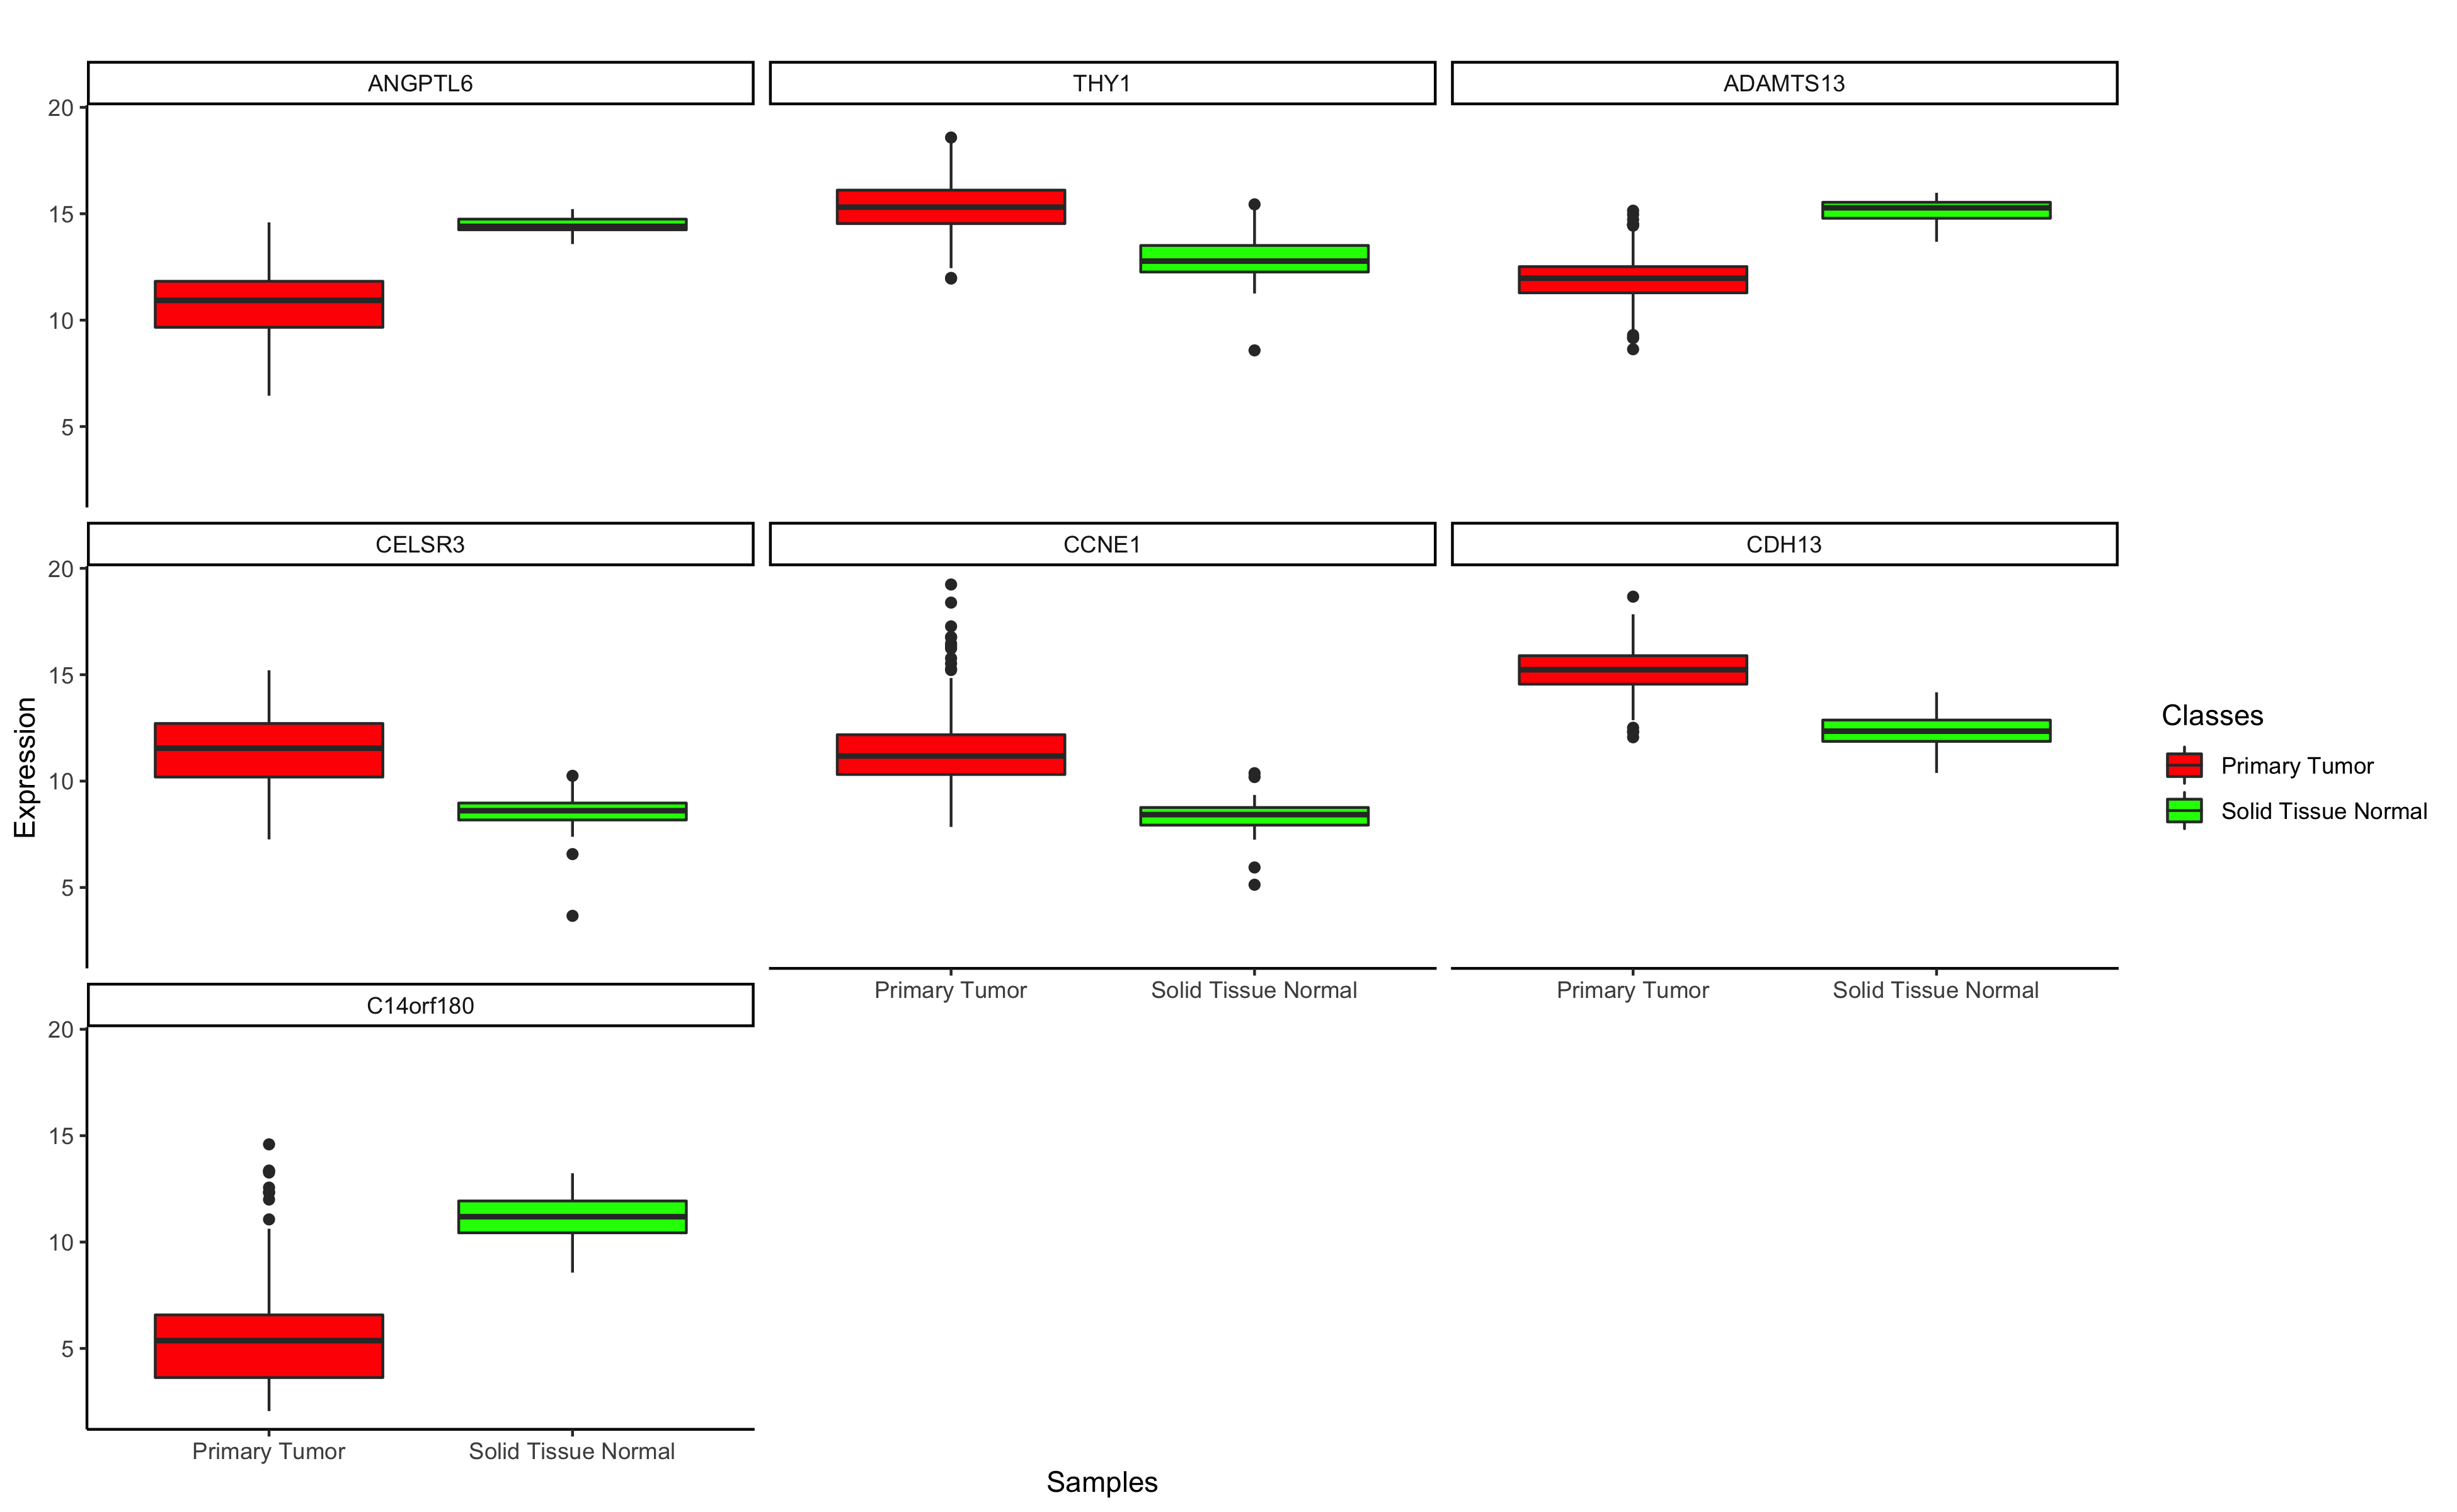
\includegraphics[width=1\textwidth]{figuras/13_higado_biclase_30_rf_boxplots_mejor_metodo.png} 
\end{center}

\subsection{Validación cruzada en entrenamiento - kNN}

El número óptimo de vecinos para los 10 genes más relevantes es 7 para mRMR y DA y 5 para RF (Tabla 18).\\

\textbf{Tabla 18}. Número óptimo de vecinos encontrado para los 10 genes más relevantes de cada método de selección de características.

\begin{table}[H]
	\centering
	\begin{tabular}{cccc}
		\cline{2-4}
		\textbf{} & \textbf{mRMR} & \textbf{RF} & \textbf{DA} \\ \hline
		k                &    7 &    5     &   7      \\ \hline
	\end{tabular}
\end{table}

En la Figura 14 se muestran las medidas de evaluación medias obtenidas en las 5 fold.\\

\newpage
\begin{center}
\textbf{Figura 14}. Mapa de calor con valores medios y desviación típica de los 5-fold de F1-Score, precisión, sensibilidad y especificidad de kNN según método de selección de características y número de genes usados.
\end{center}
\begin{center}
	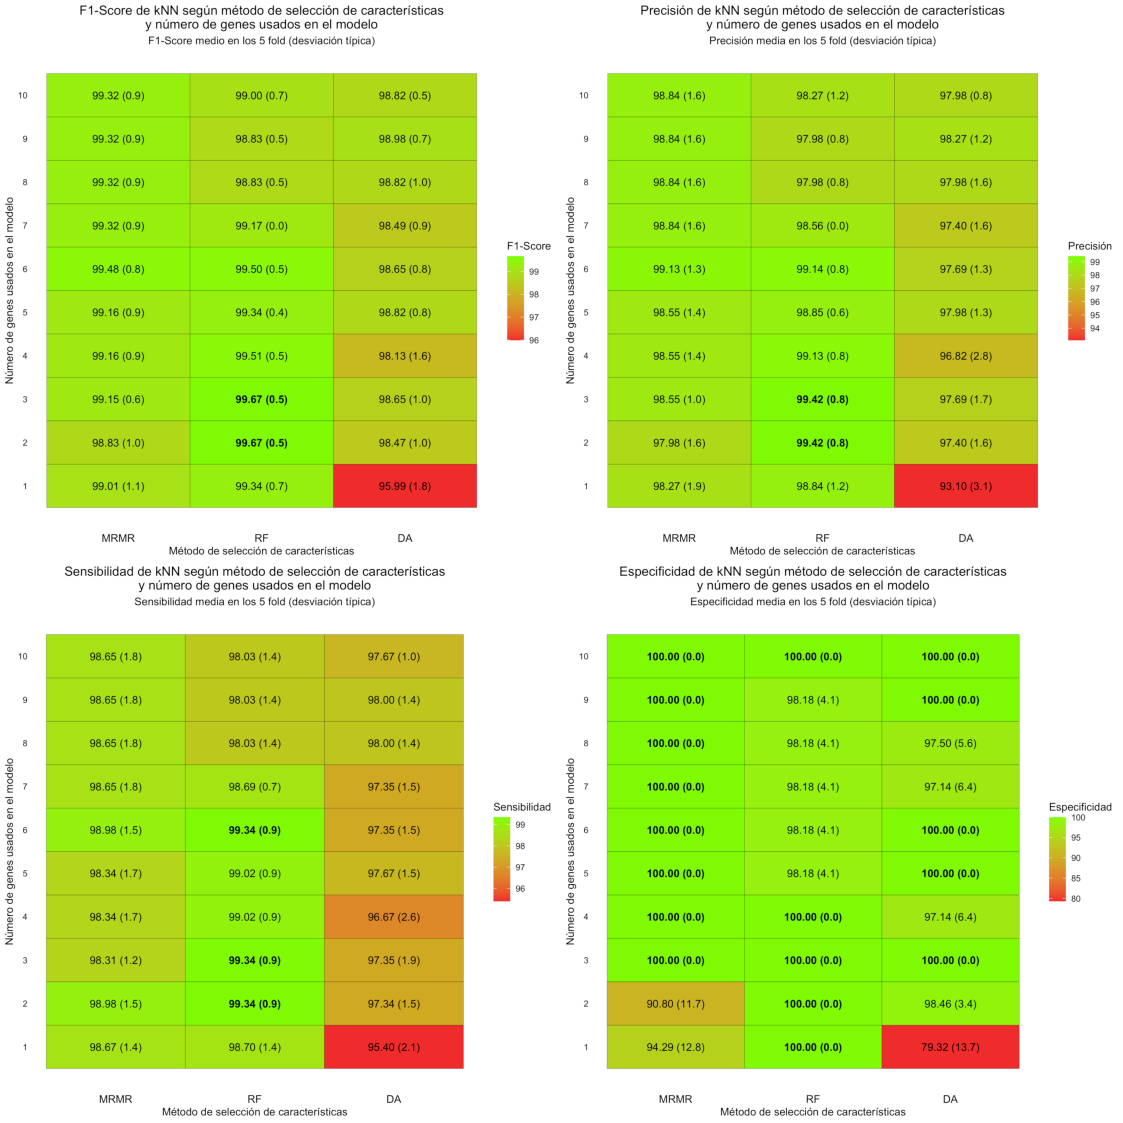
\includegraphics[width=1\textwidth]{figuras/14_higado_biclase_heatmap_knn.pdf} 
\end{center}

Para kNN, el mejor F1-Score (99,68\%) se obtiene con el método RF para 2 y 3 genes. Se selecciona aquel método que tiene menor número de genes: RF con 2 genes. Los 2 genes seleccionados son: ANGPTL6 y PTH1R. Se analiza su expresión de genes, utilizando para ello un mapa de calor (Figura 15) y diagramas de caja (Figura 16).

\newpage
\begin{center}
\textbf{Figura 15}. Mapa de calor de expresión de genes por tipo de muestra (columna izquierda: rojo = tumor, verde = tejido sano) en los 2 genes más relevantes encontrados en el mejor modelo de kNN con RF como método de selección de características.
\end{center}
\begin{center}
	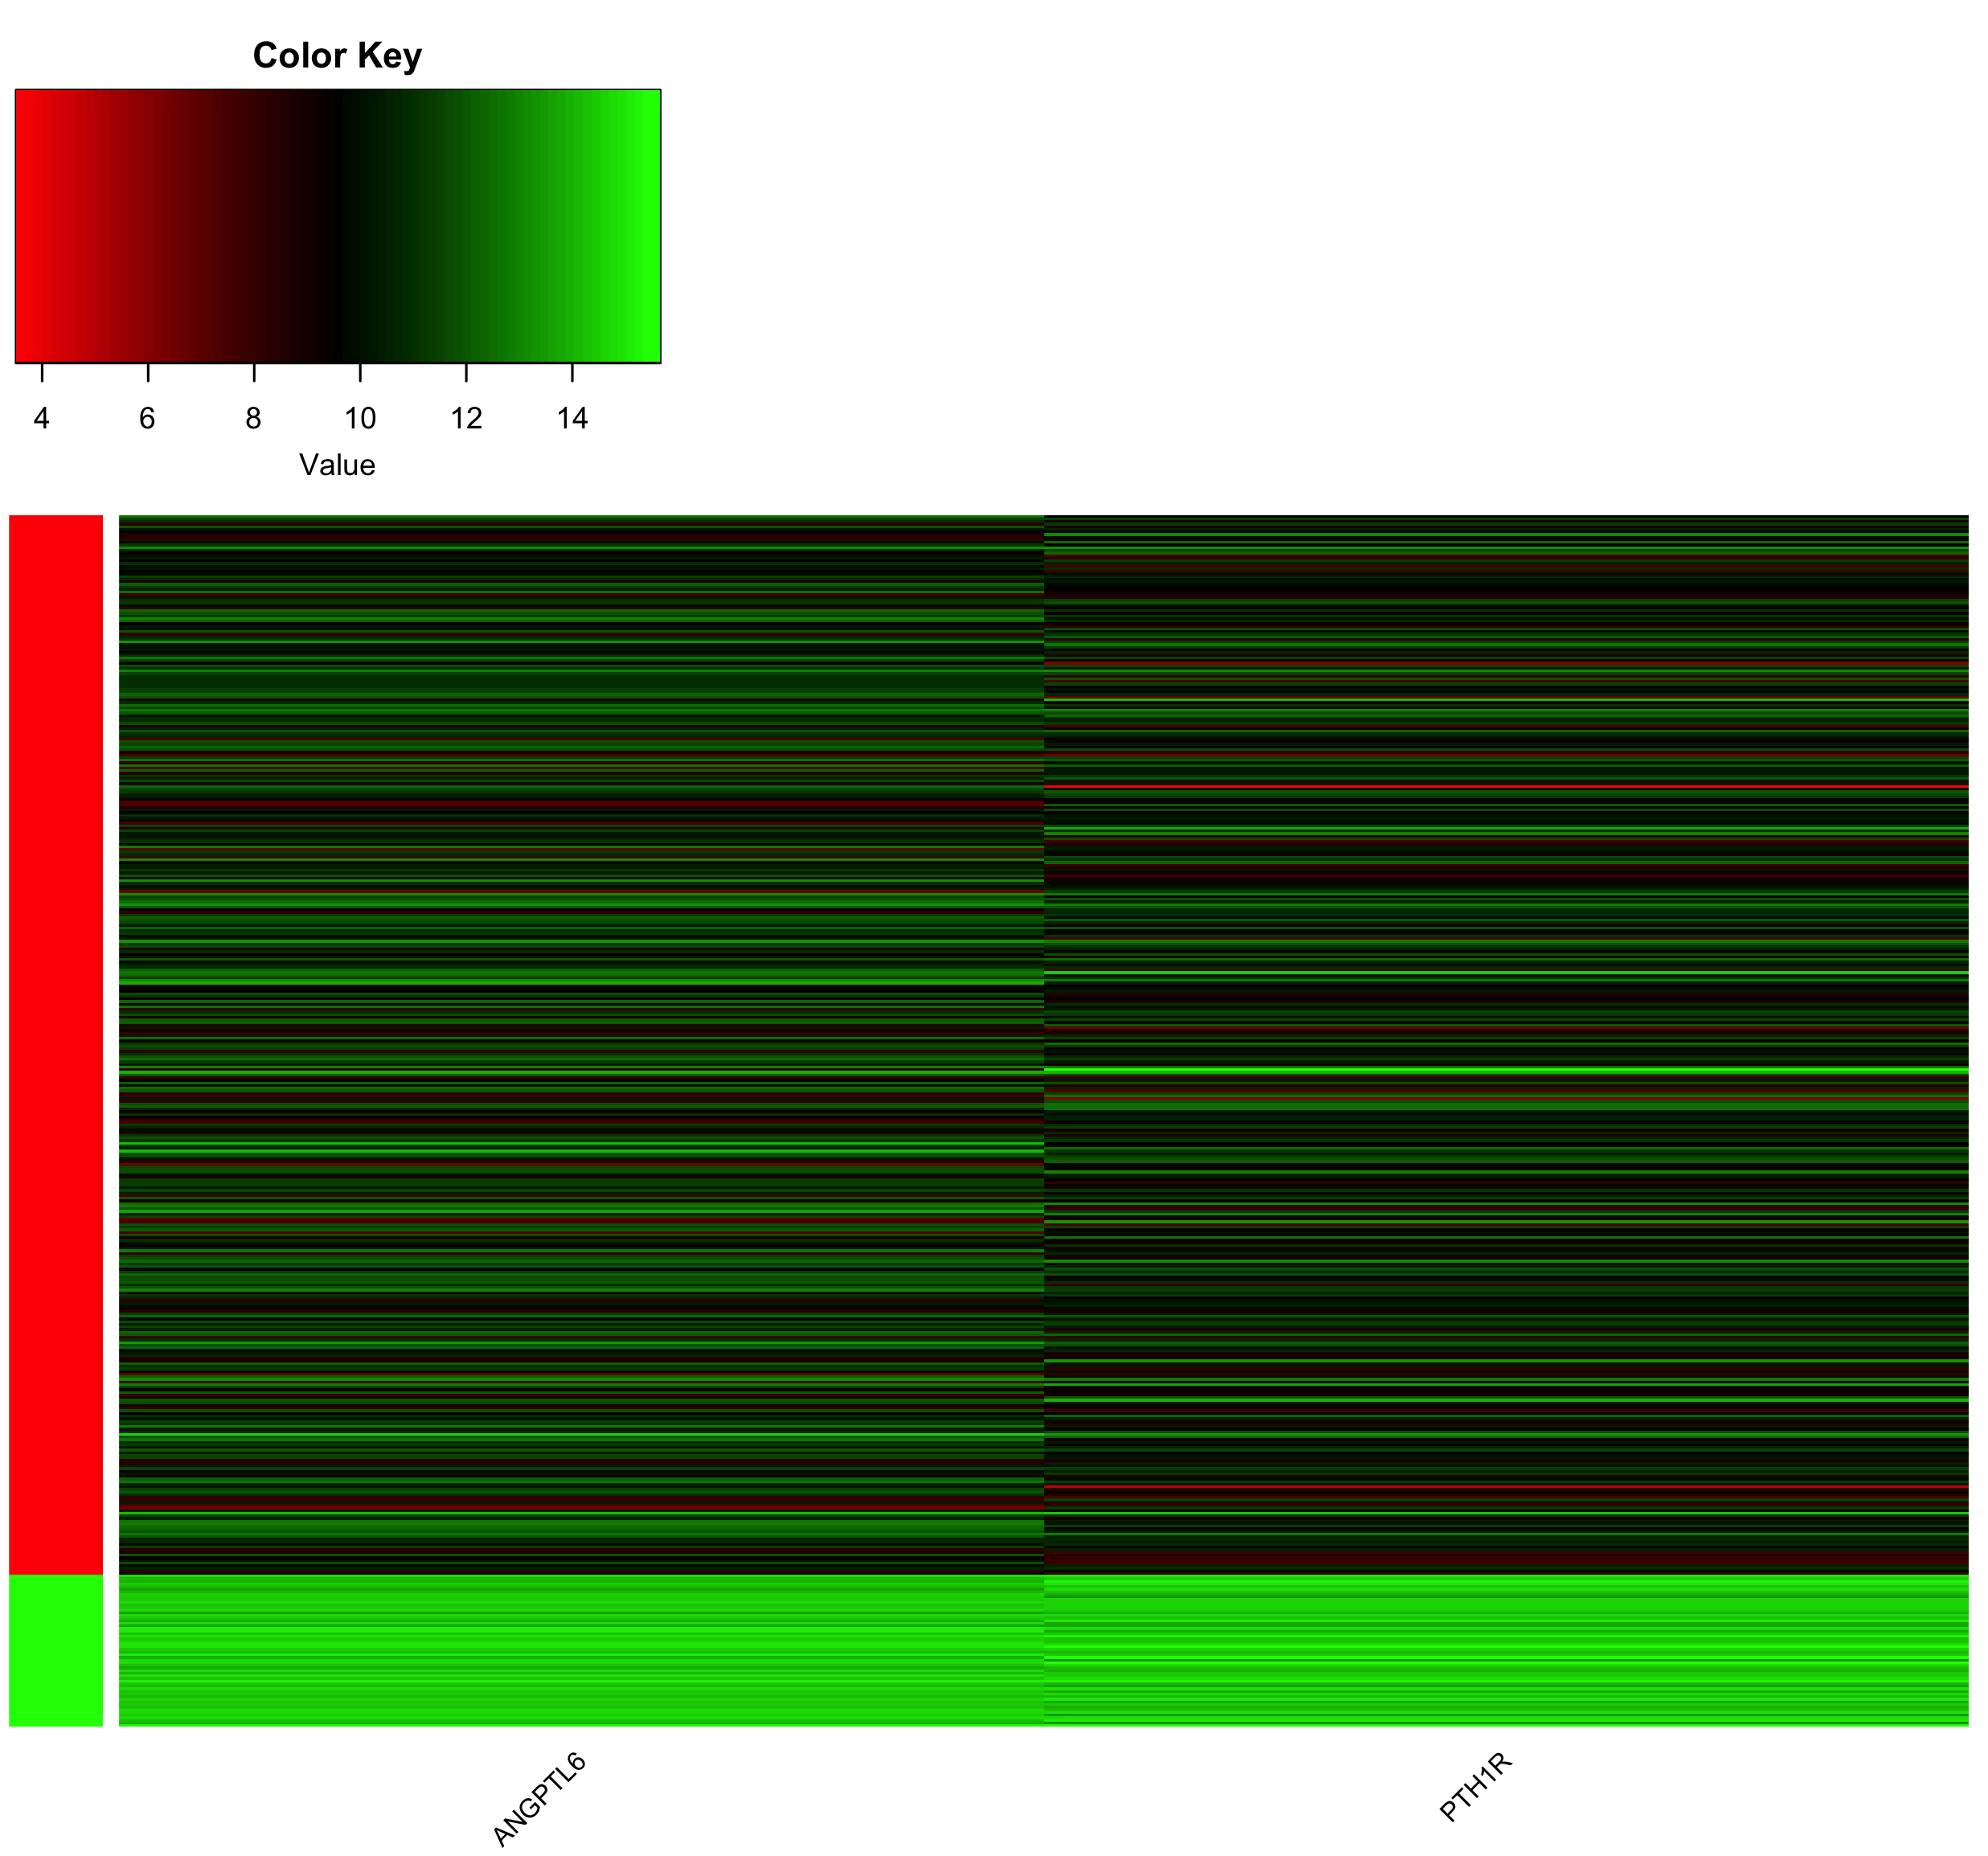
\includegraphics[width=1\textwidth]{figuras/15_higado_biclase_42_knn_heatmap_mejor_metodo.png} 
\end{center}

\newpage
\begin{center}
\textbf{Figura 16}. Diagrama de caja de expresión de genes por tipo de muestra en los 2 genes más relevantes encontrados en el mejor modelo de kNN con RF como método de selección de características.
\end{center}
\begin{center}
	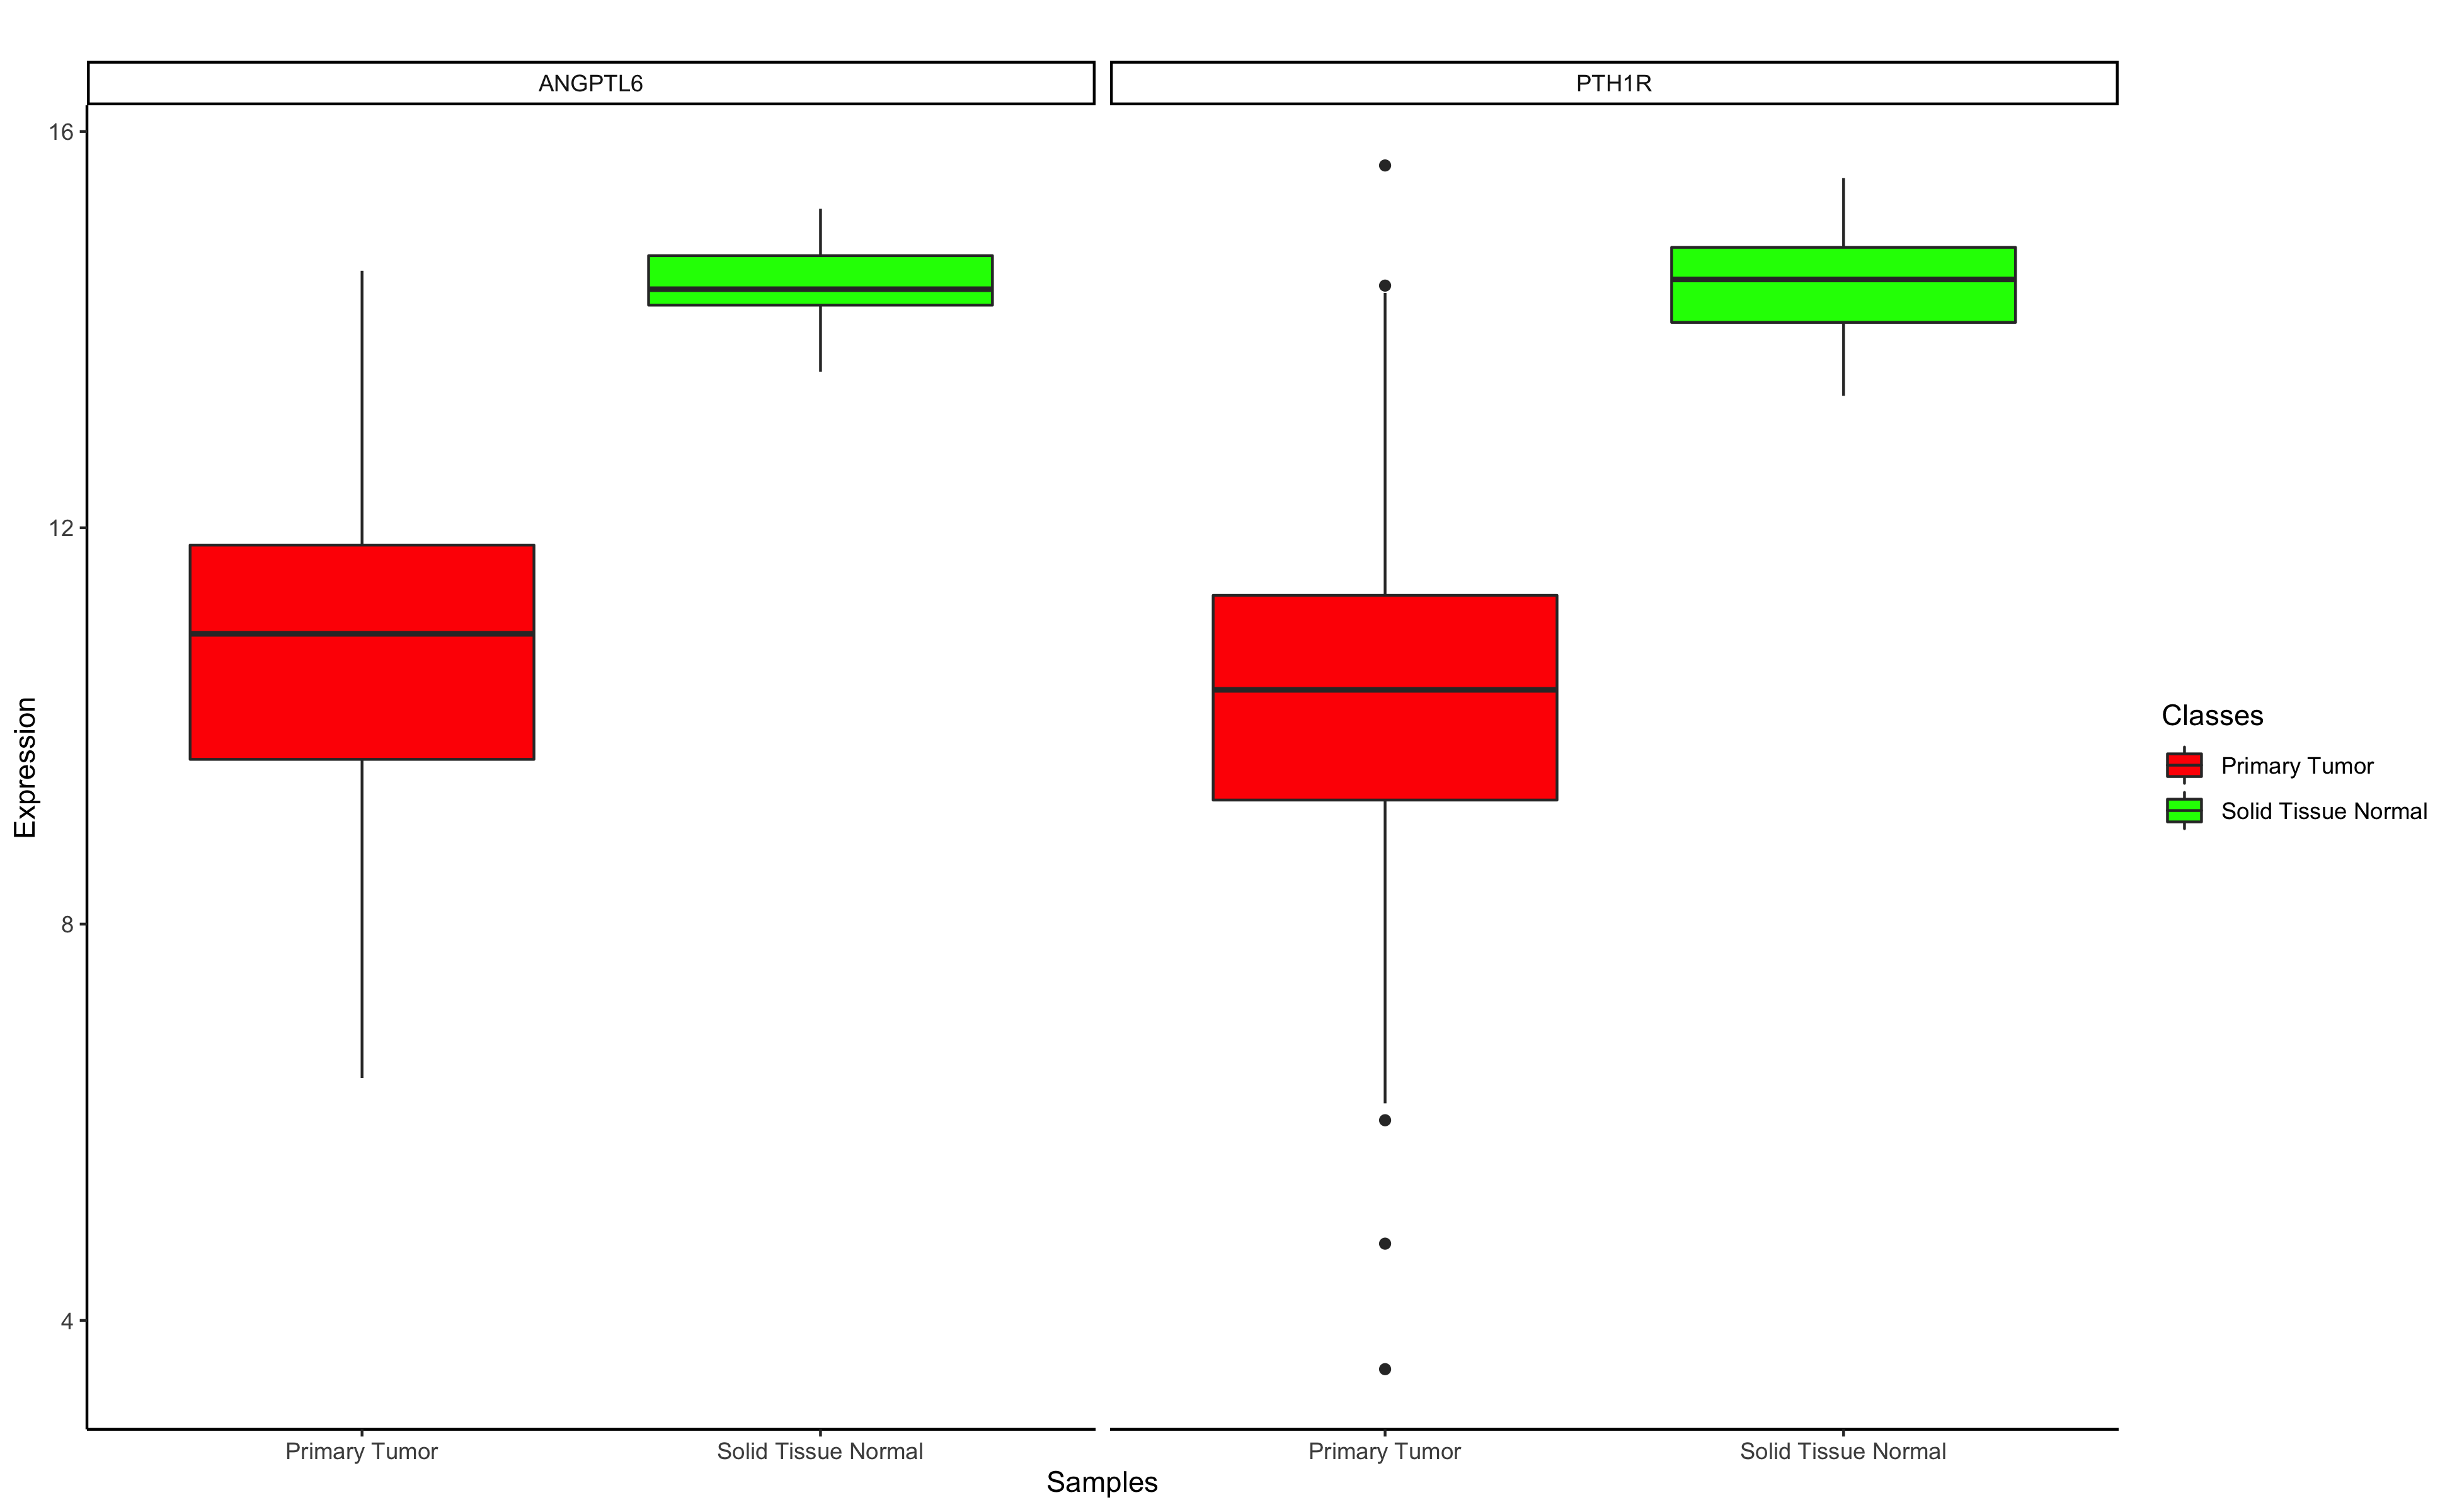
\includegraphics[width=1\textwidth]{figuras/16_higado_biclase_43_knn_boxplots_mejor_metodo.png} 
\end{center}

\subsection{Validación en test}

Al validar en el conjunto de test el mejor modelo encontrado para SVM (4 genes con RF), RF (7 genes con mRMR) y kNN (2 genes con RF) se obtiene la misma clasificación: una predicción perfecta a falta de un falso positivo, esto es, una muestra de tejido normal que ha sido clasificada como tumor. El F1-Score en test es de 99,5\% con una precisión de 99,1\%.

\newpage
\begin{center}
	\textbf{Figura 17}. Matriz de confusión de los mejores modelos encontrados de SVM, RF y kNN en el conjunto de test.
\end{center}

\begin{center}
	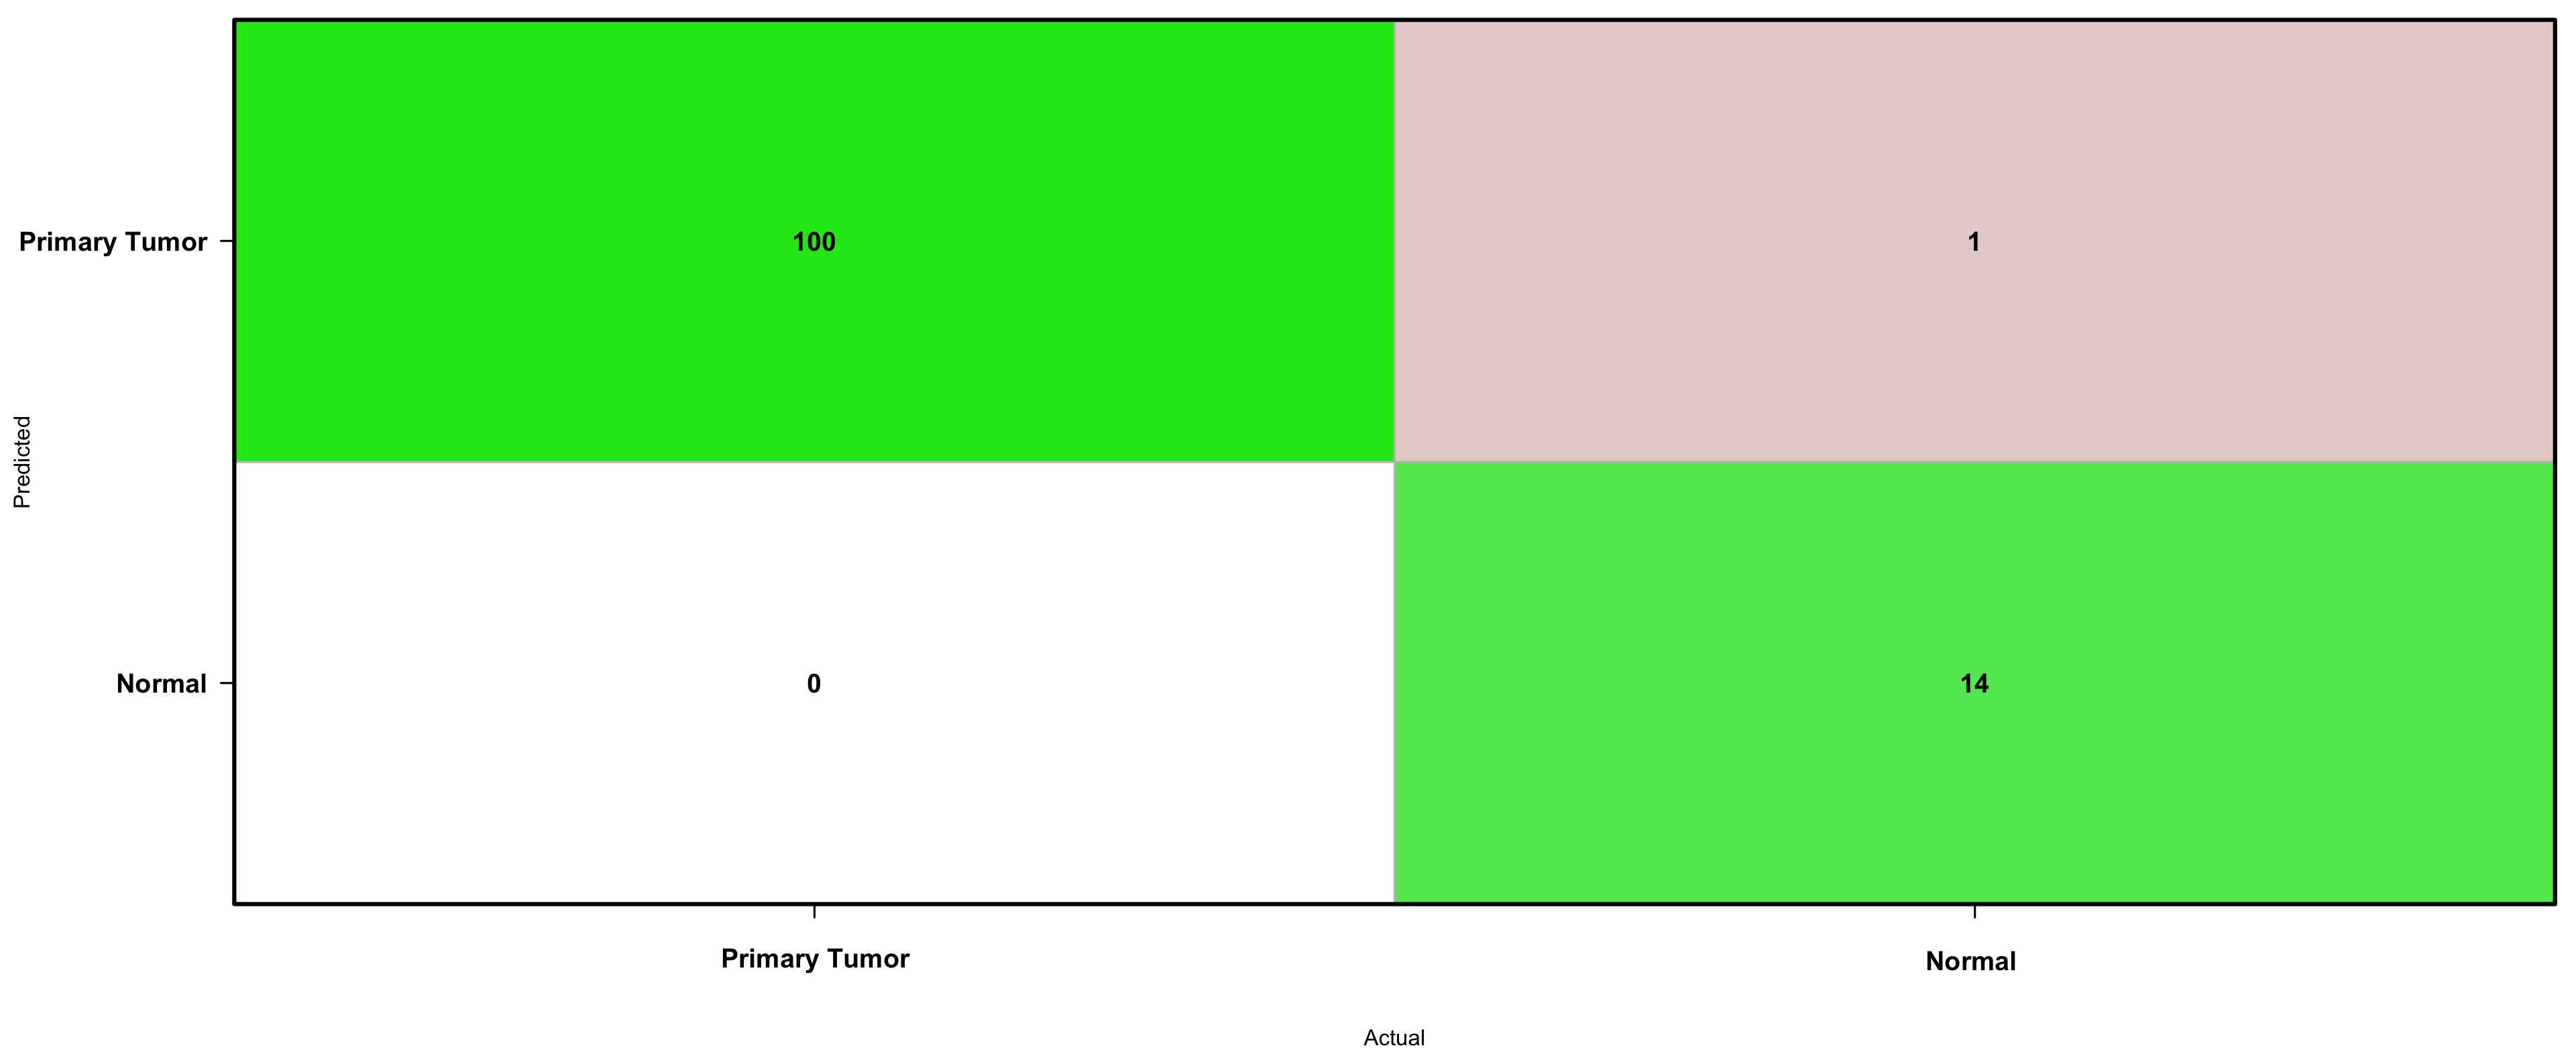
\includegraphics[width=1\textwidth]{figuras/17_higado_biclase_18_svm_matriz_confusion_mejor_metodo.png} 
\end{center}

En la Tabla 19 se muestra un resumen de los mejores modelos obtenidos y su F1-Score y precisión en conjunto de entrenamiento y conjunto de test.\\

\textbf{Tabla 19}. Resumen de clasificación biclase para cáncer de hígado. Mejor modelo encontrado para SVM, RF y kNN con biomarcadores seleccionados, parámetros optimizados para cada algoritmo, F1-Score y precisión (Acc) en conjunto de entrenamiento y conjunto de test.

\begin{table}[H]
	\centering
	\begin{tabular}{llccccc}
        \cline{2-7} 
		& Biomarcadores & Parámetros  & F1 train    & \multicolumn{1}{c|}{Acc train}      & F1 test       & Acc test       \\ \hline
		SVM & \textbf{4 genes} RF    & \begin{tabular}[c]{@{}c@{}}$c$ = 0.75\\ $\gamma$ = 0.1\end{tabular} & 99,67          & \multicolumn{1}{c|}{99,42}          & 99,5          & 99,13          \\ \hline
		RF  & \textbf{7 genes} mRMR & --                                                                  & 99,68 & \multicolumn{1}{c|}{99,43} & 99,5 & 99,13 \\ \hline
		kNN & \textbf{2 genes} RF    & $k$ = 5                                                             & 99,67          & \multicolumn{1}{c|}{99,42}          & 99,5          & 99,13          \\ \hline
	\end{tabular}
\end{table}

\subsection{Conclusiones}

Como conclusiones del presente experimento, los valores de F1-score y precisión son muy altos en la validación cruzada en entrenamiento, superando el 90\% en el mejor modelo de cada algoritmo. Es relevante destacar la alta eficiencia del modelo de kNN, que consigue grandes resultados usando únicamente 2 genes: ANGPTL6 y PTH1R. Estos dos genes son posibles biomarcadores diana debido su gran poder de discernimiento entre tejido tumoral y sano.\\

En la plataforma de Open Targets \cite{OpenTargets2020} no se encuentra ninguna asociación entre el gen ANGPTL6 y el cáncer de hígado, aunque está asociado con el cáncer \cite{Carbone2018} y la cirrosis biliar primaria \cite{Liu2012}. Para el gen PTH1R, se encuentran asociaciones con varios tipos de cáncer \cite{Michailidou2017, Michailidou2015} y algunos factores de riesgo del cáncer de hígado como el consumo de alcohol \cite{biobank} o padecer diabetes tipo II \cite{Xue2018}.\\

Todos los genes seleccionados por los mejores modelos tienen relación con el cáncer. Los genes CCNE1
y CDH13 están directamente relacionados con el cáncer de hígado, y los genes ANGPTL6, ADAMTS13, BMPER, CCNE1
y CDH13 están relacionados con distintas enfermedades hepáticas.

\section{Resultados de clasificación multiclase para cáncer de hígado}

El código completo del análisis se muestra en el fichero \textit{\texttt{analisis\_higado/\linebreak04\_analisis\_multiclase.R}} del repositorio de GitHub asociado al trabajo \cite{Redondo-Sanchez2020}.

\subsection{Detección de biomarcadores}

Para la clasificación multiclase en cáncer de hígado se van a considerar los dos principales tipos de diagnósticos primarios presentes en los datos clínicos de cáncer de hígado: carcinoma hepatocelular y colangiocarcinoma. Se excluyen los tumores con otros diagnósticos primarios (8 casos). En la Tabla 20 se muestra la distribución de muestras.\\

\textbf{Tabla 20}. Distribución de tipos de muestra para el análisis de cáncer de hígado multiclase.

\begin{table}[H]
	\centering
	\begin{tabular}{lcc}
		\cline{2-3}
		& \textbf{Número de casos} & \textbf{Porcentaje} \\ \hline
		\textbf{Carcinoma hepatocelular}     & 363        & 80,0\%              \\
		\textbf{Colangiocarcinoma}     & 33        & 7,3\%              \\
		\textbf{Tejido sano} & 58         & 12,8\%              \\ \hline
		\textbf{Total}       & 454        & 100\%               \\ \hline
	\end{tabular}
\end{table}

Se extraen 8.533 genes que presentan en su expresión diferencias significativas entre las muestras de tumores y las de tejido sano. En la Tabla 21 se muestra la partición entrenamiento - test realizada y en la Figura 18 se representa en un diagrama de Sankey.\\

\textbf{Tabla 21}. Distribución entrenamiento-test según tipo de muestra y proporción entre clases para el análisis de hígado multiclase.\\

\begin{table}[H]
	\centering
\begin{tabular}{lccc}
	\cline{2-4}
	\multicolumn{1}{c}{\textbf{}}                                                    & \textbf{Total} & \textbf{Entrenamiento} & \textbf{Test} \\ \hline
	\textbf{Carcinoma hepatocelular}                                                 & 363 (100\%)    & 273 (75,2\%)           & 90 (24,8\%)   \\
	\textbf{Colangiocarcinoma}                                                       & 33 (100\%)     & 25 (75,8\%)            & 8 (24,2\%)    \\
	\textbf{Tejido sano}                                                             & 58 (100\%)     & 44 (75,9\%)            & 14 (24,1\%)   \\ \hline
	\textbf{\begin{tabular}[c]{@{}l@{}}Proporción\\ carc. hepat./sanos\end{tabular}} & 6,3            & 6,2                    & 6,4           \\
	\textbf{\begin{tabular}[c]{@{}l@{}}Proporción\\ colang./sanos\end{tabular}}      & 0,6            & 0,6                    & 0,6           \\ \hline
\end{tabular}
\end{table}

\begin{center}
\textbf{Figura 18}. Diagrama de Sankey mostrando la partición entrenamiento-test realizada según tipo de muestra para el análisis de hígado multiclase.
\end{center}
\begin{center}
	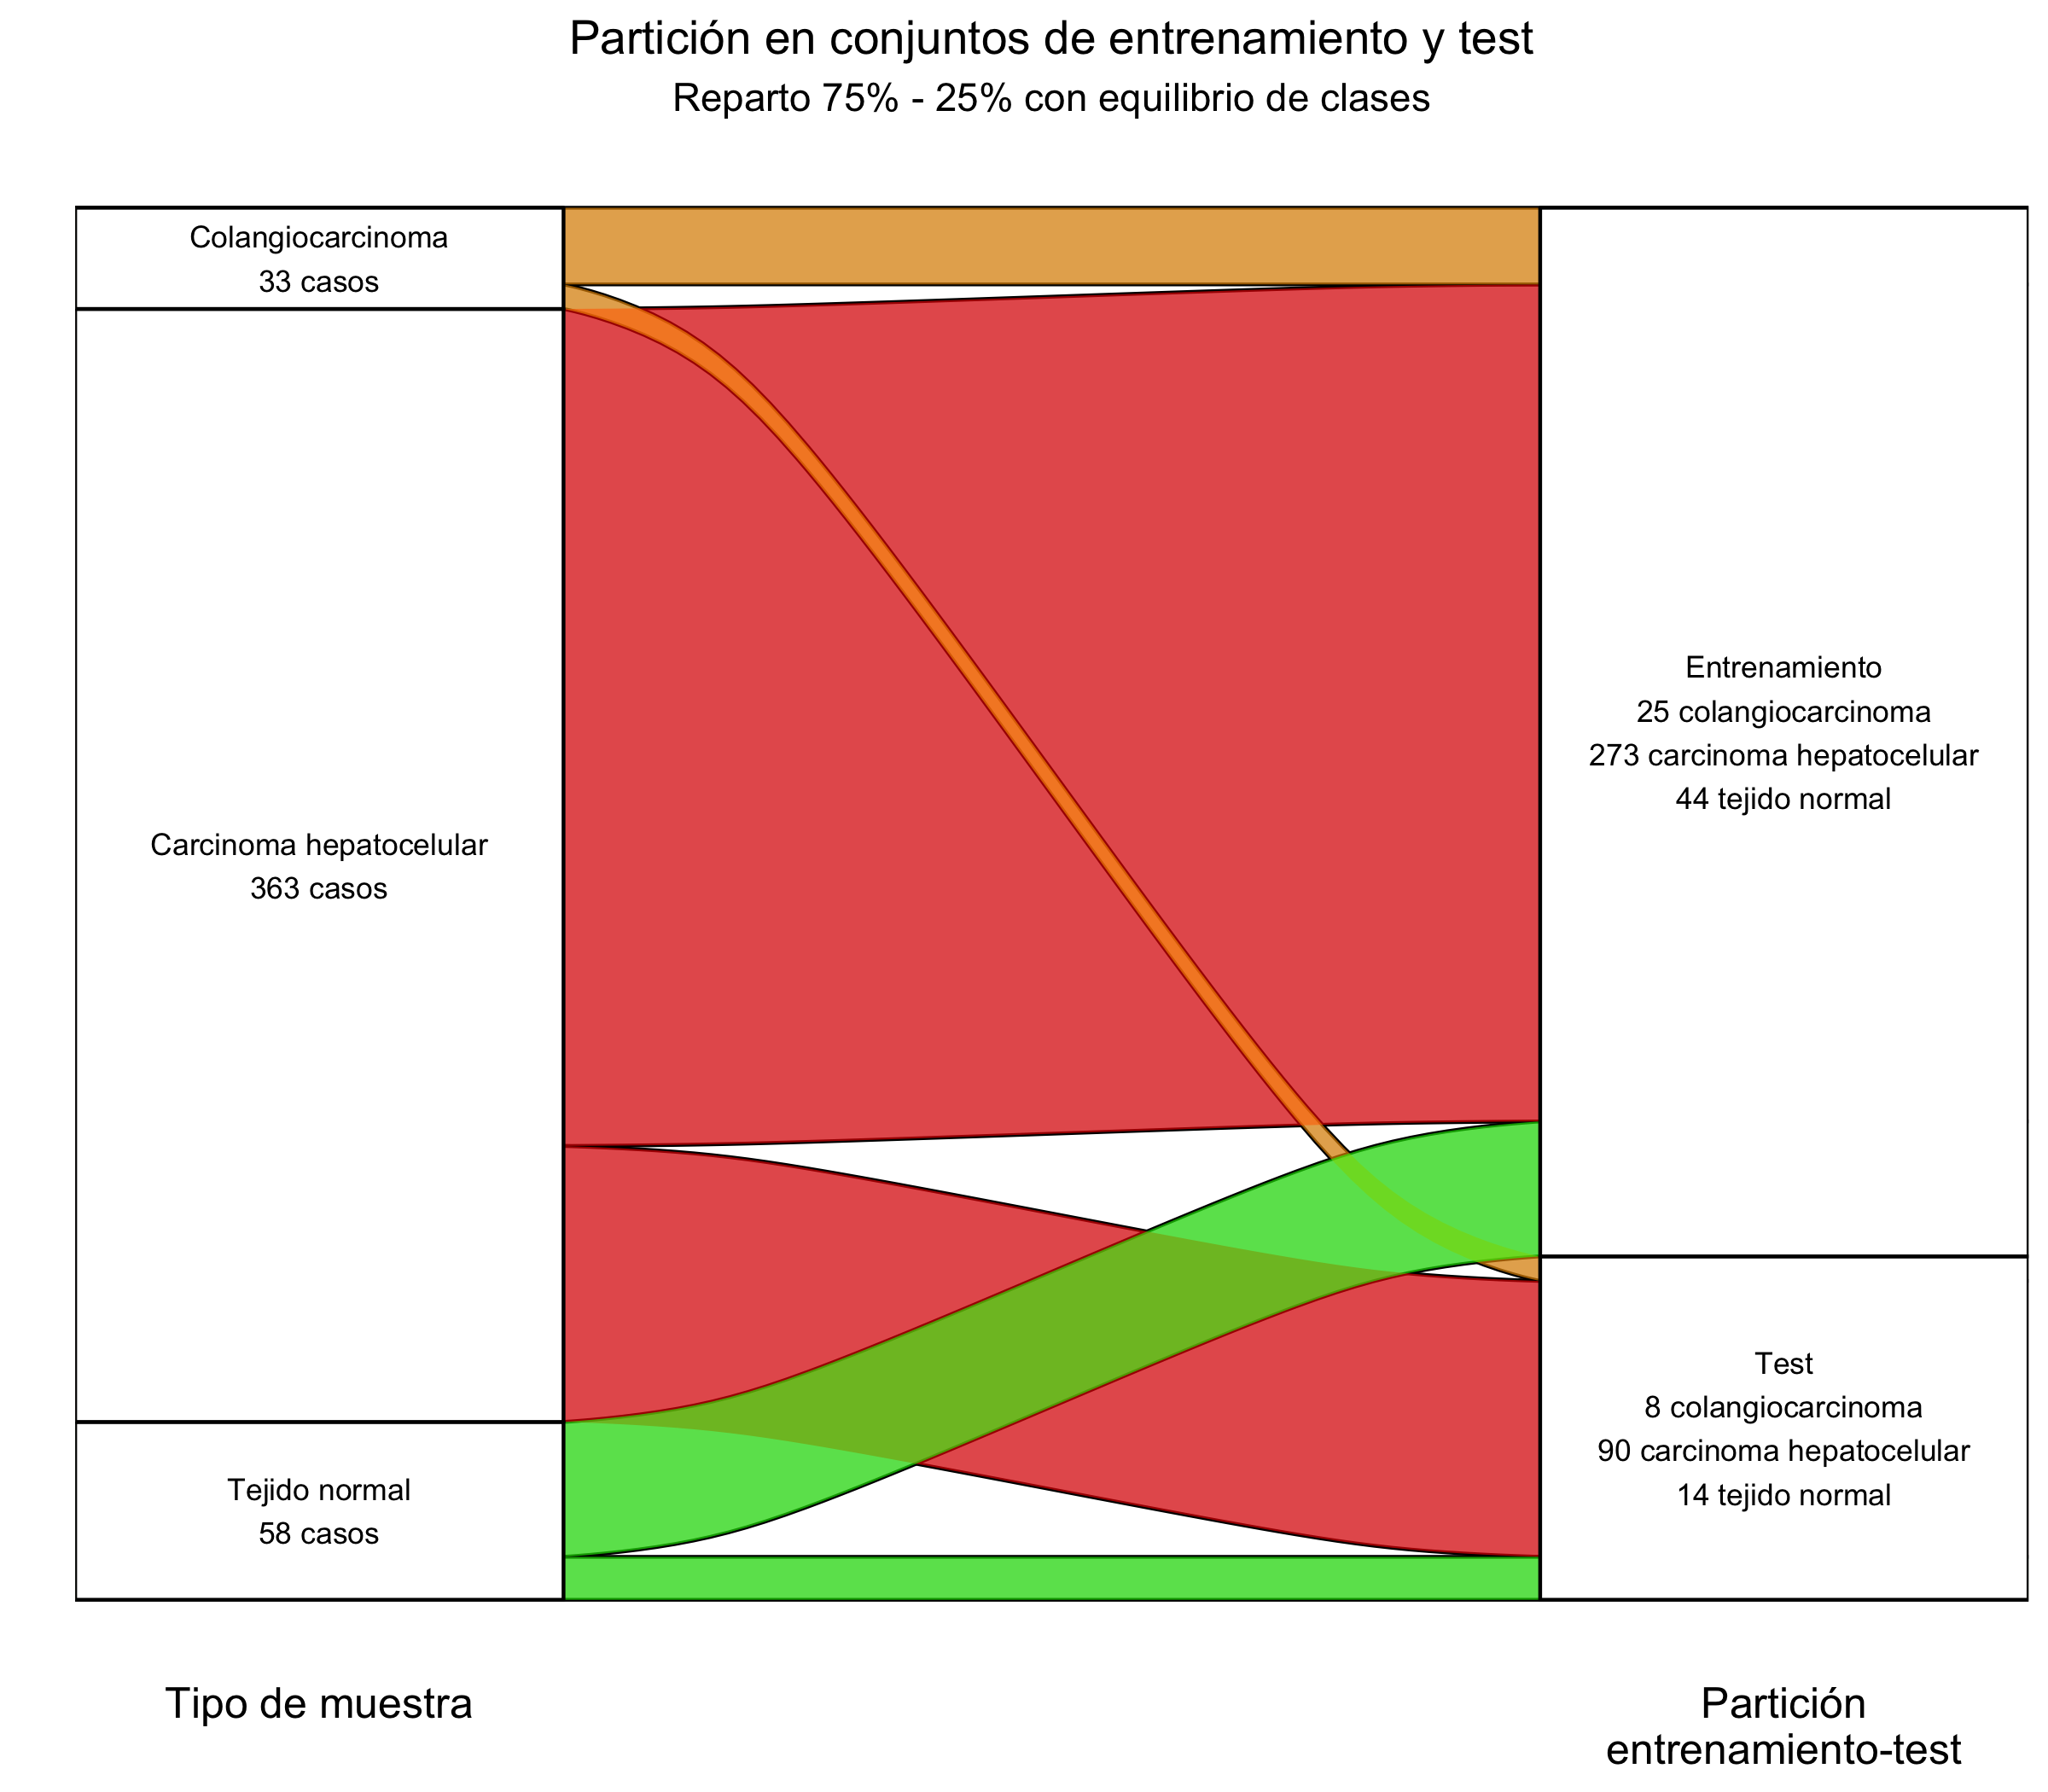
\includegraphics[width=.75\textwidth]{figuras/18_higado_multiclase_05_sankey.png}
\end{center}

A continuación se muestran los diez genes más relevantes encontrados por cada método de selección de características:\\

\newpage
\textbf{Tabla 22}. Diez genes más relevantes según los distintos métodos de selección de características para el análisis de hígado multiclase.

\begin{table}[H]
	\centering
	\begin{tabular}{cccc}
		\hline
		\textbf{Ranking} & \multicolumn{1}{c}{\textbf{mRMR}} & \multicolumn{1}{c}{\textbf{RF}} & \multicolumn{1}{c}{\textbf{DA}} \\ \hline
		1                & ANGPTL6                           & ANGPTL6                         & WWTR1                           \\
		2                & FTLP3                             & GABRD                           & BIRC3                           \\
		3                & PLXDC1                            & CDH13                           & CDH1                            \\
		4                & RAB25                             & STAB2                           & ROS1                            \\
		5                & WDR66                             & BMPER                           & POLQ                            \\
		6                & AP2B1                             & ECM1                            & FGFR2                           \\
		7                & CDH13                             & ADAMTS13                        & KLF6                            \\
		8                & PTPN13                            & GDF2                            & CBFB                            \\
		9                & SLC31A1                           & CLEC4G                          & FGFR3                           \\
		10               & ADAMTS13                          & SPDL1                           & CLTCL1                          \\ \hline
	\end{tabular}
\end{table}

Se observa que tres genes han sido valorados como relevantes para los algoritmos de mRMR y RF:  ANGPTL6, CDH13 y ADAMTS13.

\subsection{Validación cruzada en entrenamiento - SVM}

En la Tabla 23 se muestran los parámetros óptimos de SVM obtenidos tras la búsqueda en rejilla.\\

\textbf{Tabla 23}. Parámetros óptimos de SVM encontrados para los 10 genes más relevantes de cada método de selección de características.

\begin{table}[H]
	\centering
	\begin{tabular}{cccc}
		\hline
		\textbf{Parámetro} & \textbf{mRMR} & \textbf{RF} & \textbf{DA} \\ \hline
		Coste                &    1 &    5     &   2       \\
		Gamma               &     0,025    &     0,08   & 0,02        \\ \hline
	\end{tabular}
\end{table}

Para estos parámetros óptimos, en la Figura 19 se muestran las medidas de evaluación medias obtenidas en las 5 fold.\\

\newpage
\begin{center}
\textbf{Figura 19}. Mapa de calor con valores medios y desviación típica de los 5-fold de F1-Score, precisión, sensibilidad y especificidad de SVM según método de selección de características y número de genes usados.
\end{center}
\begin{center}
	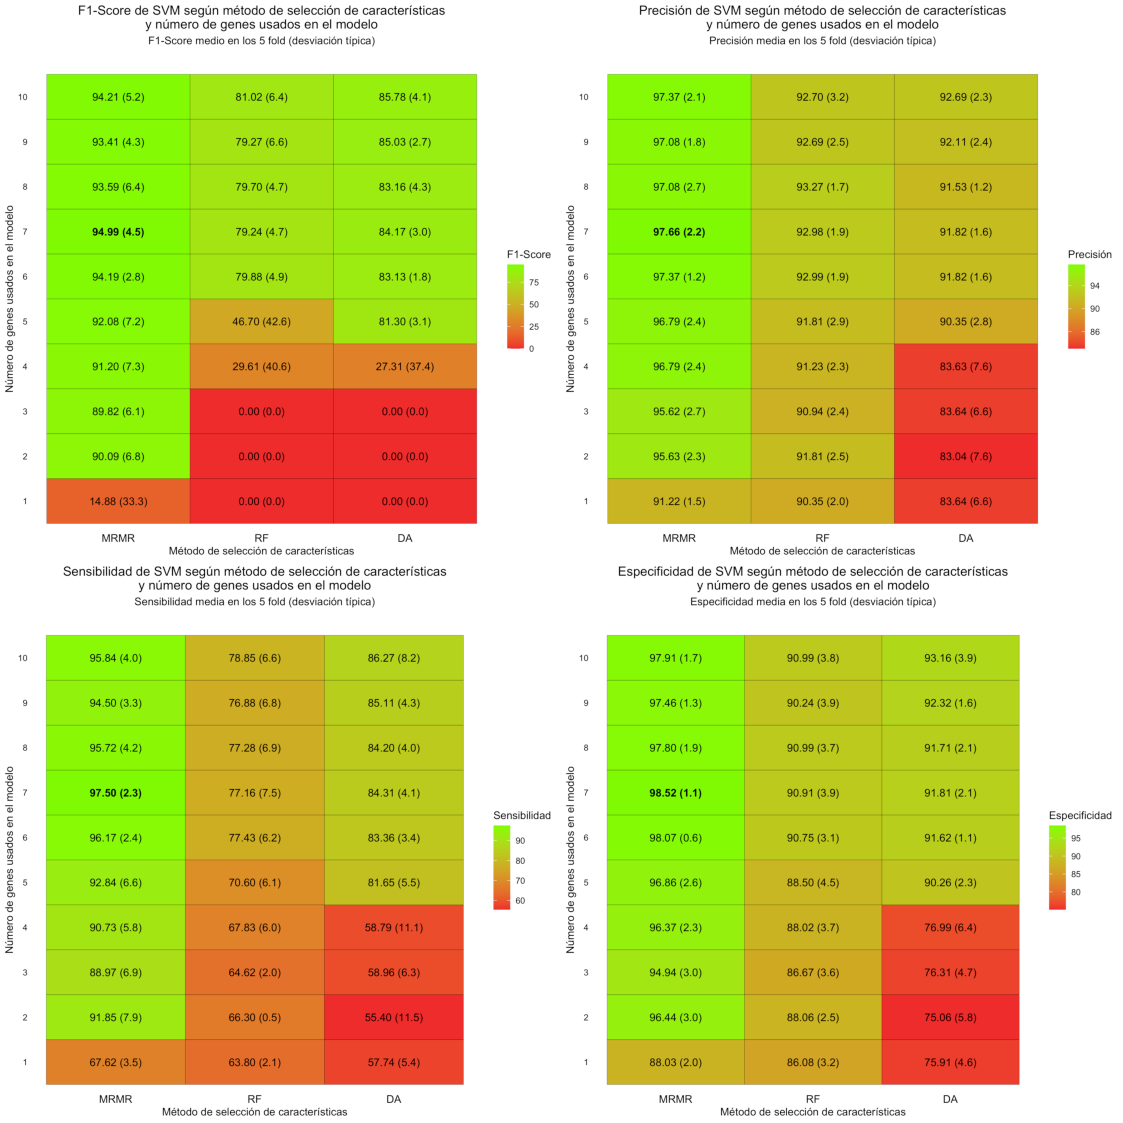
\includegraphics[width=1\textwidth]{figuras/19_higado_multiclase_heatmap_svm.pdf} 
\end{center}

El mejor F1-Score para SVM se obtiene con 7 genes seleccionados con mRMR (94,99\%), configuración que obtiene también los mejores valores de precisión (97,66\%), sensibilidad (97,50\%) y especificidad (98,52\%). Los 7 genes seleccionados son: ANGPTL6, FTLP3, PLXDC1, RAB25, WDR66, AP2B1 y CDH13. Se analiza la expresión de genes de estos 7 genes, utilizando para ello un mapa de calor (Figura 20) y diagramas de caja (Figura 21).

\newpage
\begin{center}
\textbf{Figura 20}. Mapa de calor de expresión de genes por tipo de muestra (columna izquierda: rojo = carcinoma hepatocelular, naranja = colangiocarcinoma, verde = tejido sano) en los 4 genes más relevantes encontrados en el mejor modelo de SVM con RF como método de selección de características.
\end{center}
\begin{center}
	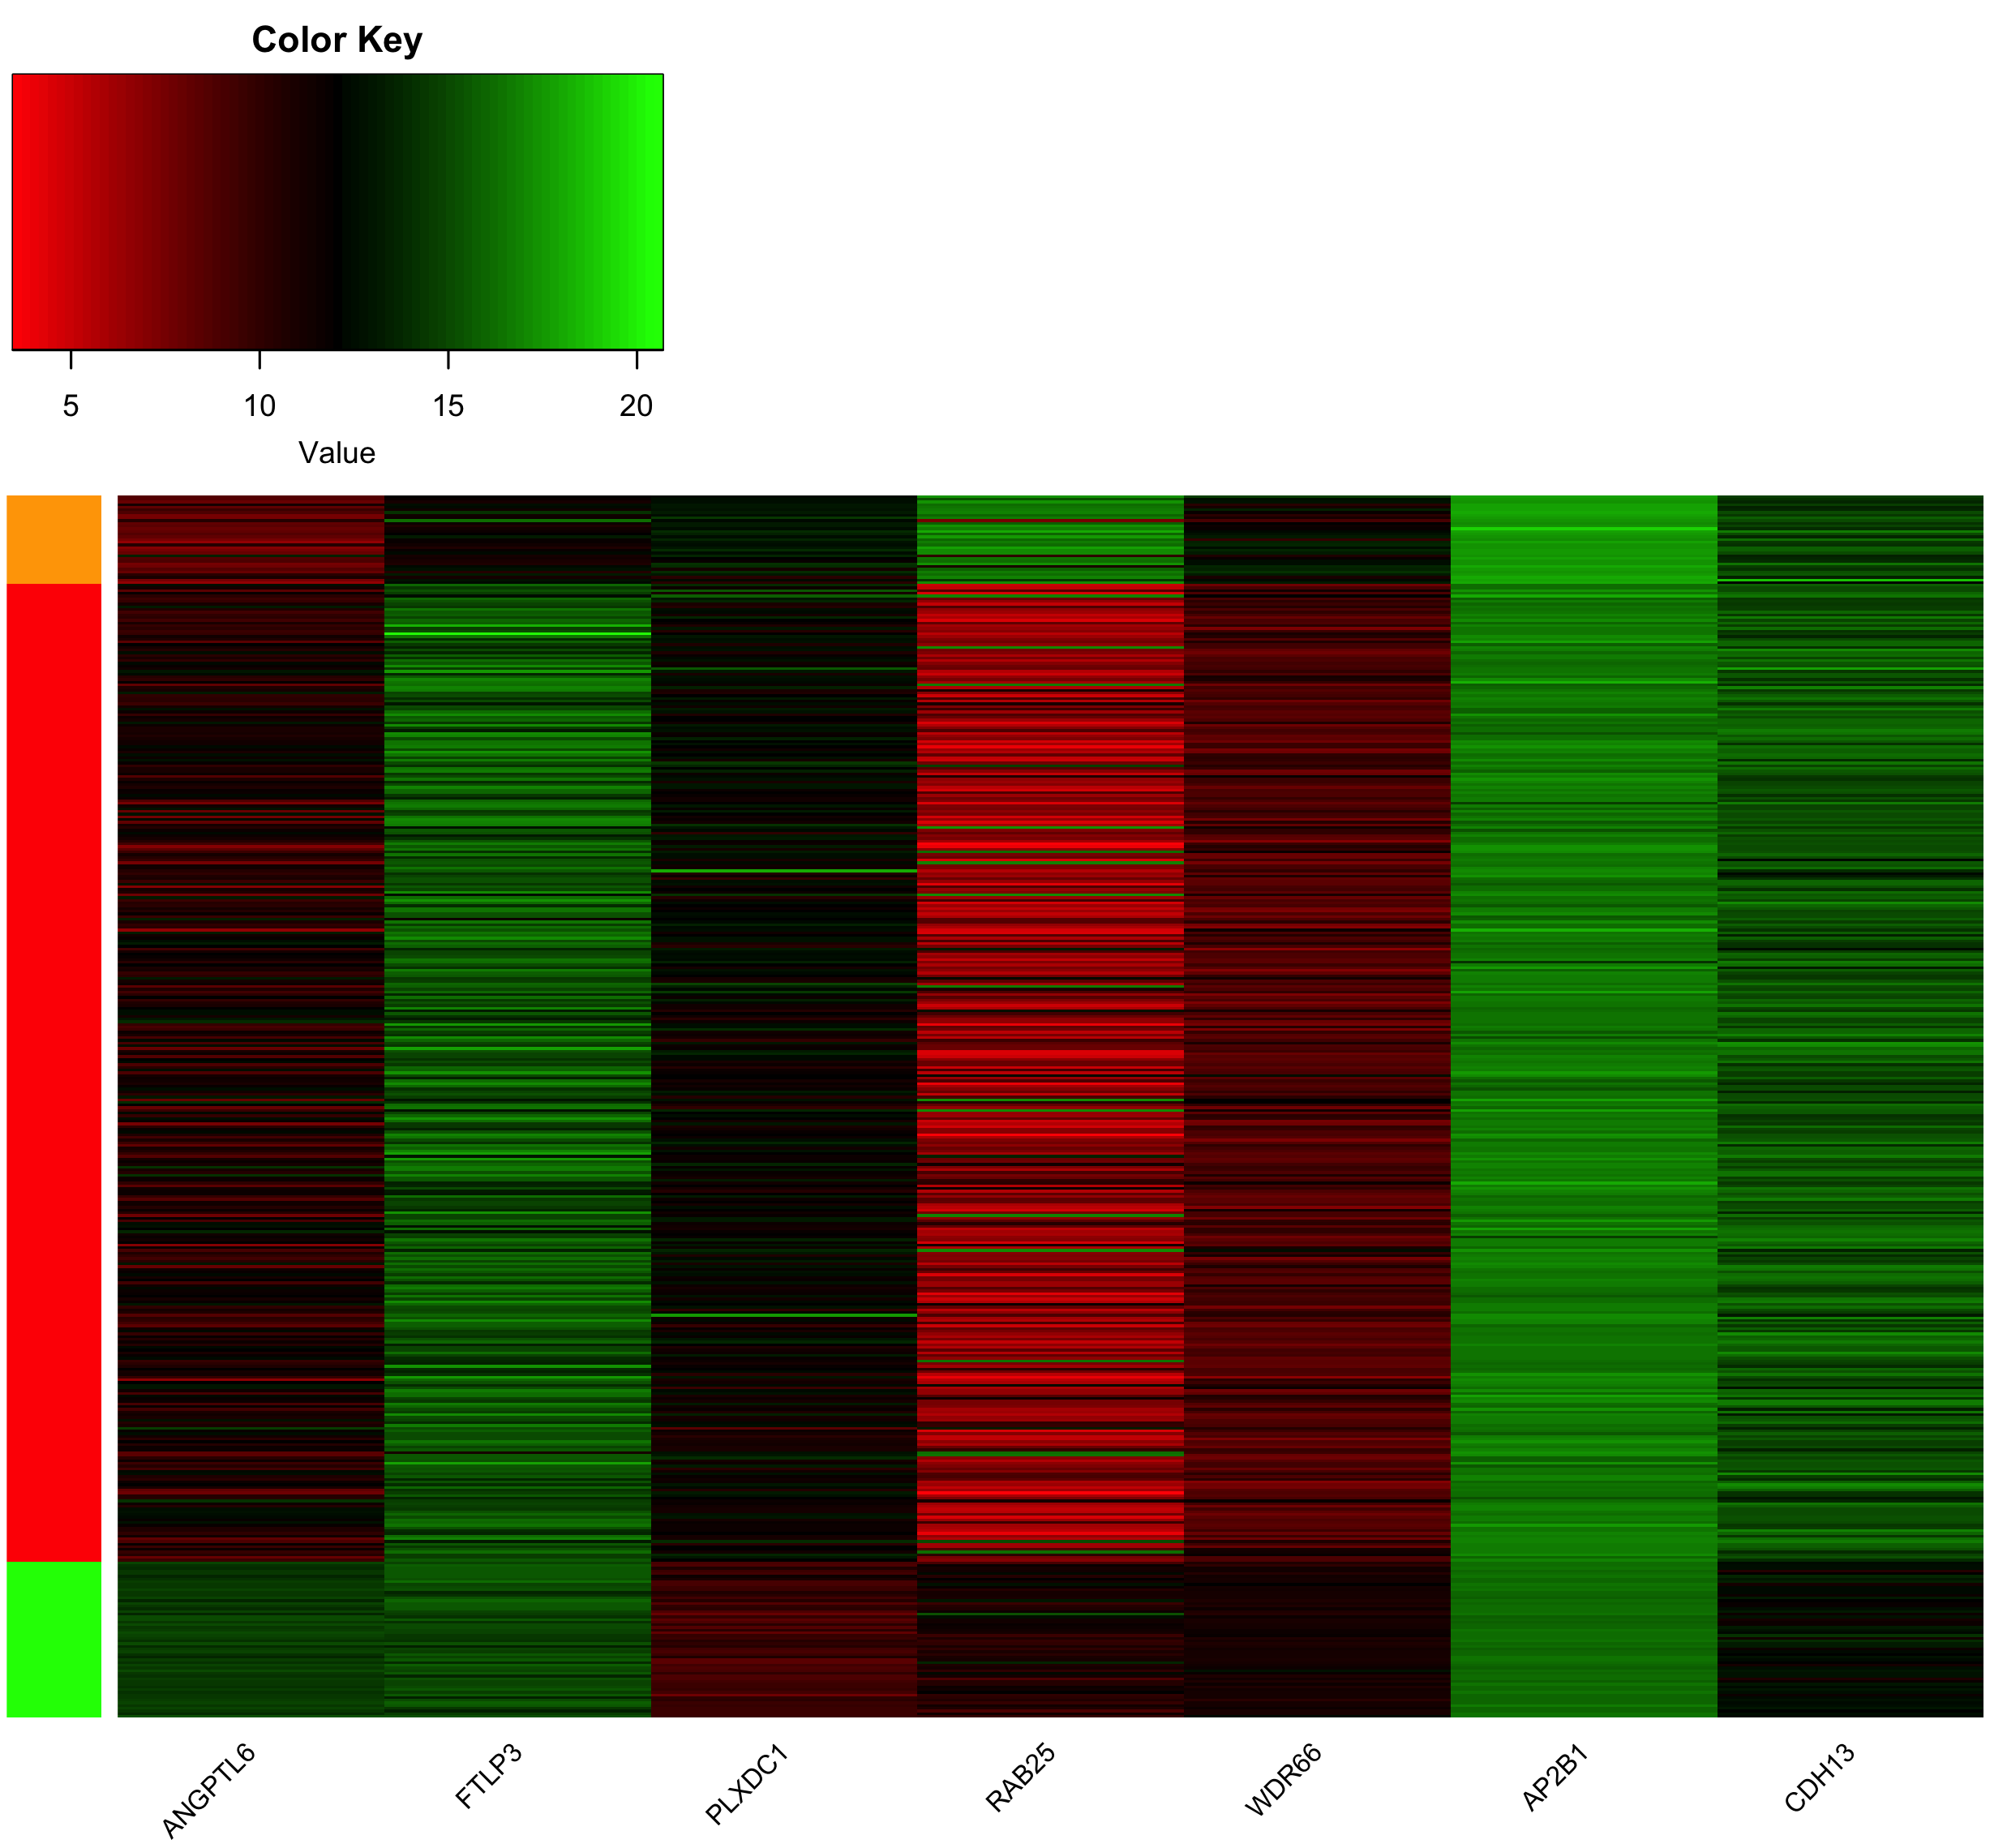
\includegraphics[width=1\textwidth]{figuras/20_higado_multiclase_13_svm_heatmap_mejor_metodo.png} 
\end{center}

En el mapa de calor se observa que hay grandes diferencias entre la expresión de genes de los distintos tipos de tejidos.

\newpage
\begin{center}
\textbf{Figura 21}. Diagrama de caja de expresión de genes por tipo de muestra en los 4 genes más relevantes encontrados en el mejor modelo de SVM con RF como método de selección de características.
\end{center}
\begin{center}
	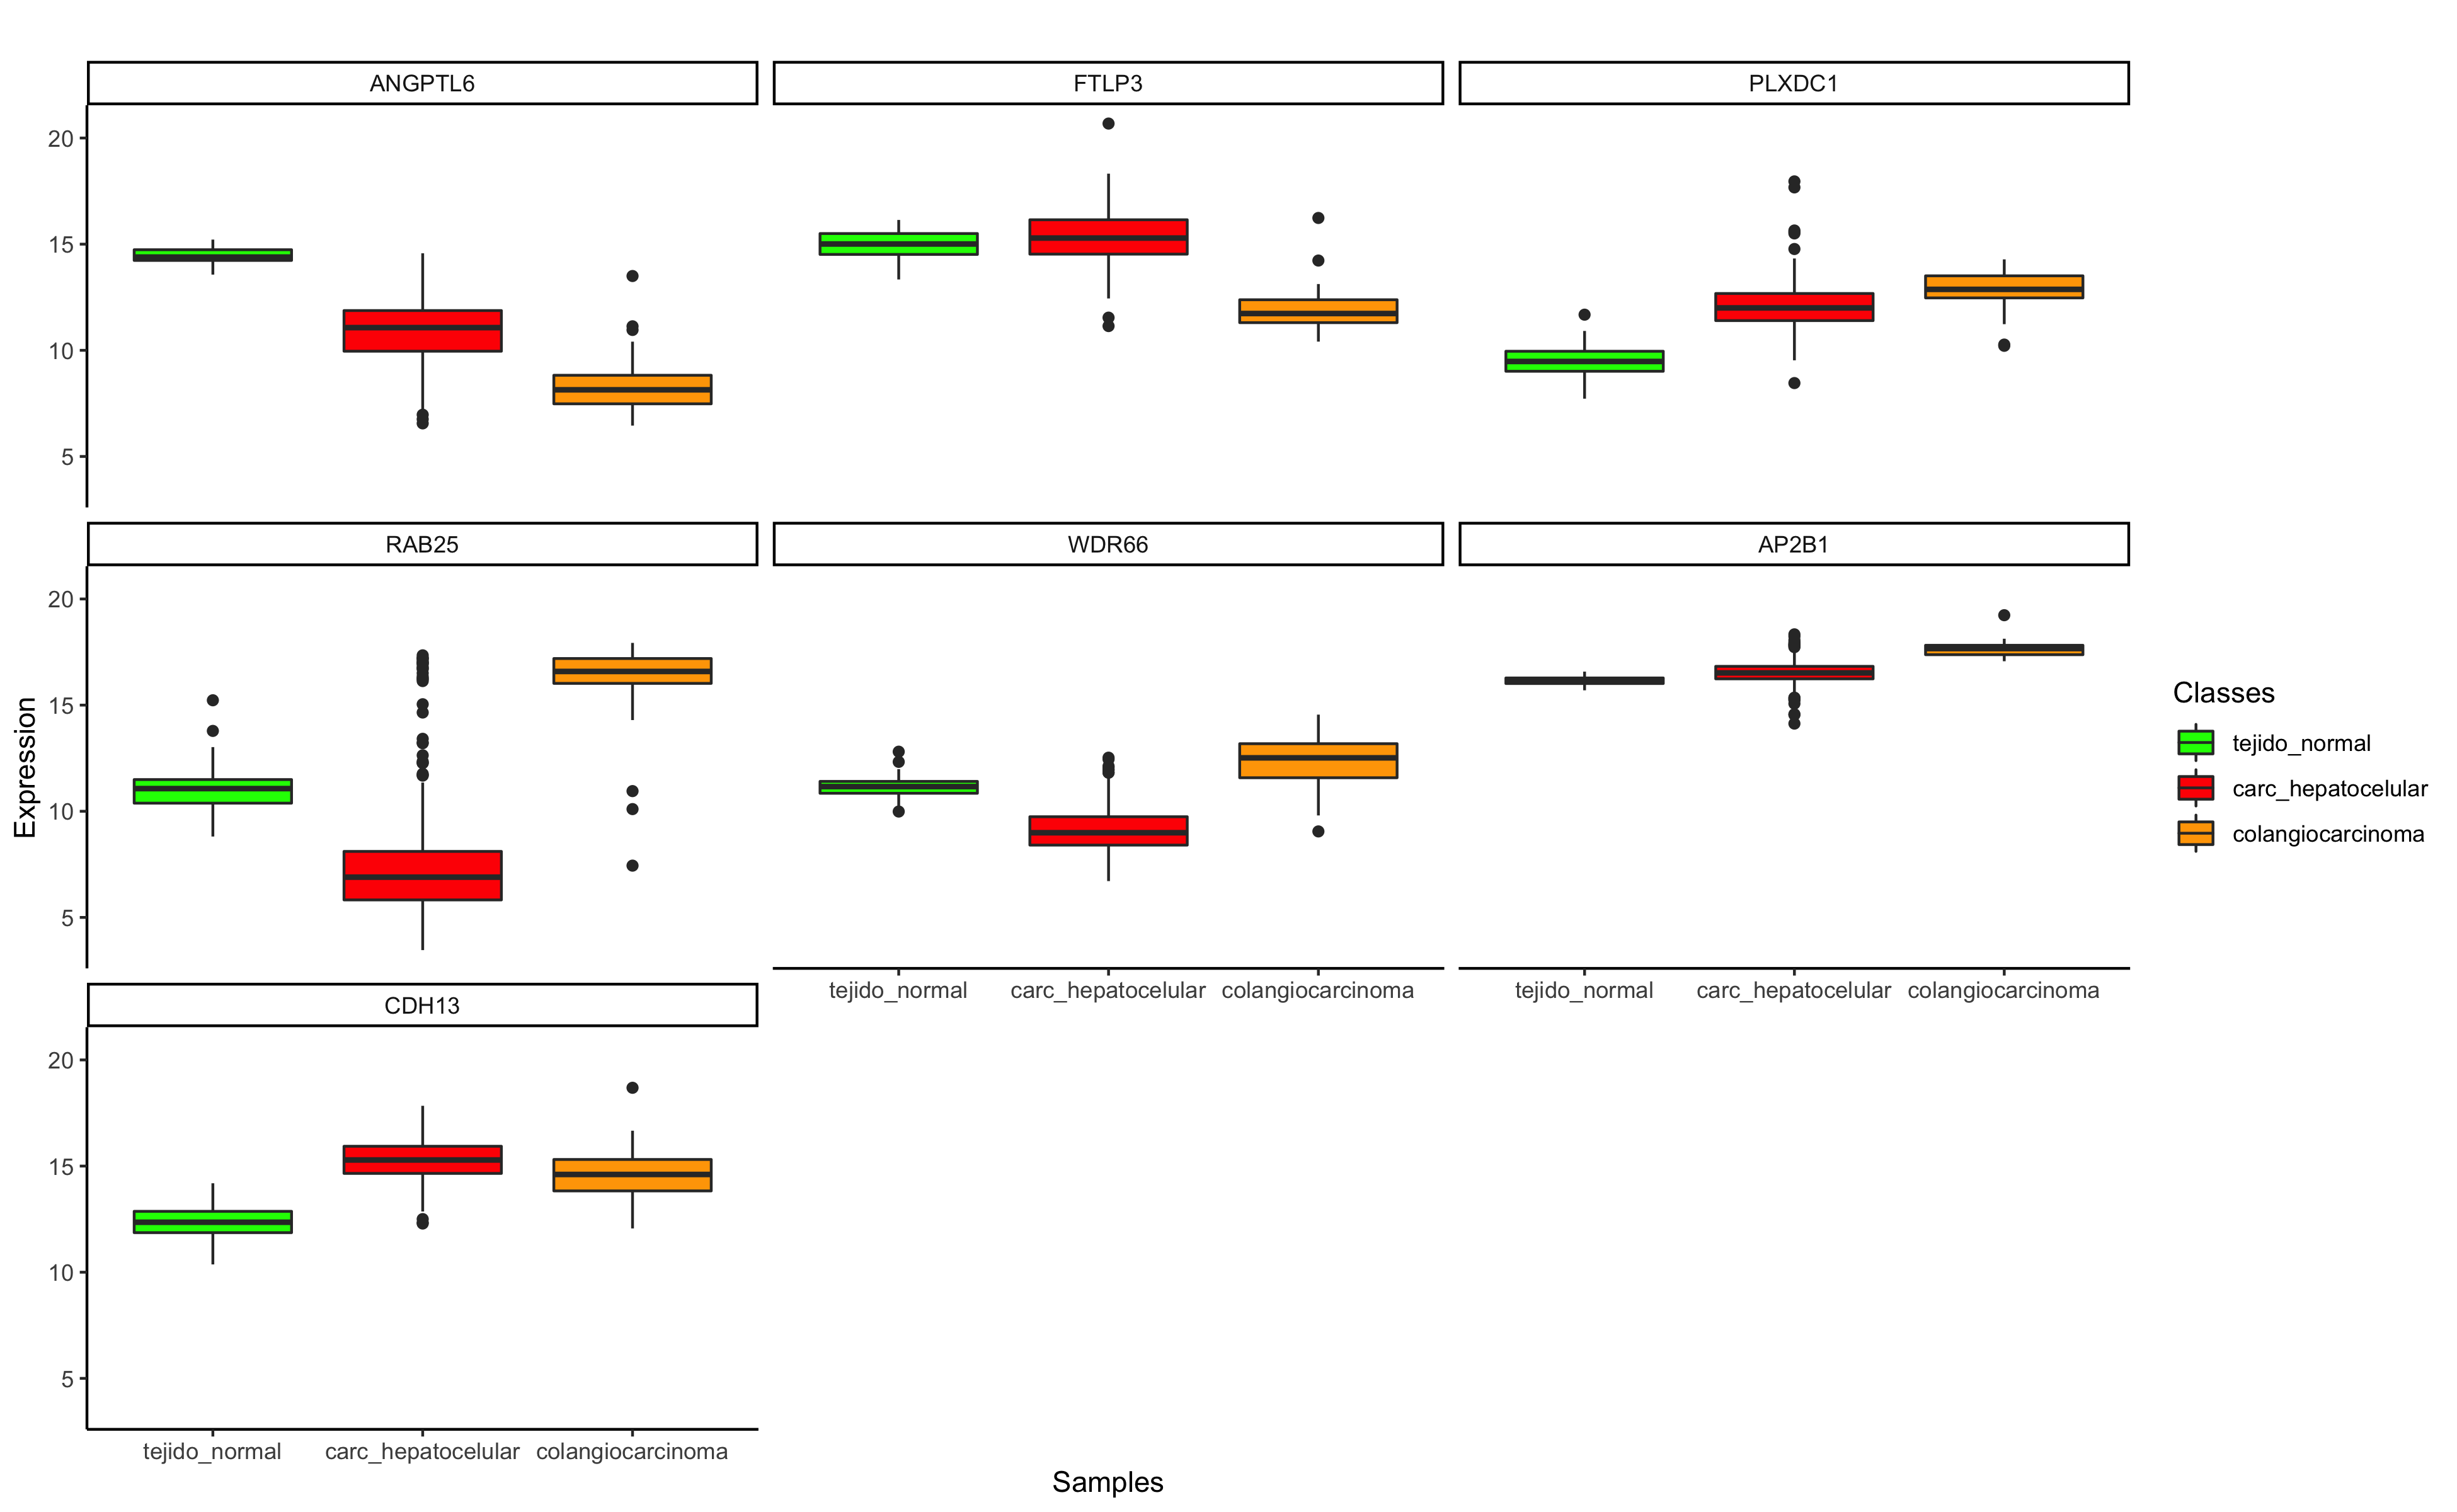
\includegraphics[width=1\textwidth]{figuras/21_higado_multiclase_14_svm_boxplots_mejor_metodo.png} 
\end{center}

\subsection{Validación cruzada en entrenamiento - RF}

En la Figura 22 se muestran las medidas de evaluación medias obtenidas en las 5 fold.\\

\newpage

\begin{center}
\textbf{Figura 22}. Mapa de calor con valores medios y desviación típica de los 5-fold de F1-Score, precisión, sensibilidad y especificidad de RF según método de selección de características y número de genes usados.
\end{center}
\begin{center}
	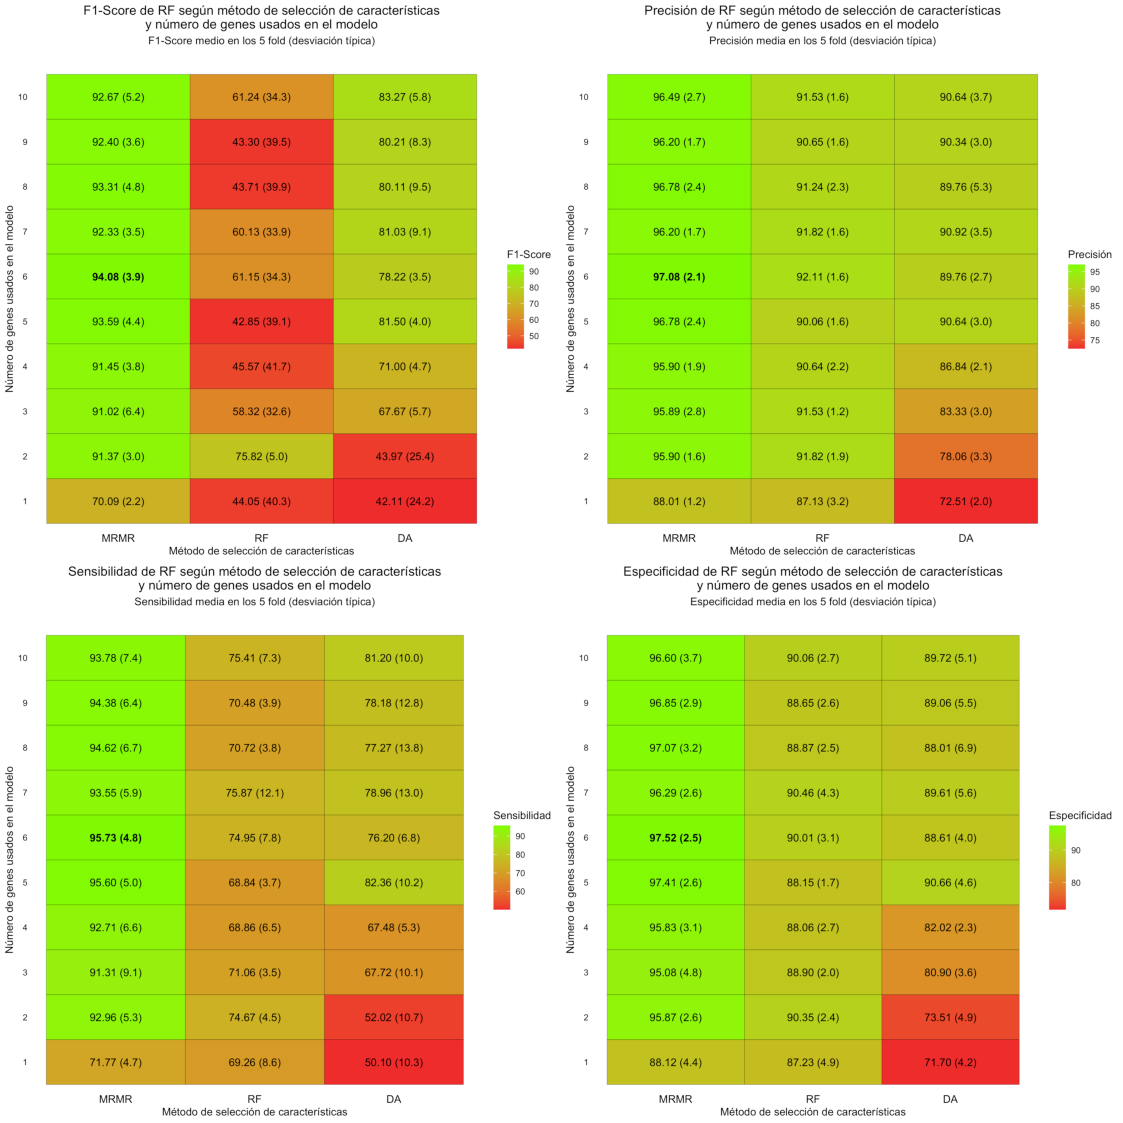
\includegraphics[width=1\textwidth]{figuras/22_higado_multiclase_heatmap_rf.pdf} 
\end{center}

Para random forest, el mejor F1-Score (94,08\%) se obtiene con el método mRMR, considerando 6 genes. Los 6 genes seleccionados son: ANGPTL6, FTLP3, PLXDC1, RAB25, WDR66
y AP2B1. Se analiza su expresión de genes, utilizando para ello un mapa de calor (Figura 23) y diagramas de caja (Figura 24).\\

\newpage
\begin{center}
\textbf{Figura 23}. Mapa de calor de expresión de genes por tipo de muestra (columna izquierda: rojo = carcinoma hepatocelular, naranja = colangiocarcinoma, verde = tejido sano) en los 6 genes más relevantes encontrados en el mejor modelo de RF con mRMR como método de selección de características.
\end{center}
\begin{center}
	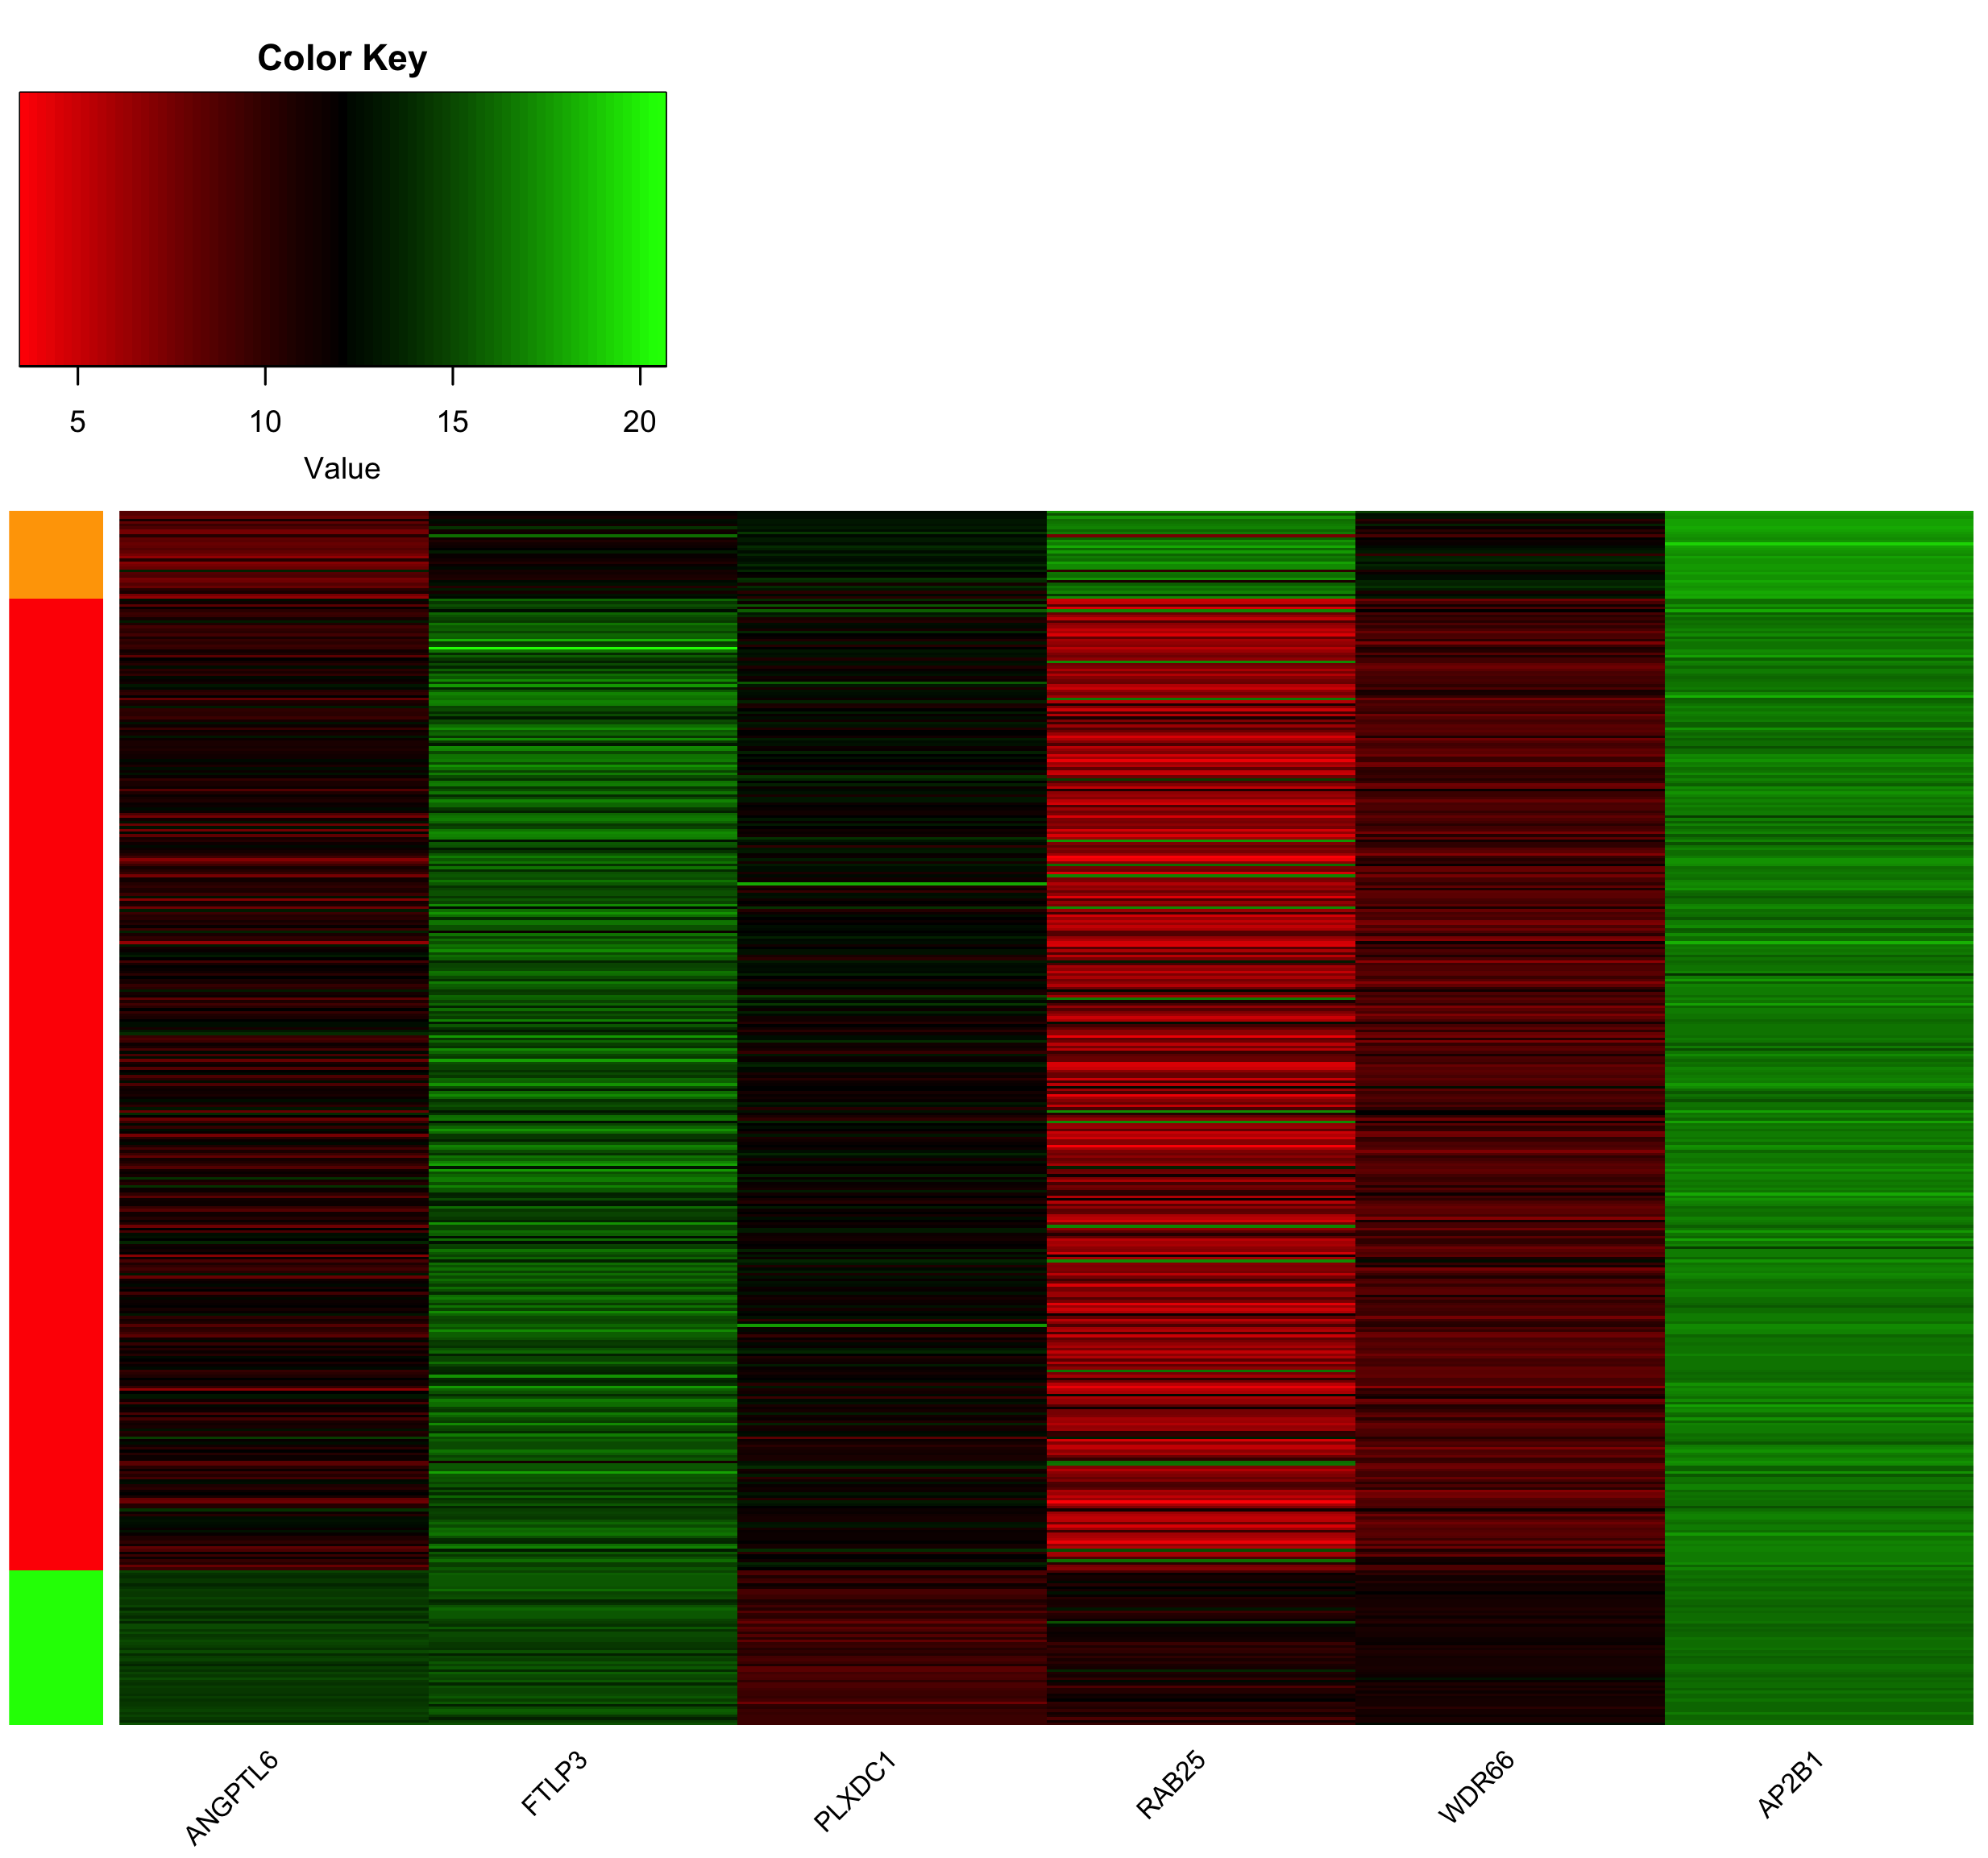
\includegraphics[width=1\textwidth]{figuras/23_higado_multiclase_23_rf_heatmap_mejor_metodo.png} 
\end{center}

\newpage
\begin{center}
\textbf{Figura 24}. Diagrama de caja de expresión de genes por tipo de muestra en los 6 genes más relevantes encontrados en el mejor modelo de RF con mRMR como método de selección de características.
\end{center}
\begin{center}
	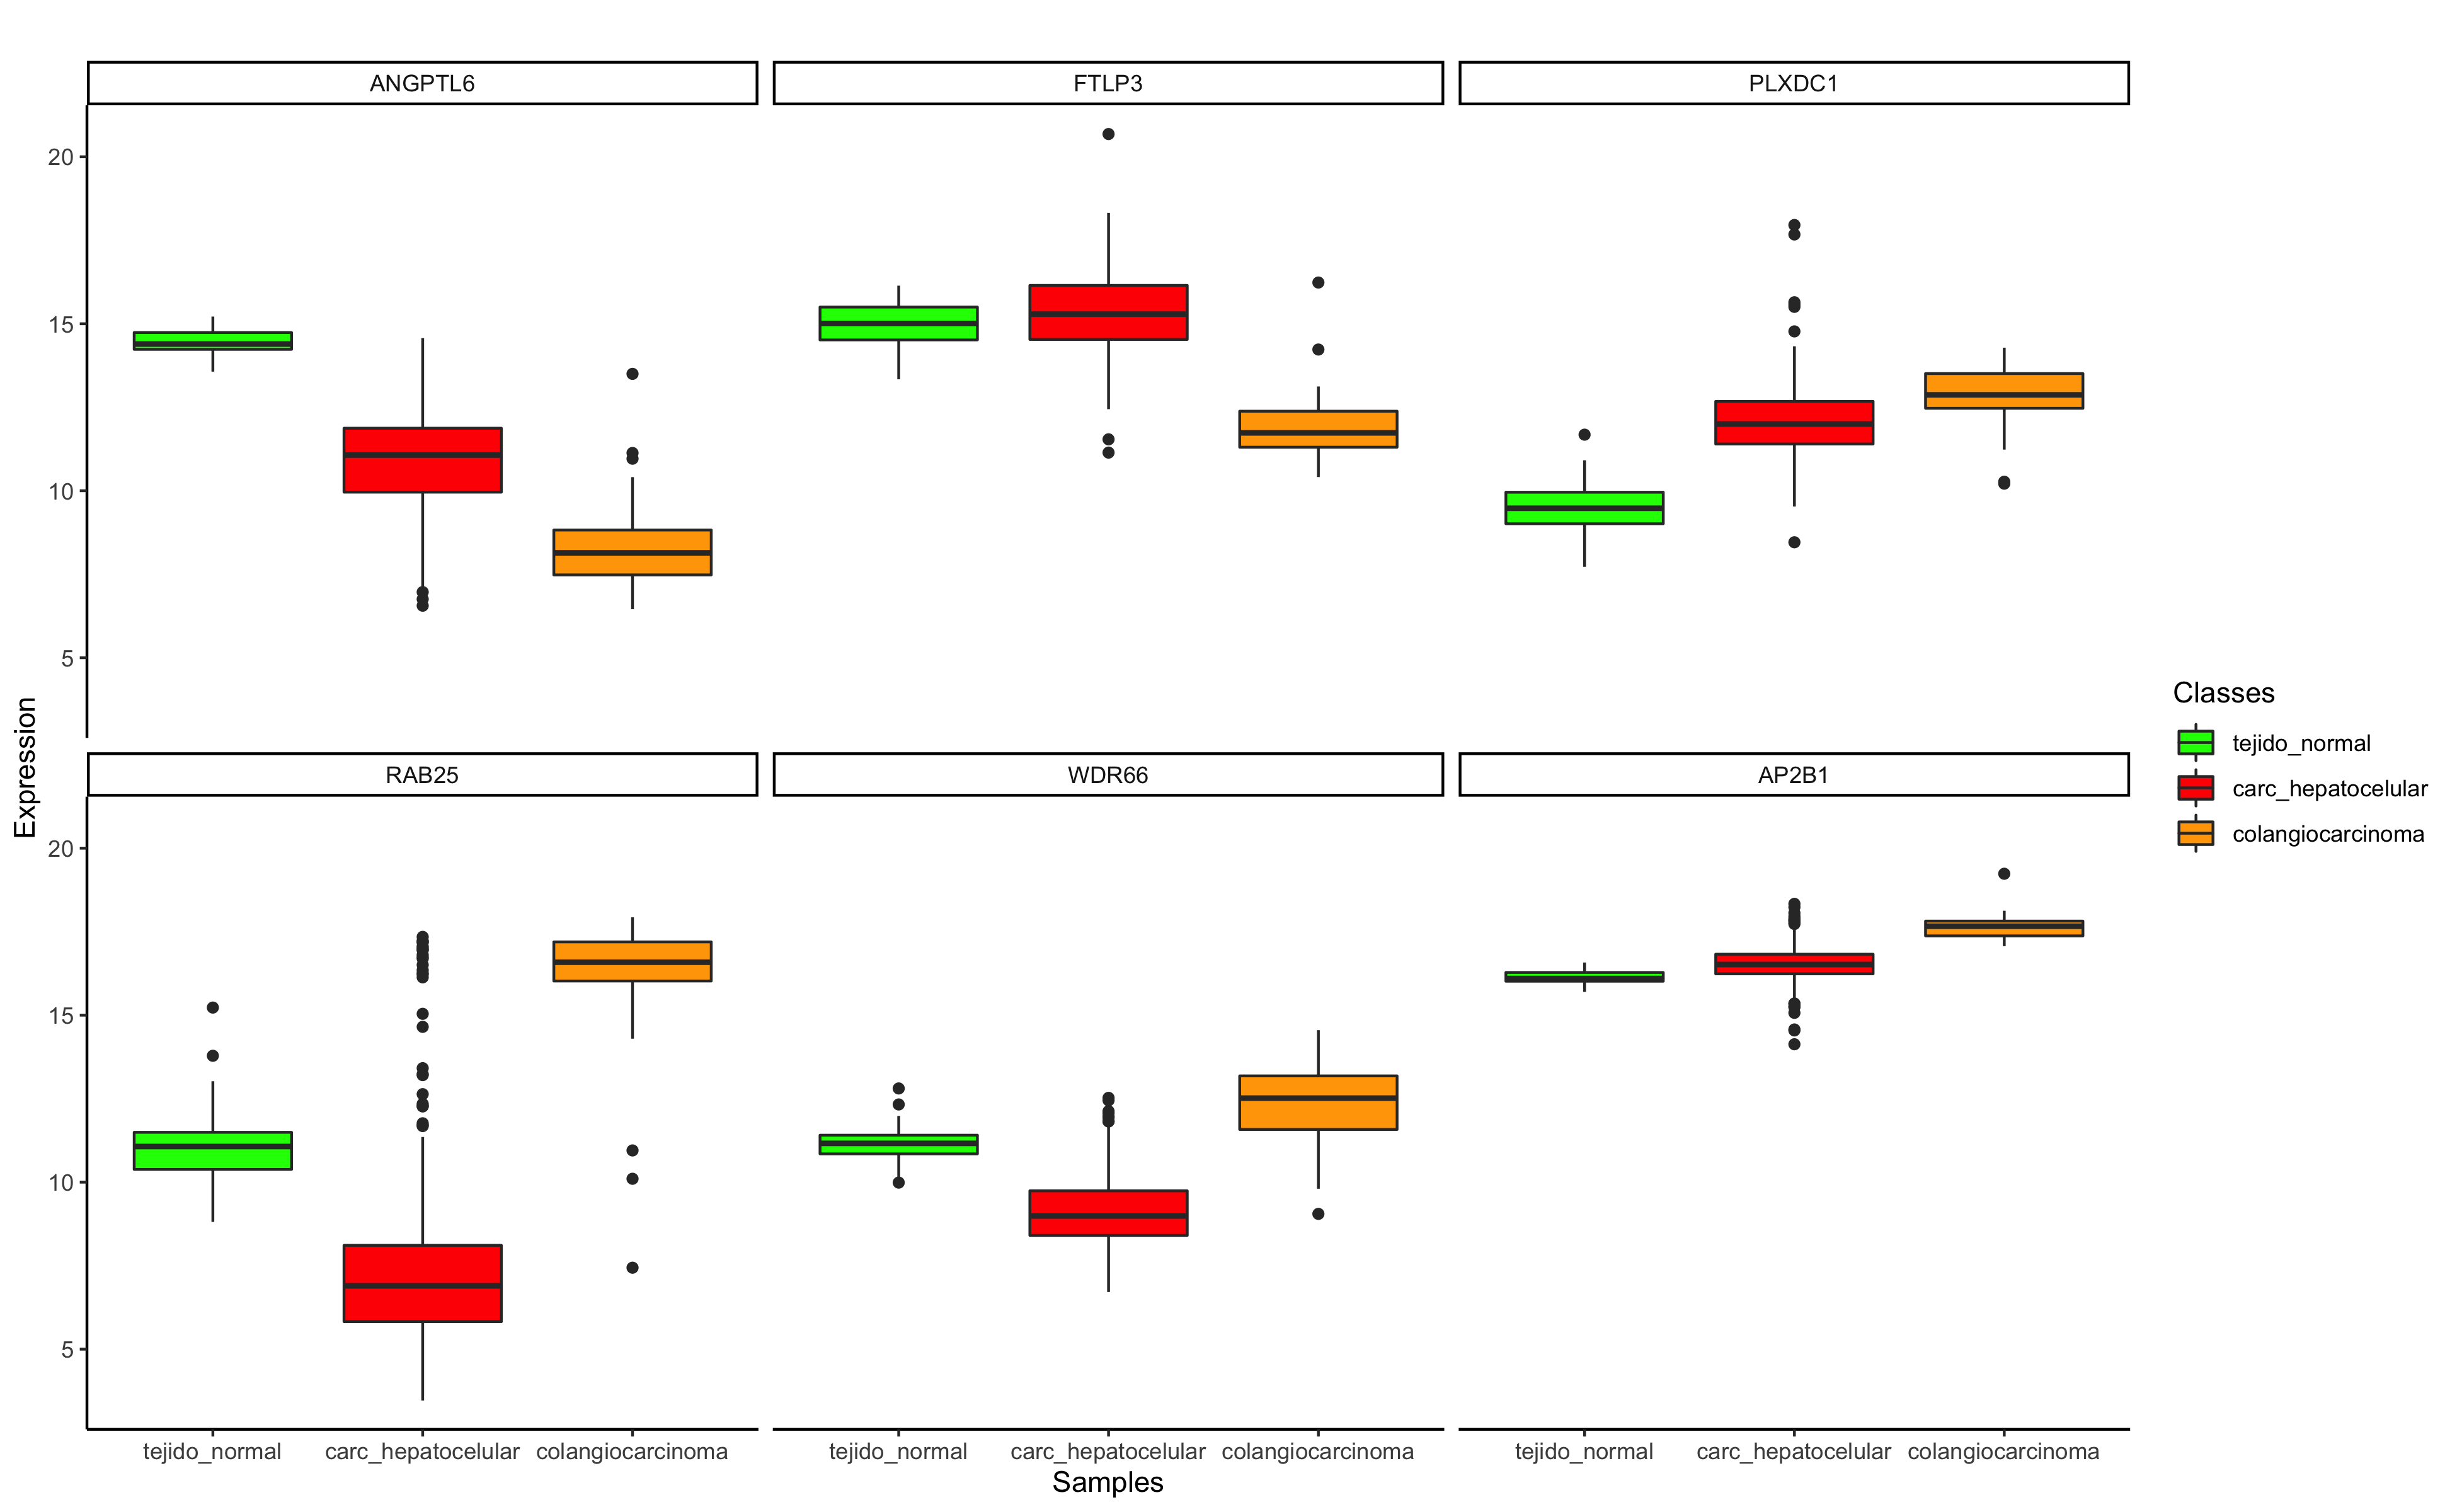
\includegraphics[width=1\textwidth]{figuras/24_higado_multiclase_24_rf_boxplots_mejor_metodo.png} 
\end{center}

\subsection{Validación cruzada en entrenamiento - kNN}

En la Tabla 24 se muestra el número óptimo de vecinos para los 10 genes más relevantes para mRMR, RF y DA.\\

\textbf{Tabla 24}. Número óptimo de vecinos encontrado para los 10 genes más relevantes de cada método de selección de características.

\begin{table}[H]
	\centering
	\begin{tabular}{cccc}
		\cline{2-4}
		\textbf{} & \textbf{mRMR} & \textbf{RF} & \textbf{DA} \\ \hline
		k                &    7 &   9     &   13      \\ \hline
	\end{tabular}
\end{table}

En la Figura 25 se muestran las medidas de evaluación medias obtenidas en las 5 fold.\\

\newpage
\begin{center}
\textbf{Figura 25}. Mapa de calor con valores medios y desviación típica de los 5-fold de F1-Score, precisión, sensibilidad y especificidad de kNN según método de selección de características y número de genes usados.
\end{center}
\begin{center}
	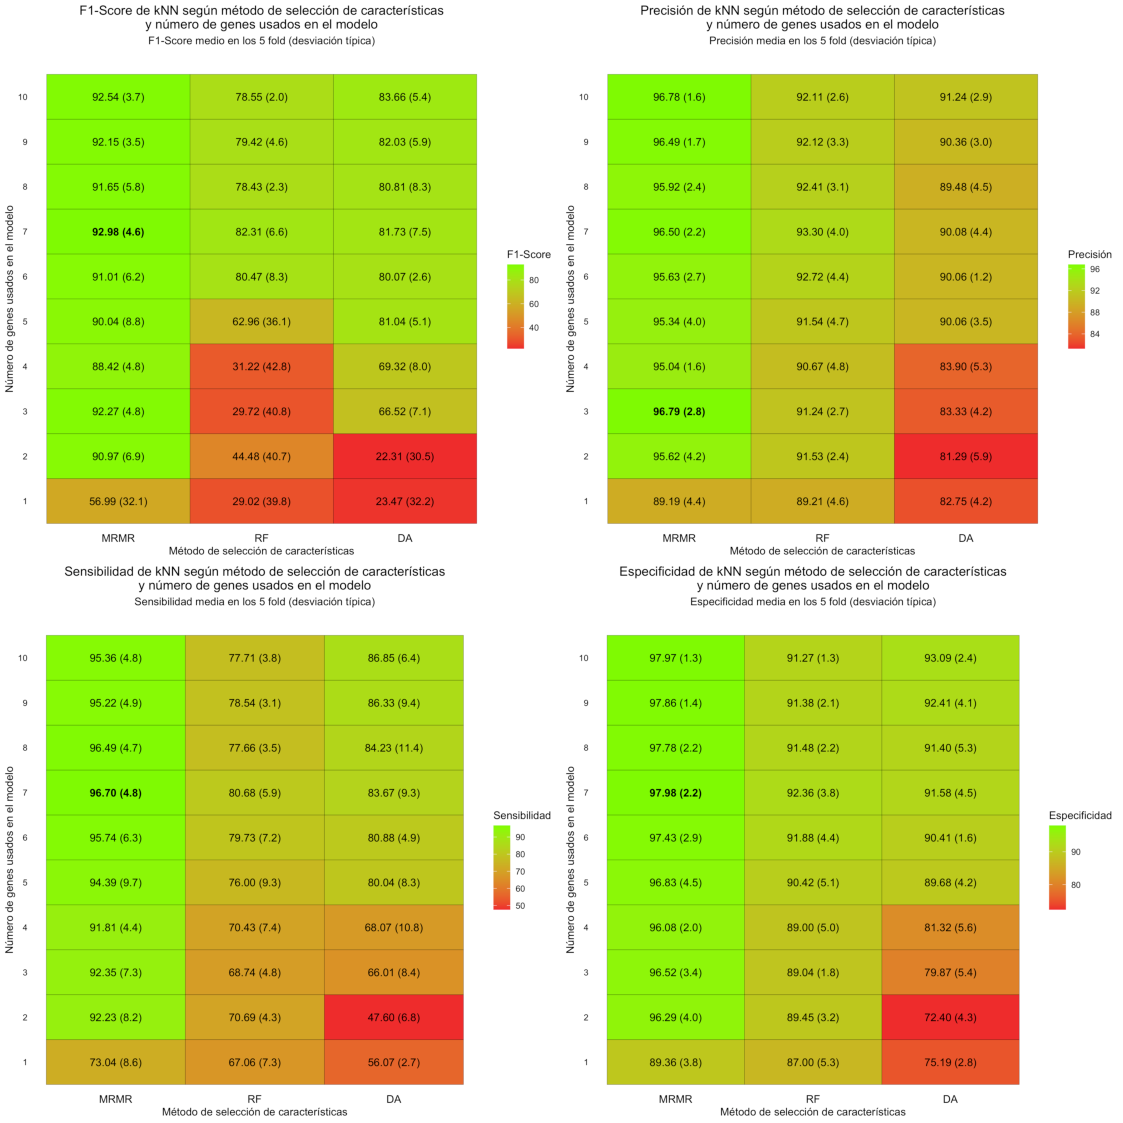
\includegraphics[width=1\textwidth]{figuras/25_higado_multiclase_heatmap_knn.pdf} 
\end{center}

Para kNN, el mejor F1-Score (92,98\%) se obtiene con el método mRMR para 7 genes. Los 7 genes seleccionados son: ANGPTL6, FTLP3, PLXDC1, RAB25, WDR66, AP2B1 y CDH13. Se analiza su expresión de genes, utilizando para ello un mapa de calor (Figura 26) y diagramas de caja (Figura 27).

\newpage
\begin{center}
\textbf{Figura 26}. Mapa de calor de expresión de genes por tipo de muestra (columna izquierda: rojo = carcinoma hepatocelular, naranja = colangiocarcinoma, verde = tejido sano) en los 7 genes más relevantes encontrados en el mejor modelo de kNN con mRMR como método de selección de características.
\end{center}
\begin{center}
	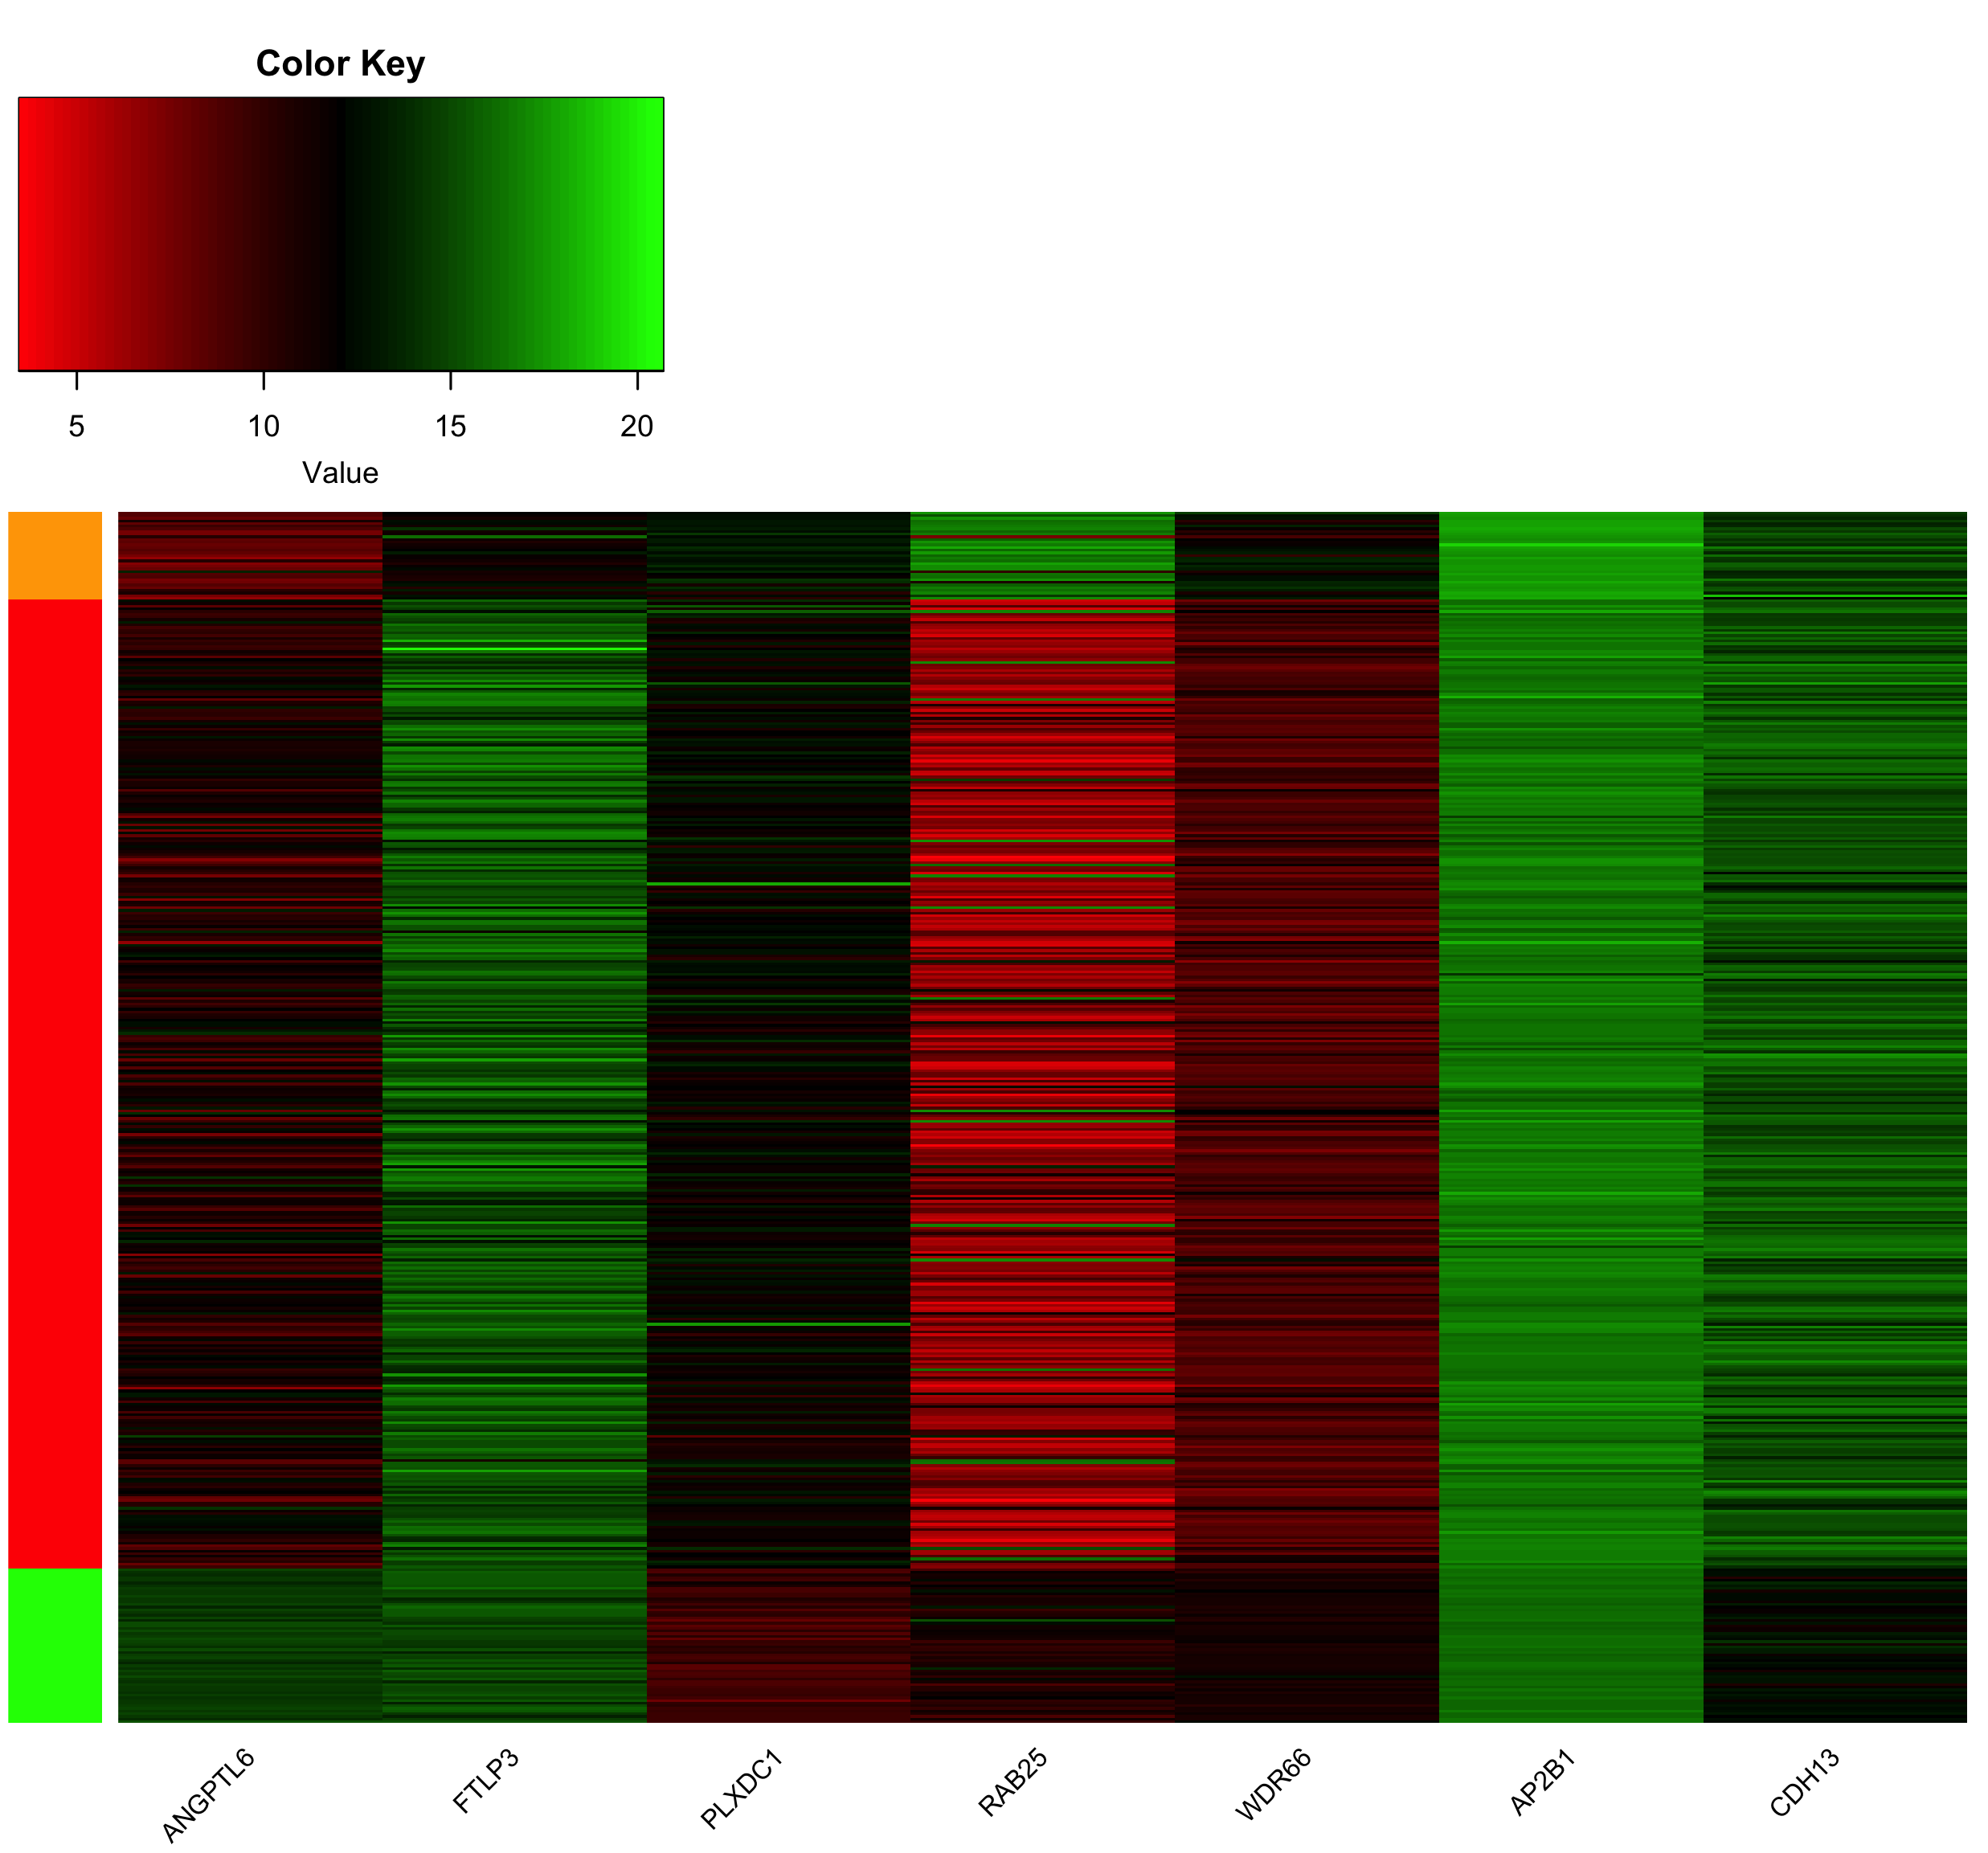
\includegraphics[width=1\textwidth]{figuras/26_higado_multiclase_33_knn_heatmap_mejor_metodo.png} 
\end{center}

\newpage
\begin{center}
\textbf{Figura 27}. Diagrama de caja de expresión de genes por tipo de muestra en los 7 genes más relevantes encontrados en el mejor modelo de kNN con mRMR como método de selección de características.
\end{center}
\begin{center}
	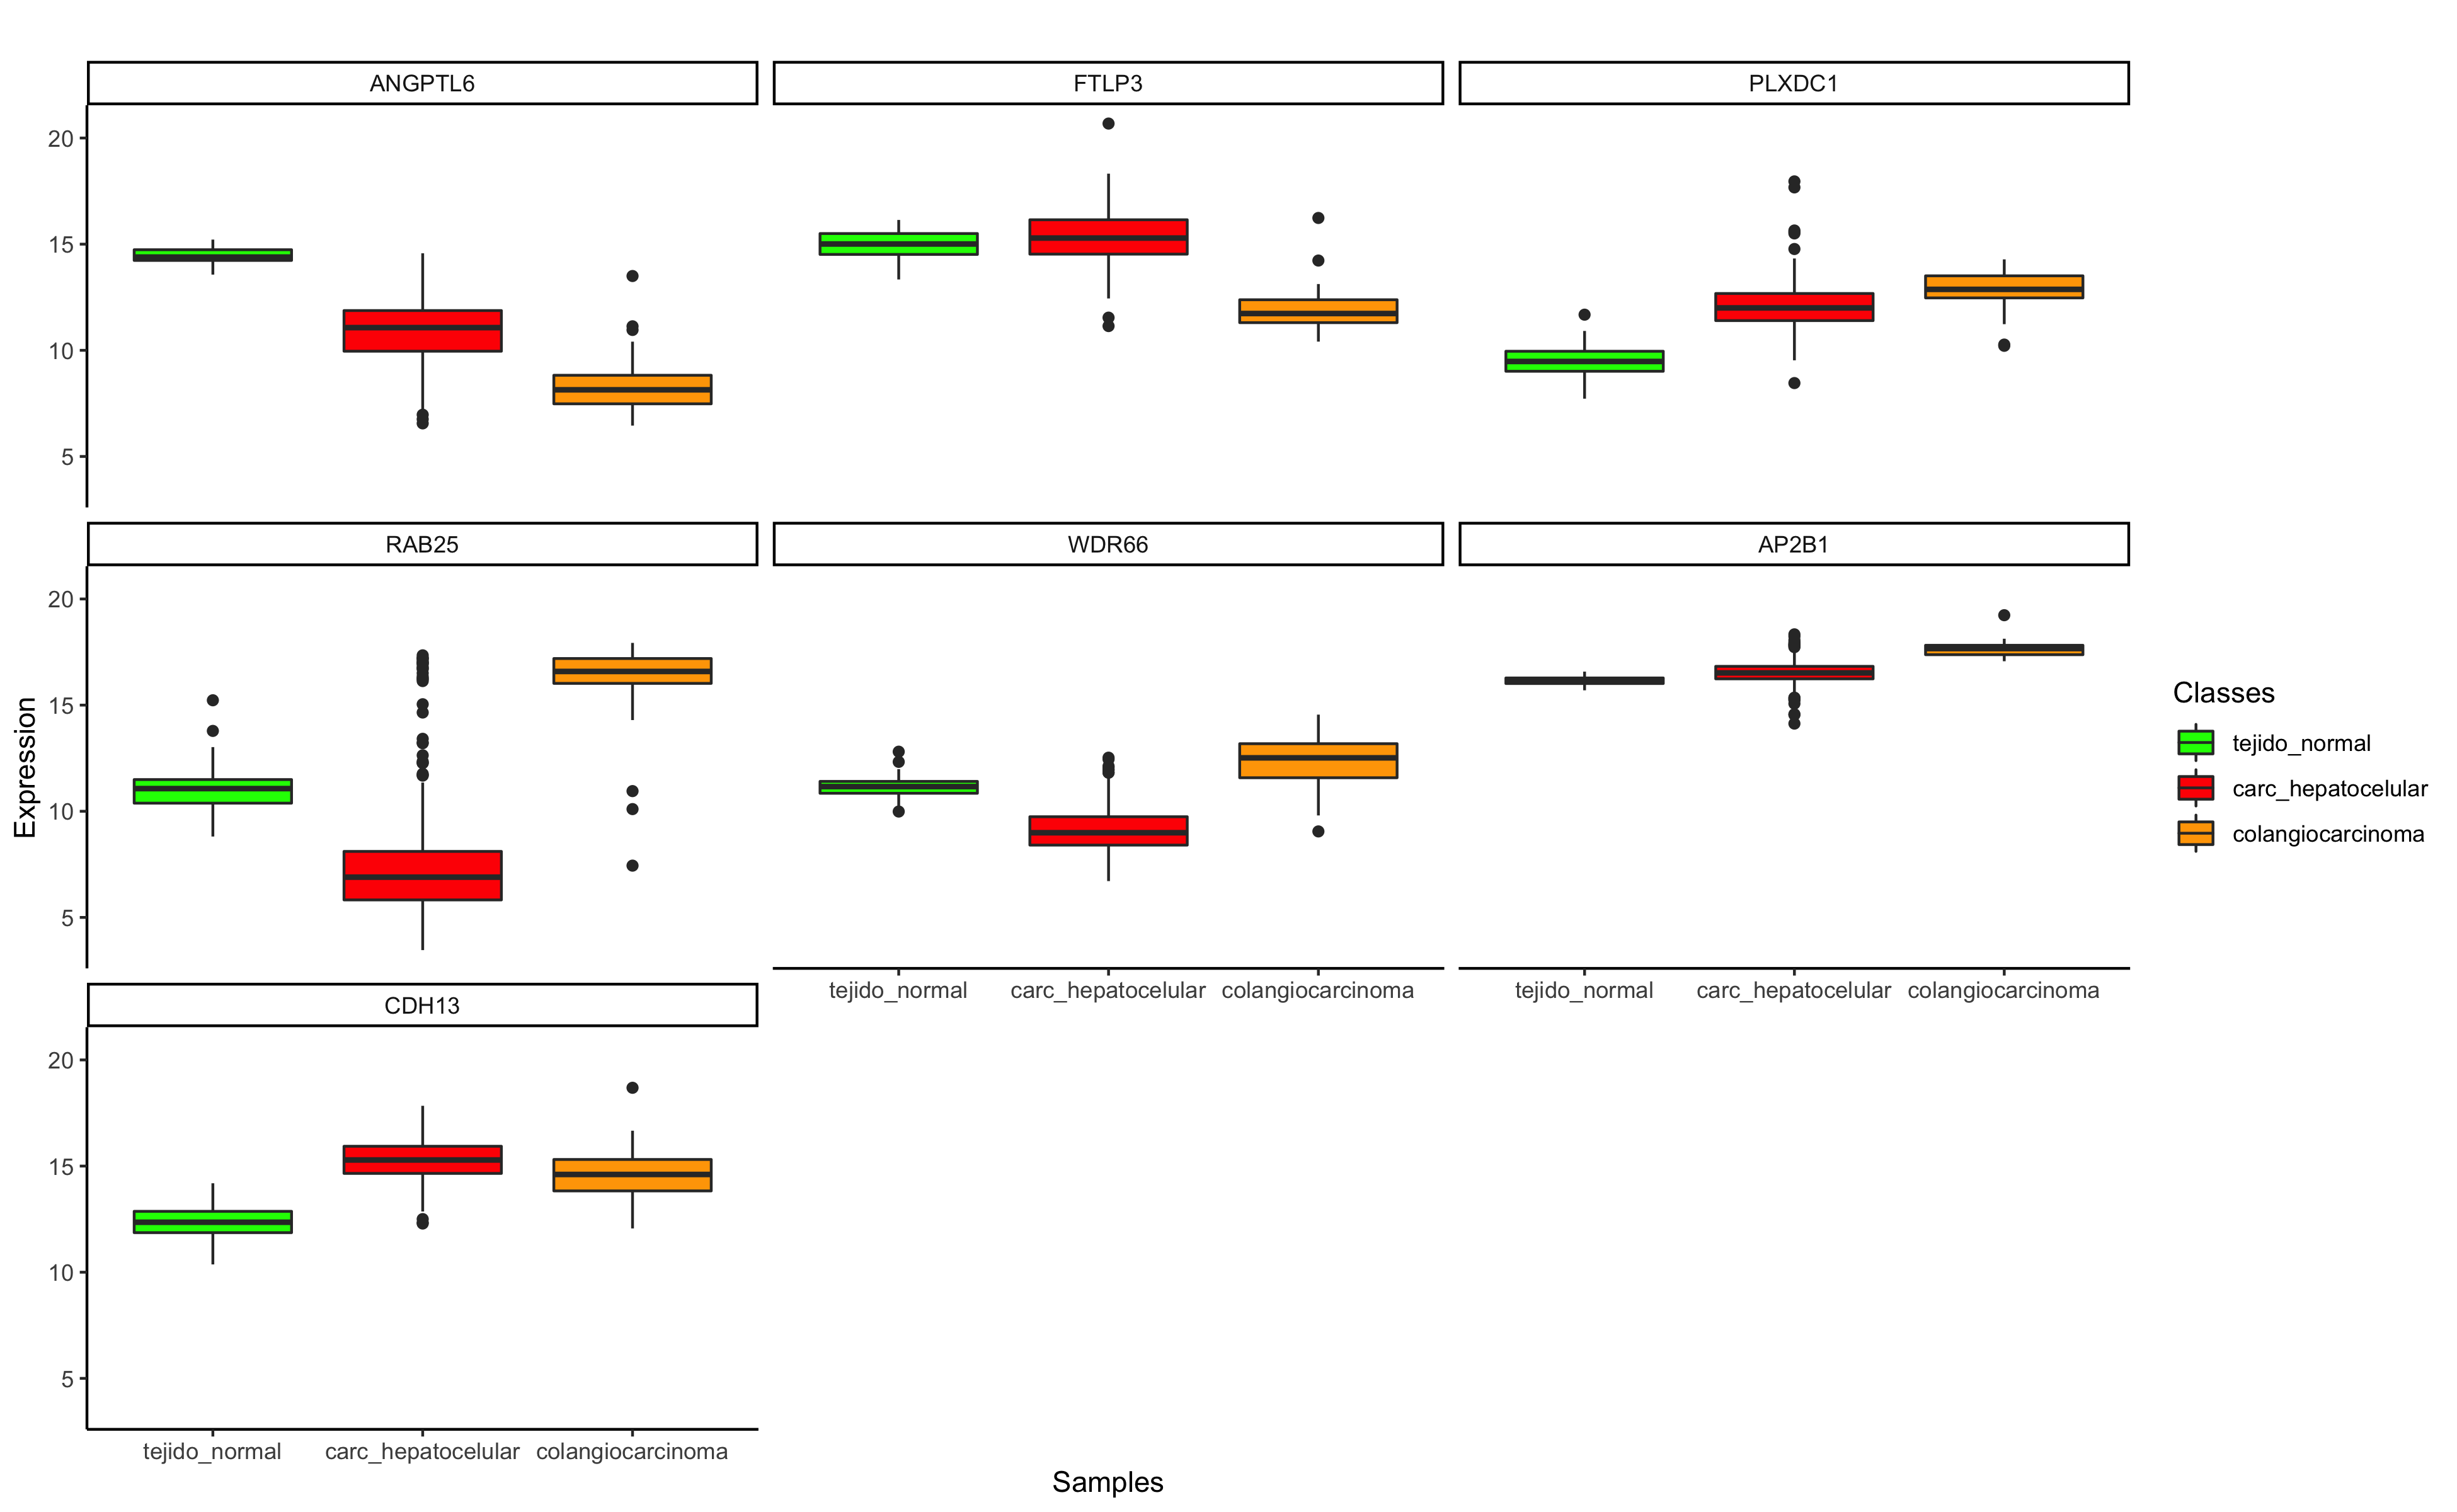
\includegraphics[width=1\textwidth]{figuras/27_higado_multiclase_34_knn_boxplots_mejor_metodo.png} 
\end{center}

\subsection{Validación en test}

Al validar en el conjunto de test el mejor modelo encontrado para SVM y kNN (ambas con 7 genes con mRMR),  se obtiene la misma clasificación, descrita en la Figura 28, con F1-Score en test es de 91,8\% y una precisión de 96,4\%.\\

\newpage
\begin{center}
\textbf{Figura 28}. Matriz de confusión de los mejores modelos encontrados de SVM y kNN en el conjunto de test.
\end{center}

\begin{center}
	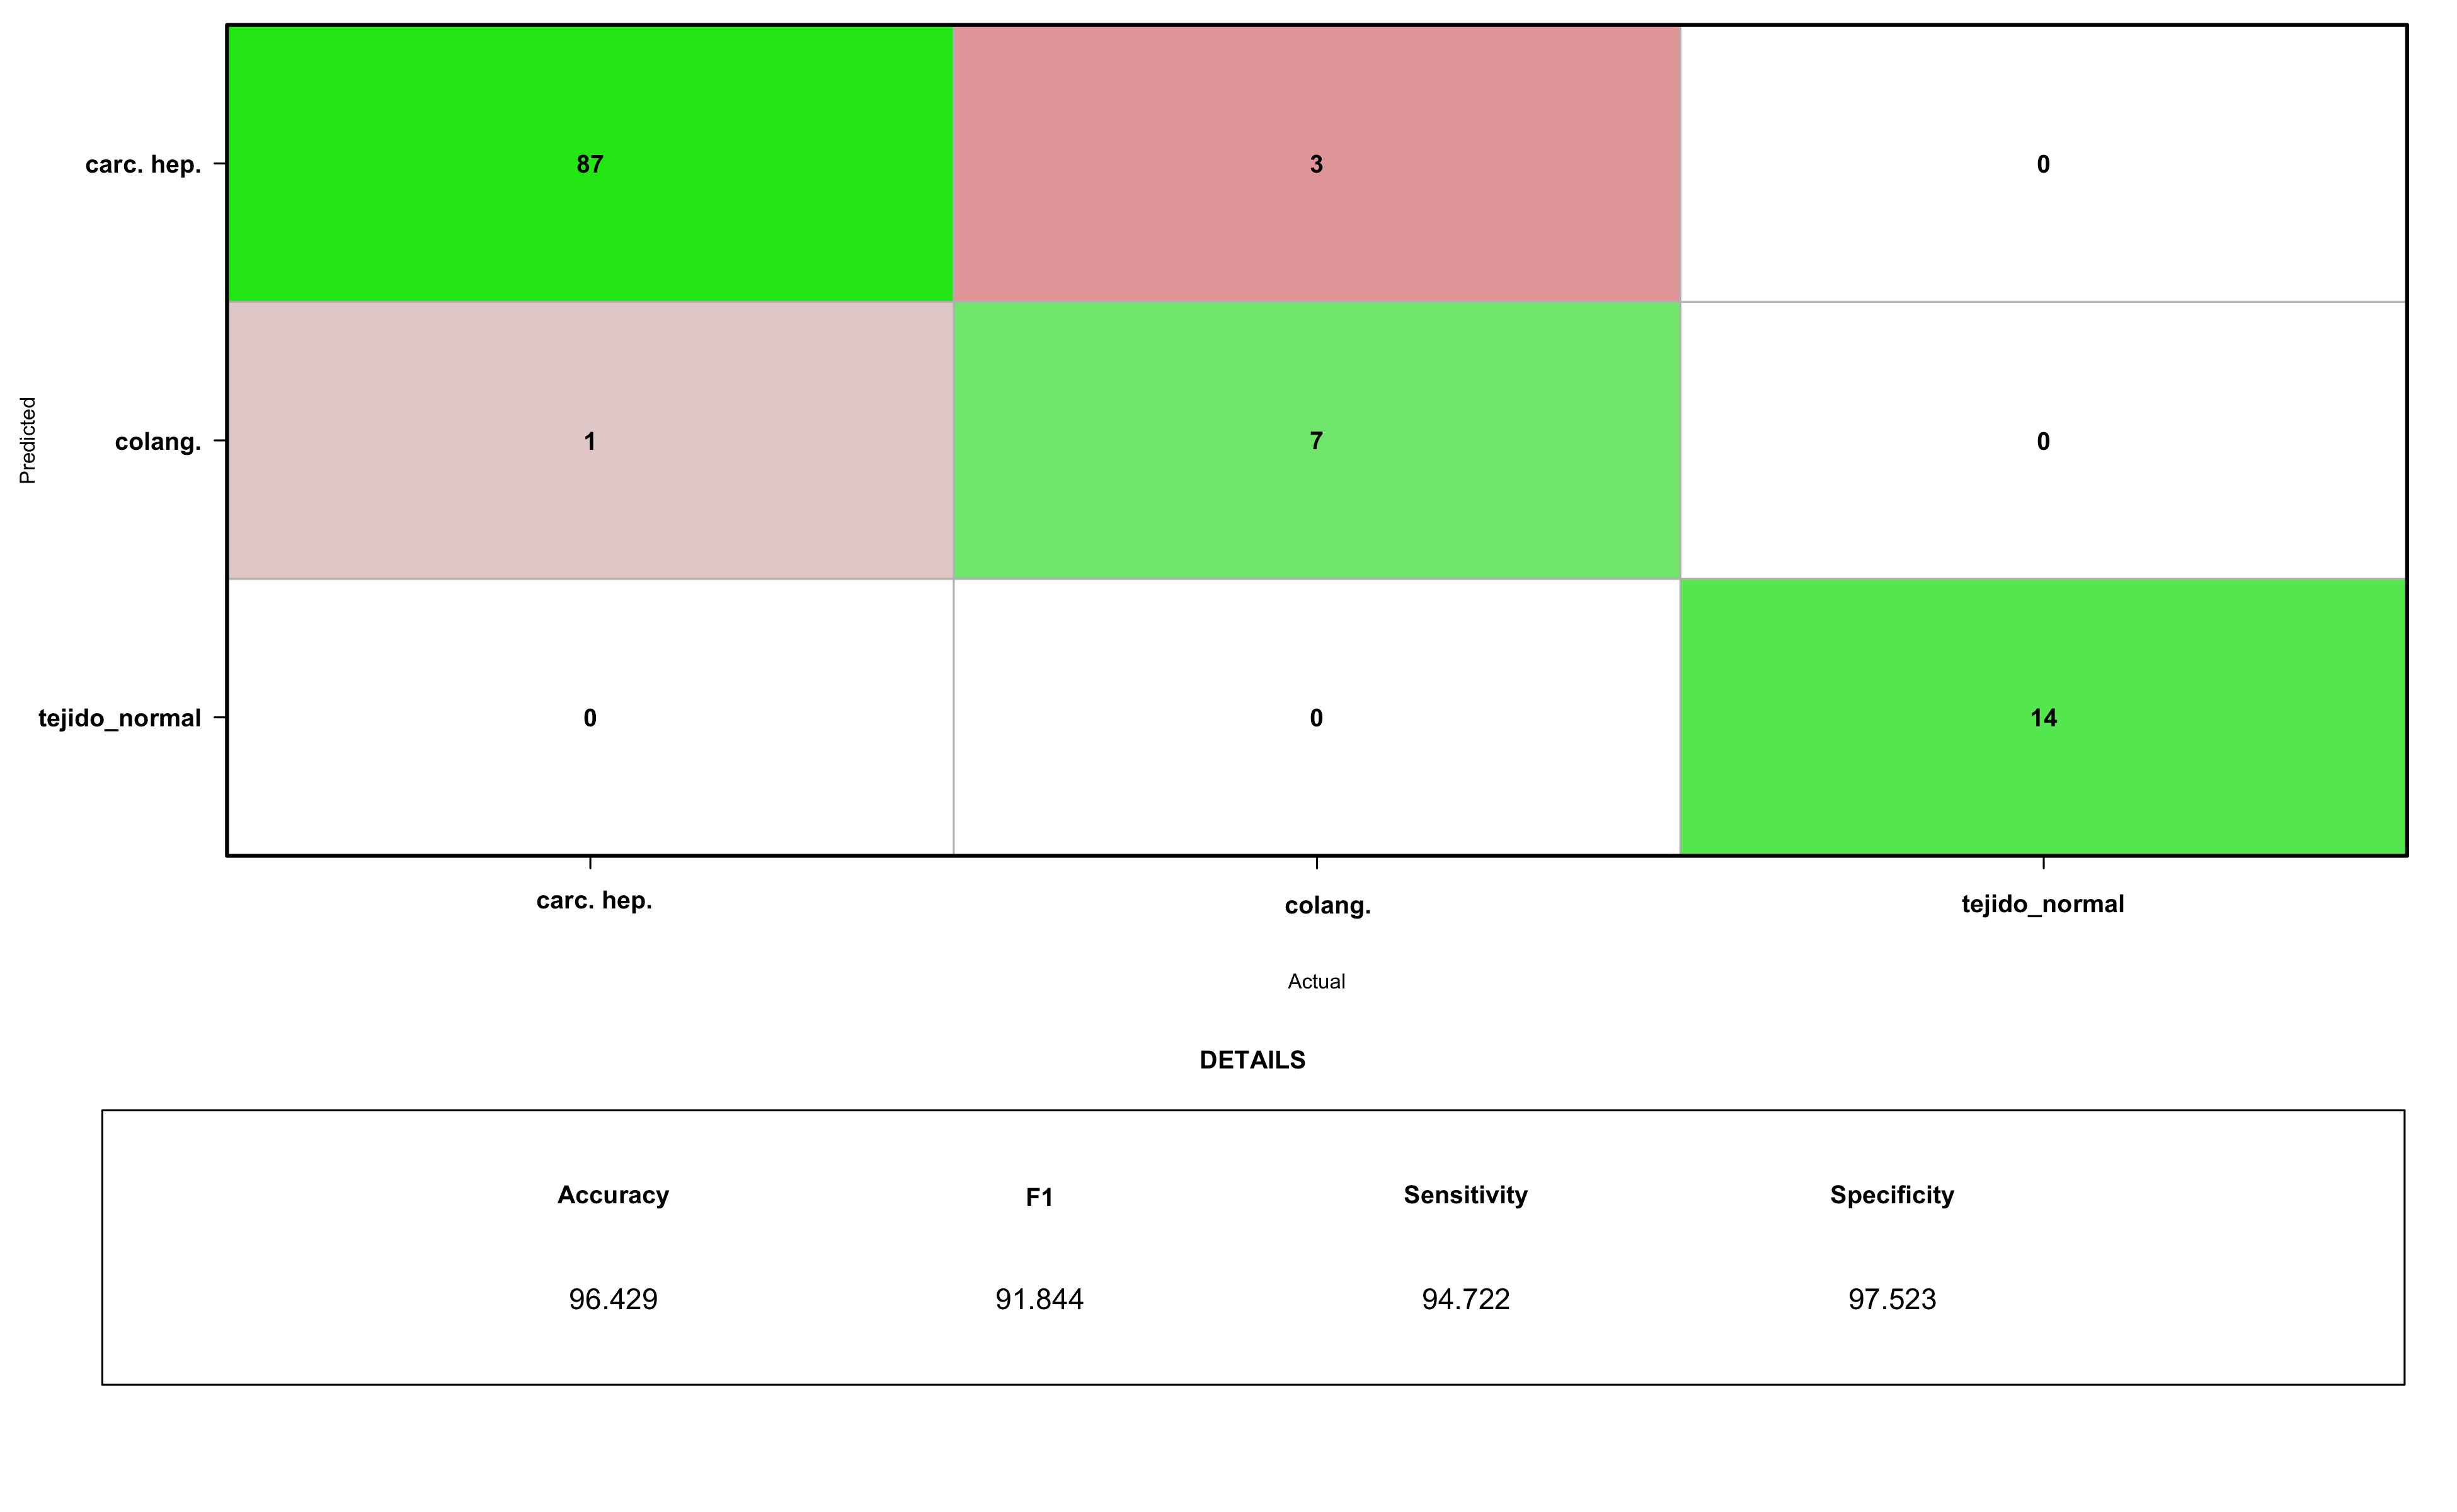
\includegraphics[width=1\textwidth]{figuras/28_higado_multiclase_15_svm_matriz_confusion_mejor_metodo_mejorado.png} 
\end{center}

La validación en el conjunto de test del mejor modelo encontrado para RF (6 genes con mRMR) se muestra en la Figura 29, siendo los resultados ligeramente inferiores a los obtenidos con SVM y kNN.\\

\newpage
\begin{center}
\textbf{Figura 29}. Matriz de confusión del mejor modelo encontrado de RF en el conjunto de test.
\end{center}
\begin{center}
	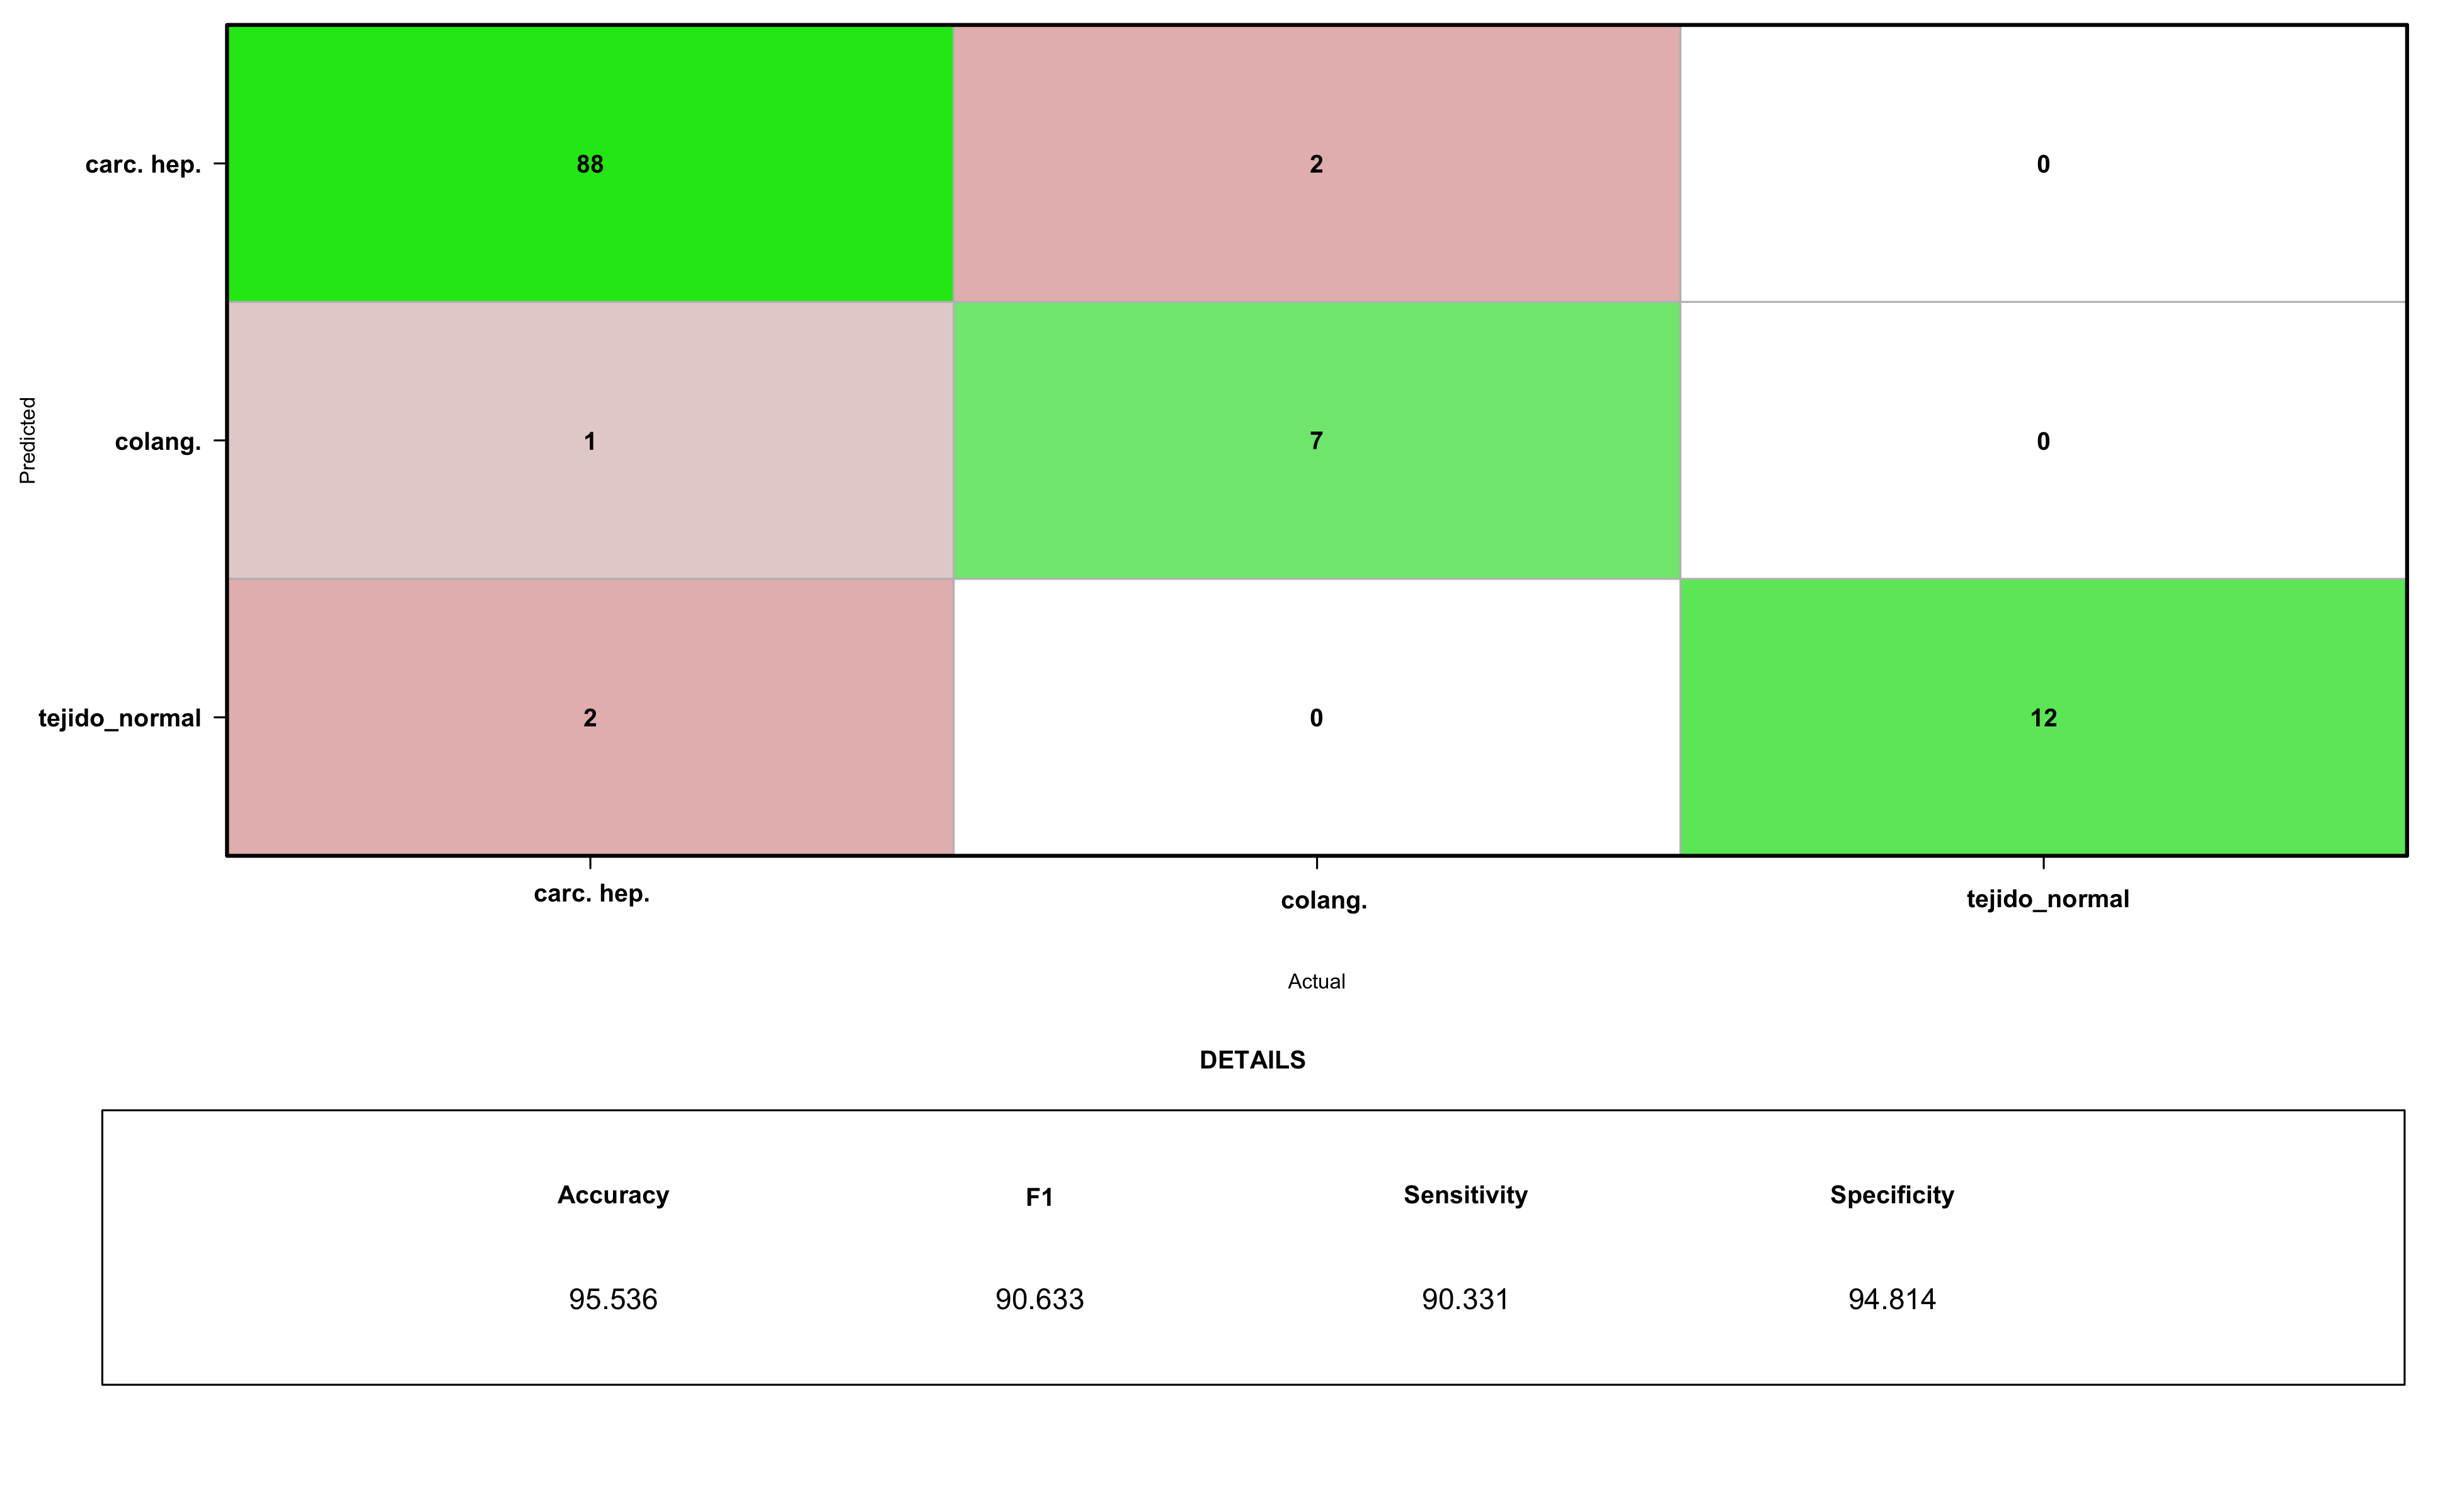
\includegraphics[width=1\textwidth]{figuras/29_higado_multiclase_25_rf_matriz_confusion_mejor_metodo_mejorado.png} 
\end{center}

En la Tabla 25 se muestra un resumen de los mejores modelos obtenidos y su F1-Score y precisión en conjunto de entrenamiento y conjunto de test.\\

\textbf{Tabla 25}. Resumen de clasificación multiclase para cáncer de hígado. Mejor modelo encontrado para SVM, RF y kNN con biomarcadores seleccionados, parámetros optimizados para cada algoritmo, F1-Score y precisión (Acc) en conjunto de entrenamiento y conjunto de test.

\begin{table}[H]
	\centering
	\begin{tabular}{ccccc|cc}
		\cline{2-7}
		& Biomarcadores & Parámetros                                                         & F1 train & Acc train & F1 test & Acc test \\ \hline
		SVM &  \textbf{7 genes} mRMR  & \begin{tabular}[c]{@{}c@{}}$c$ = 1\\ $\gamma$ = 0.025\end{tabular} & 94,99    & 97,66     & 91,84   & 96,43    \\ \hline
		RF  &  \textbf{6 genes} mRMR & --                                                                 & 94,08    & 97,08     & 90,63   & 95,54    \\ \hline
		kNN &  \textbf{7 genes} mRMR & k = 7                                                              & 92,98    & 96,79     & 91,84   & 96,43    \\ \hline
	\end{tabular}
\end{table}

\subsection{Conclusiones}

Como conclusión, los mejores modelos de SVM y kNN distinguen bien entre tejido tumoral y tejido sano, pero cometen 4 errores distinguiendo carcinomas hepatocelulares de colangiocarcinomas. Estos errores cometidos en la clasificación pueden ser debidos a similitudes biológicas entre ambos tipos de cáncer. El mejor modelo de RF distingue ligeramente mejor entre los dos tipos de cáncer, aunque predice como tejido normal dos casos de carcinoma hepatocelular.\\

En la plataforma de Open Targets \cite{OpenTargets2020} se encuentra asociación entre todos los genes de los mejores modelos (7 mejores genes de mRMR) y el cáncer excepto para FTLP3, que es un pseudogen (gen que ha perdido su funcionalidad) \cite{Guo2014}. El gen CDH13 tiene además relación directa con el cáncer de hígado. Por otra parte, algunos genes están relacionados con factores de riesgo del cáncer de hígado: PLXDC1 y AP2B1 con hábito tabáquico \cite{Liu2019} y CDH13 con consumo de alcohol \cite{Schumann2016}.

\section{Resultados de clasificación biclase para cáncer de colon-recto}

El código completo del análisis se muestra en el fichero \textit{\texttt{analisis\_cr/\linebreak03\_analisis\_biclase.R}} del repositorio de GitHub asociado al trabajo \cite{Redondo-Sanchez2020}.

\subsection{Detección de biomarcadores}

Para la clasificación biclase en cáncer de colon-recto se cuenta con 644 tumores y 51 muestras de tejido sano (Tabla 26).\\

\textbf{Tabla 26}. Distribución de tipos de muestra para el análisis de cáncer de colon-recto biclase.

\begin{table}[H]
	\centering
	\begin{tabular}{lcc}
		\cline{2-3}
		& \textbf{Número de casos} & \textbf{Porcentaje} \\ \hline
		\textbf{Tumor}     & 644        & 92,7\%              \\
		\textbf{Tejido sano} & 51         & 7,3\%              \\ \hline
		\textbf{Total}       & 695        & 100\%               \\ \hline
	\end{tabular}
\end{table}

Se extraen 6.836 genes que presentan en su expresión diferencias significativas entre las muestras de tumor y las de tejido sano. En la Tabla 27 se muestra la partición entrenamiento - test realizada y en la figura 30 se representa en un diagrama de Sankey.

\newpage
\textbf{Tabla 27}. Distribución entrenamiento-test según tipo de muestra y proporción entre clases para el análisis de colon-recto biclase.

\begin{table}[H]
	\centering
	\begin{tabular}{lccc}
		\cline{2-4}
		\multicolumn{1}{c}{\textbf{}}                                               & \textbf{Total} & \textbf{Entrenamiento} & \textbf{Test} \\ \hline
		\textbf{Tumores}                                                            & 644 (100\%)    & 483 (75,0\%)           & 161 (25,0\%)  \\
		\textbf{Tejido sano}                                                        & 51 (100\%)     & 39 (76,5\%)            & 12 (23,5\%)   \\ \hline
		\textbf{\begin{tabular}[c]{@{}l@{}}Proporción\\ tumores/sanos\end{tabular}} & 12,6           & 12,4                   & 13,4          \\ \hline
	\end{tabular}
\end{table}

\begin{center}
\textbf{Figura 30}. Diagrama de Sankey mostrando la partición entrenamiento-test realizada según tipo de muestra para el análisis de colon-recto biclase.
\end{center}
\begin{center}
	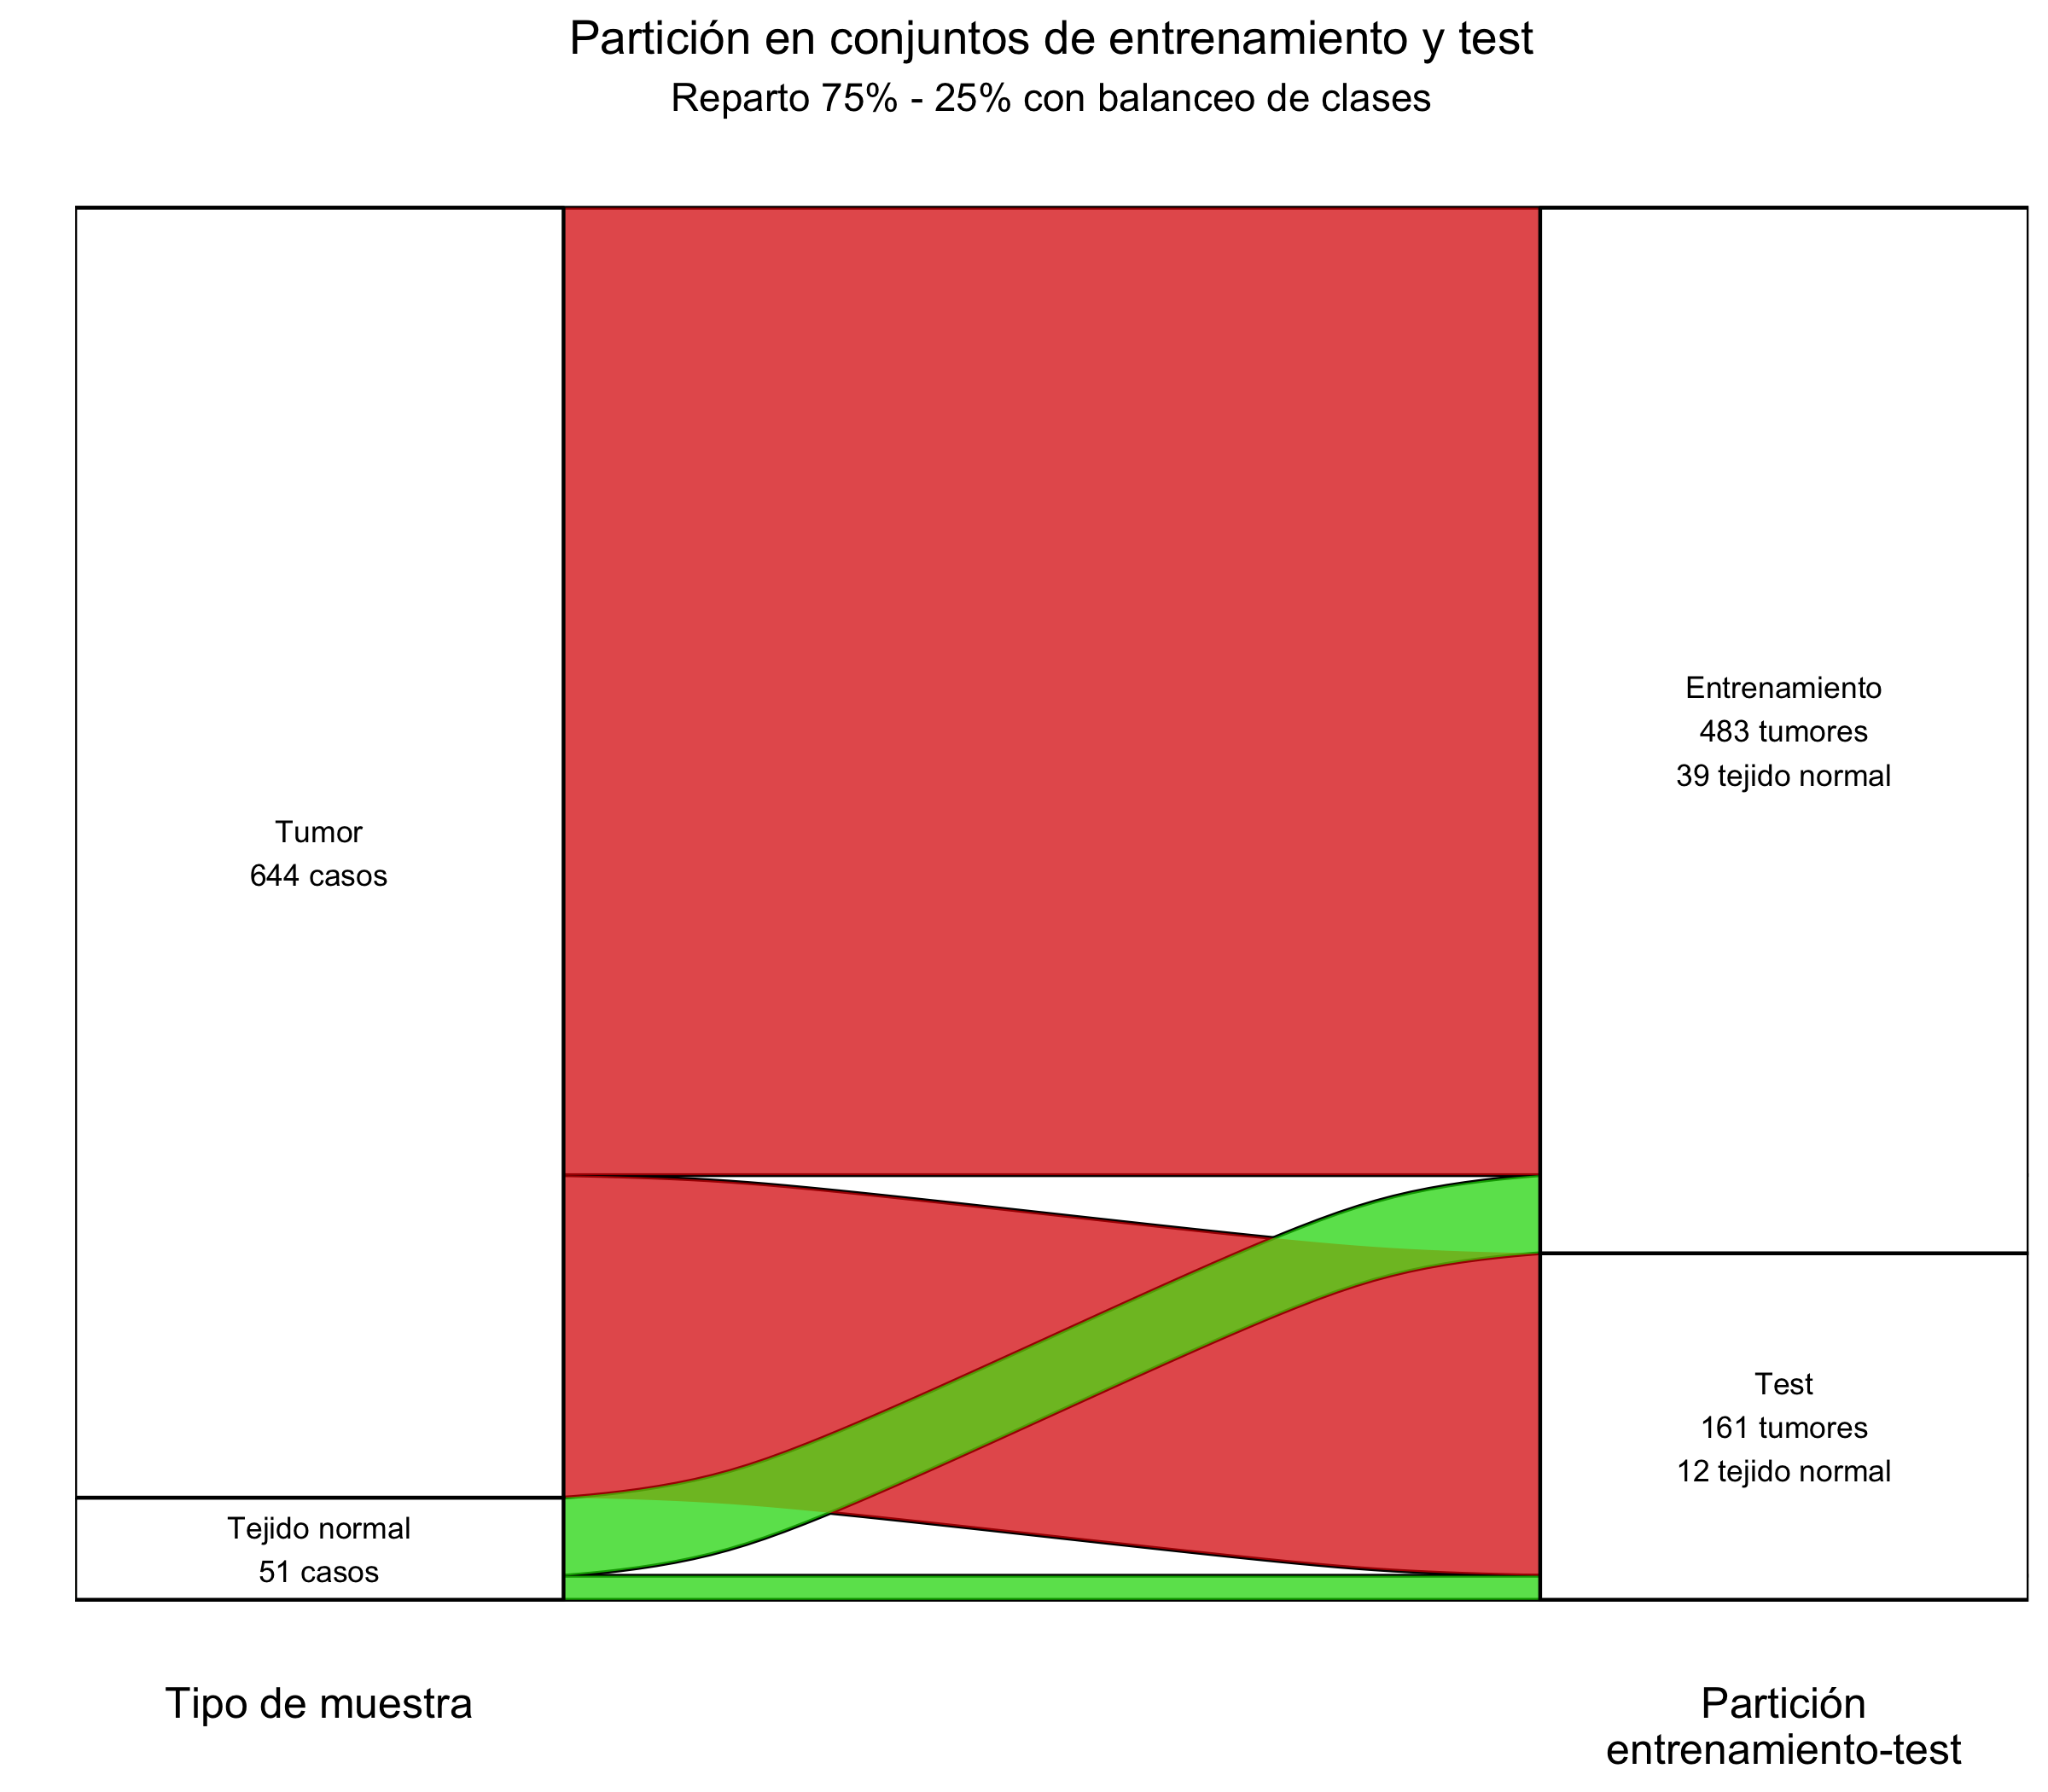
\includegraphics[width=.75\textwidth]{figuras/30_cr_biclase_05_sankey.png}
\end{center}

\newpage
A continuación se muestran los diez genes más relevantes encontrados por cada método de selección de características:\\

\textbf{Tabla 28}. Diez genes más relevantes según los distintos métodos de selección de características para el análisis de colon-recto biclase.

\begin{table}[H]
	\centering
	\begin{tabular}{clll}
		\hline
		\textbf{Ranking} & \multicolumn{1}{c}{\textbf{mRMR}} & \multicolumn{1}{c}{\textbf{RF}} & \multicolumn{1}{c}{\textbf{DA}} \\ \hline
		1                & BEST4                             & VSTM2A                          & ETV4                            \\
		2                & MET                               & CA7                             & SCN7A                           \\
		3                & EPOP                              & COL11A1                         & RSPO2                           \\
		4                & RXRG                              & GLP2R                           & PHOX2B                          \\
		5                & C5orf34                           & SLC39A10                        & SALL4                           \\
		6                & DHRS7C                            & ENC1                            & POU5F1B                         \\
		7                & NKX2-3                            & ESM1                            & TNFRSF17                        \\
		8                & ESM1                              & CEMIP                           & SCN9A                           \\
		9                & SGCG                              & CA2                             & TLX1                            \\
		10               & MDFI                              & KRT80                           & WT1                             \\ \hline
	\end{tabular}
\end{table}

Se observa que el gen ESM1 es el único gen común a dos algoritmos de selección de características: mRMR y RF.

\subsection{Validación cruzada en entrenamiento}

En las Tablas 29 y 30 se muestran los parámetros óptimos de SVM y kNN obtenidos.\\

\textbf{Tabla 29}. Parámetros óptimos de SVM encontrados para los 10 genes más relevantes de cada método de selección de características.

\begin{table}[H]
	\centering
	\begin{tabular}{cccc}
		\hline
		\textbf{Parámetro} & \textbf{mRMR} & \textbf{RF} & \textbf{DA} \\ \hline
		Coste                &    0,05 &    0,05     &  0,05       \\
		Gamma               &     0,06    &     0,07   & 0,06        \\ \hline
	\end{tabular}
\end{table}

\textbf{Tabla 30}. Número óptimo de vecinos encontrado para los 10 genes más relevantes de cada método de selección de características.

\begin{table}[H]
	\centering
	\begin{tabular}{cccc}
		\cline{2-4}
		\textbf{} & \textbf{mRMR} & \textbf{RF} & \textbf{DA} \\ \hline
		k                &   23 &   23     &   23      \\ \hline
	\end{tabular}
\end{table}

En la Figura 31 se muestran para SVM, RF y kNN el F1-Score medio obtenido en las 5 fold.

\begin{center}
\textbf{Figura 31}. Mapa de calor con valores medios y desviación típica de los 5-fold de F1-Score de SVM, RF y kNN según método de selección de características y número de genes usados.
\end{center}
\begin{center}
	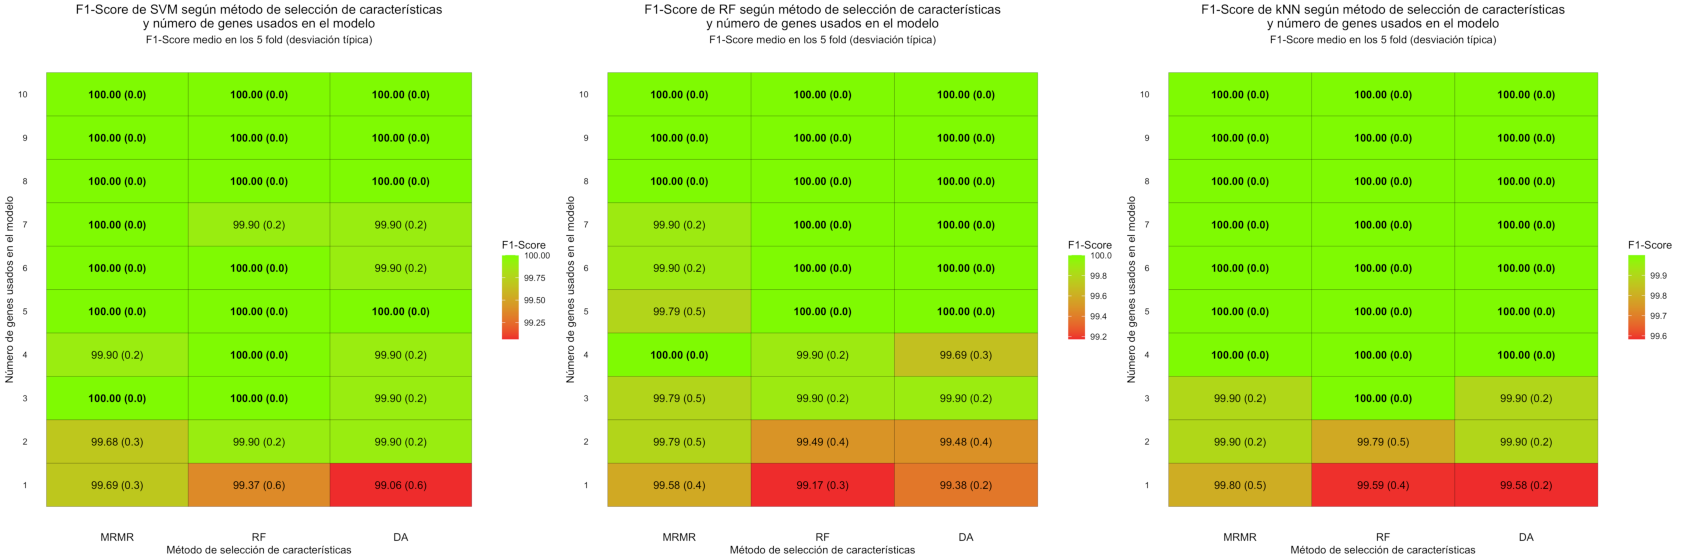
\includegraphics[width=1\textwidth]{figuras/31_cr_biclase_heatmap_horizontal.pdf} 
\end{center}

Se alcanzan F1-Score de 100\% en muchos casos. En caso de igualdad de F1-Score, se seleccionará como mejor modelo aquel que emplee el menor número de genes. Por tanto, los mejores modelos son:
\begin{itemize}
	\item Para SVM: mRMR ó RF con 3 genes.
	\item Para RF: mRMR con 4 genes.
	\item Para kNN: RF con 3 genes.
\end{itemize}

Se analiza la expresión de 3 genes más relevantes de RF y los 4 más relevantes de mRMR con diagramas de caja (Figuras 32 y 33).

\begin{center}
\textbf{Figura 32}. Diagrama de caja de expresión de genes por tipo de muestra en los 3 genes más relevantes con RF como método de selección de características.
\end{center}
\begin{center}
	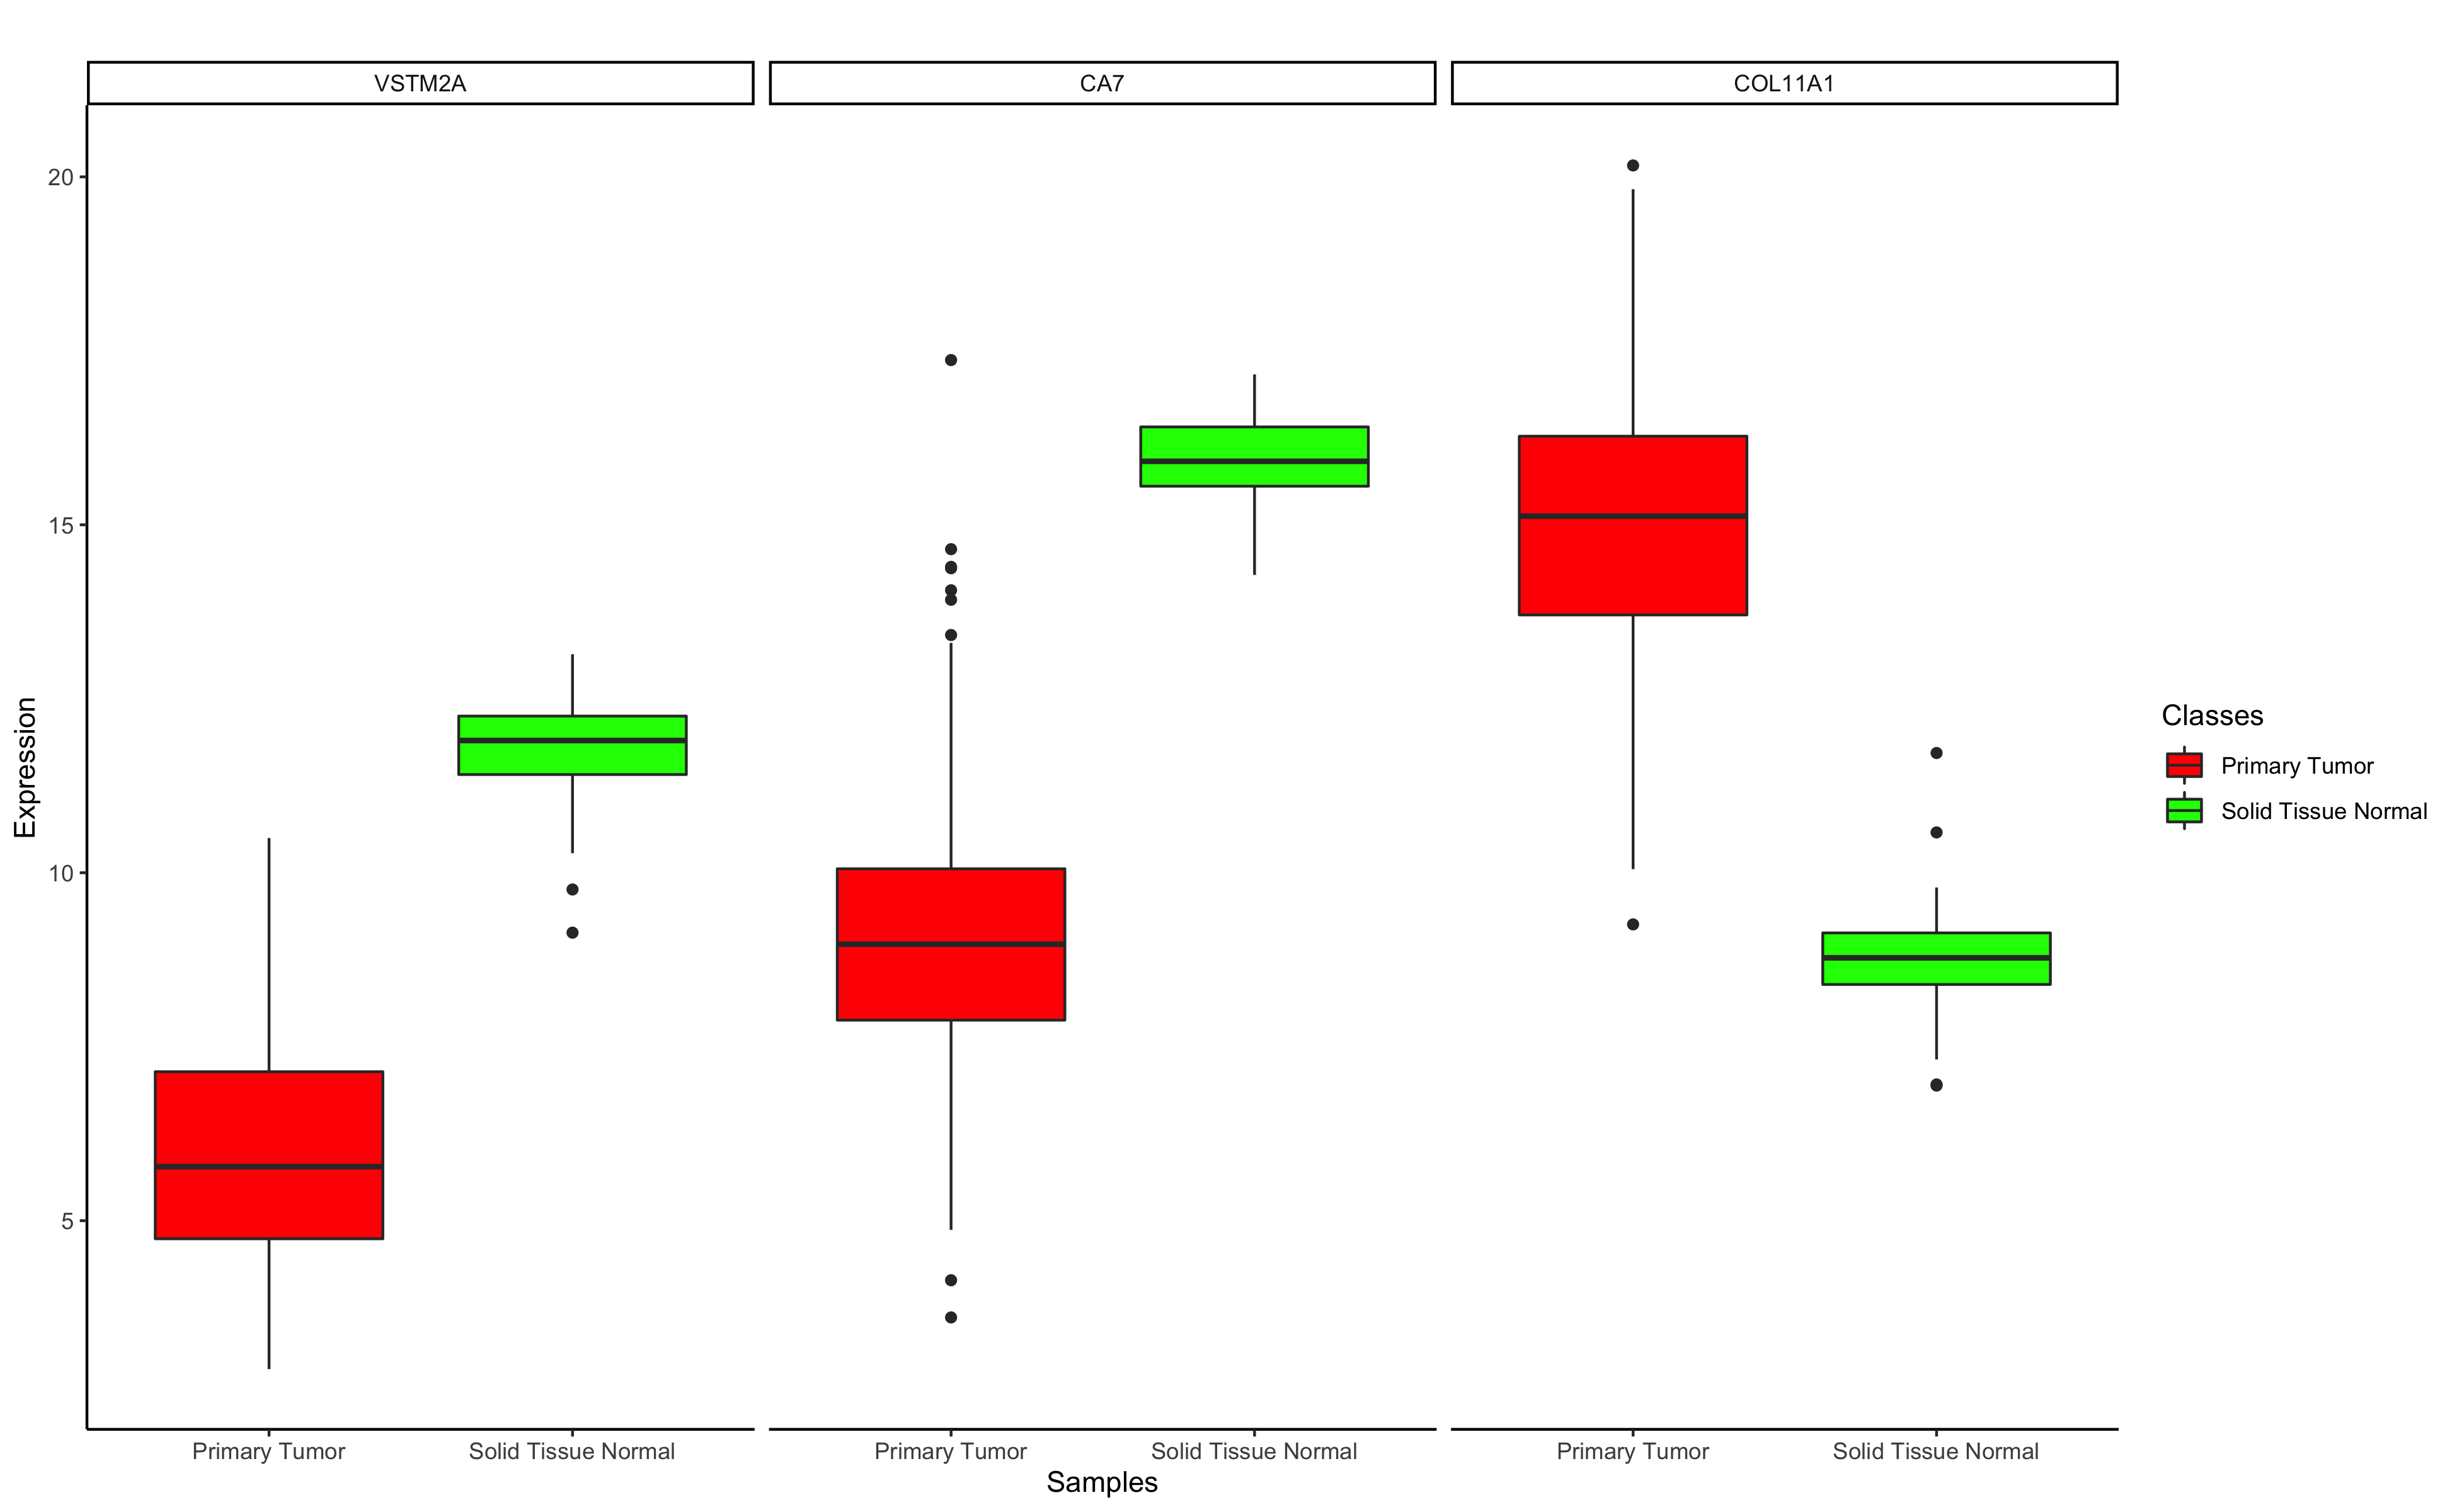
\includegraphics[width=1\textwidth]{figuras/32_cr_biclase_43_knn_boxplots_mejor_metodo.png} 
\end{center}

\newpage
\begin{center}
\textbf{Figura 33}. Diagrama de caja de expresión de genes por tipo de muestra en los 4 genes más relevantes con mRMR como método de selección de características.
\end{center}
\begin{center}
	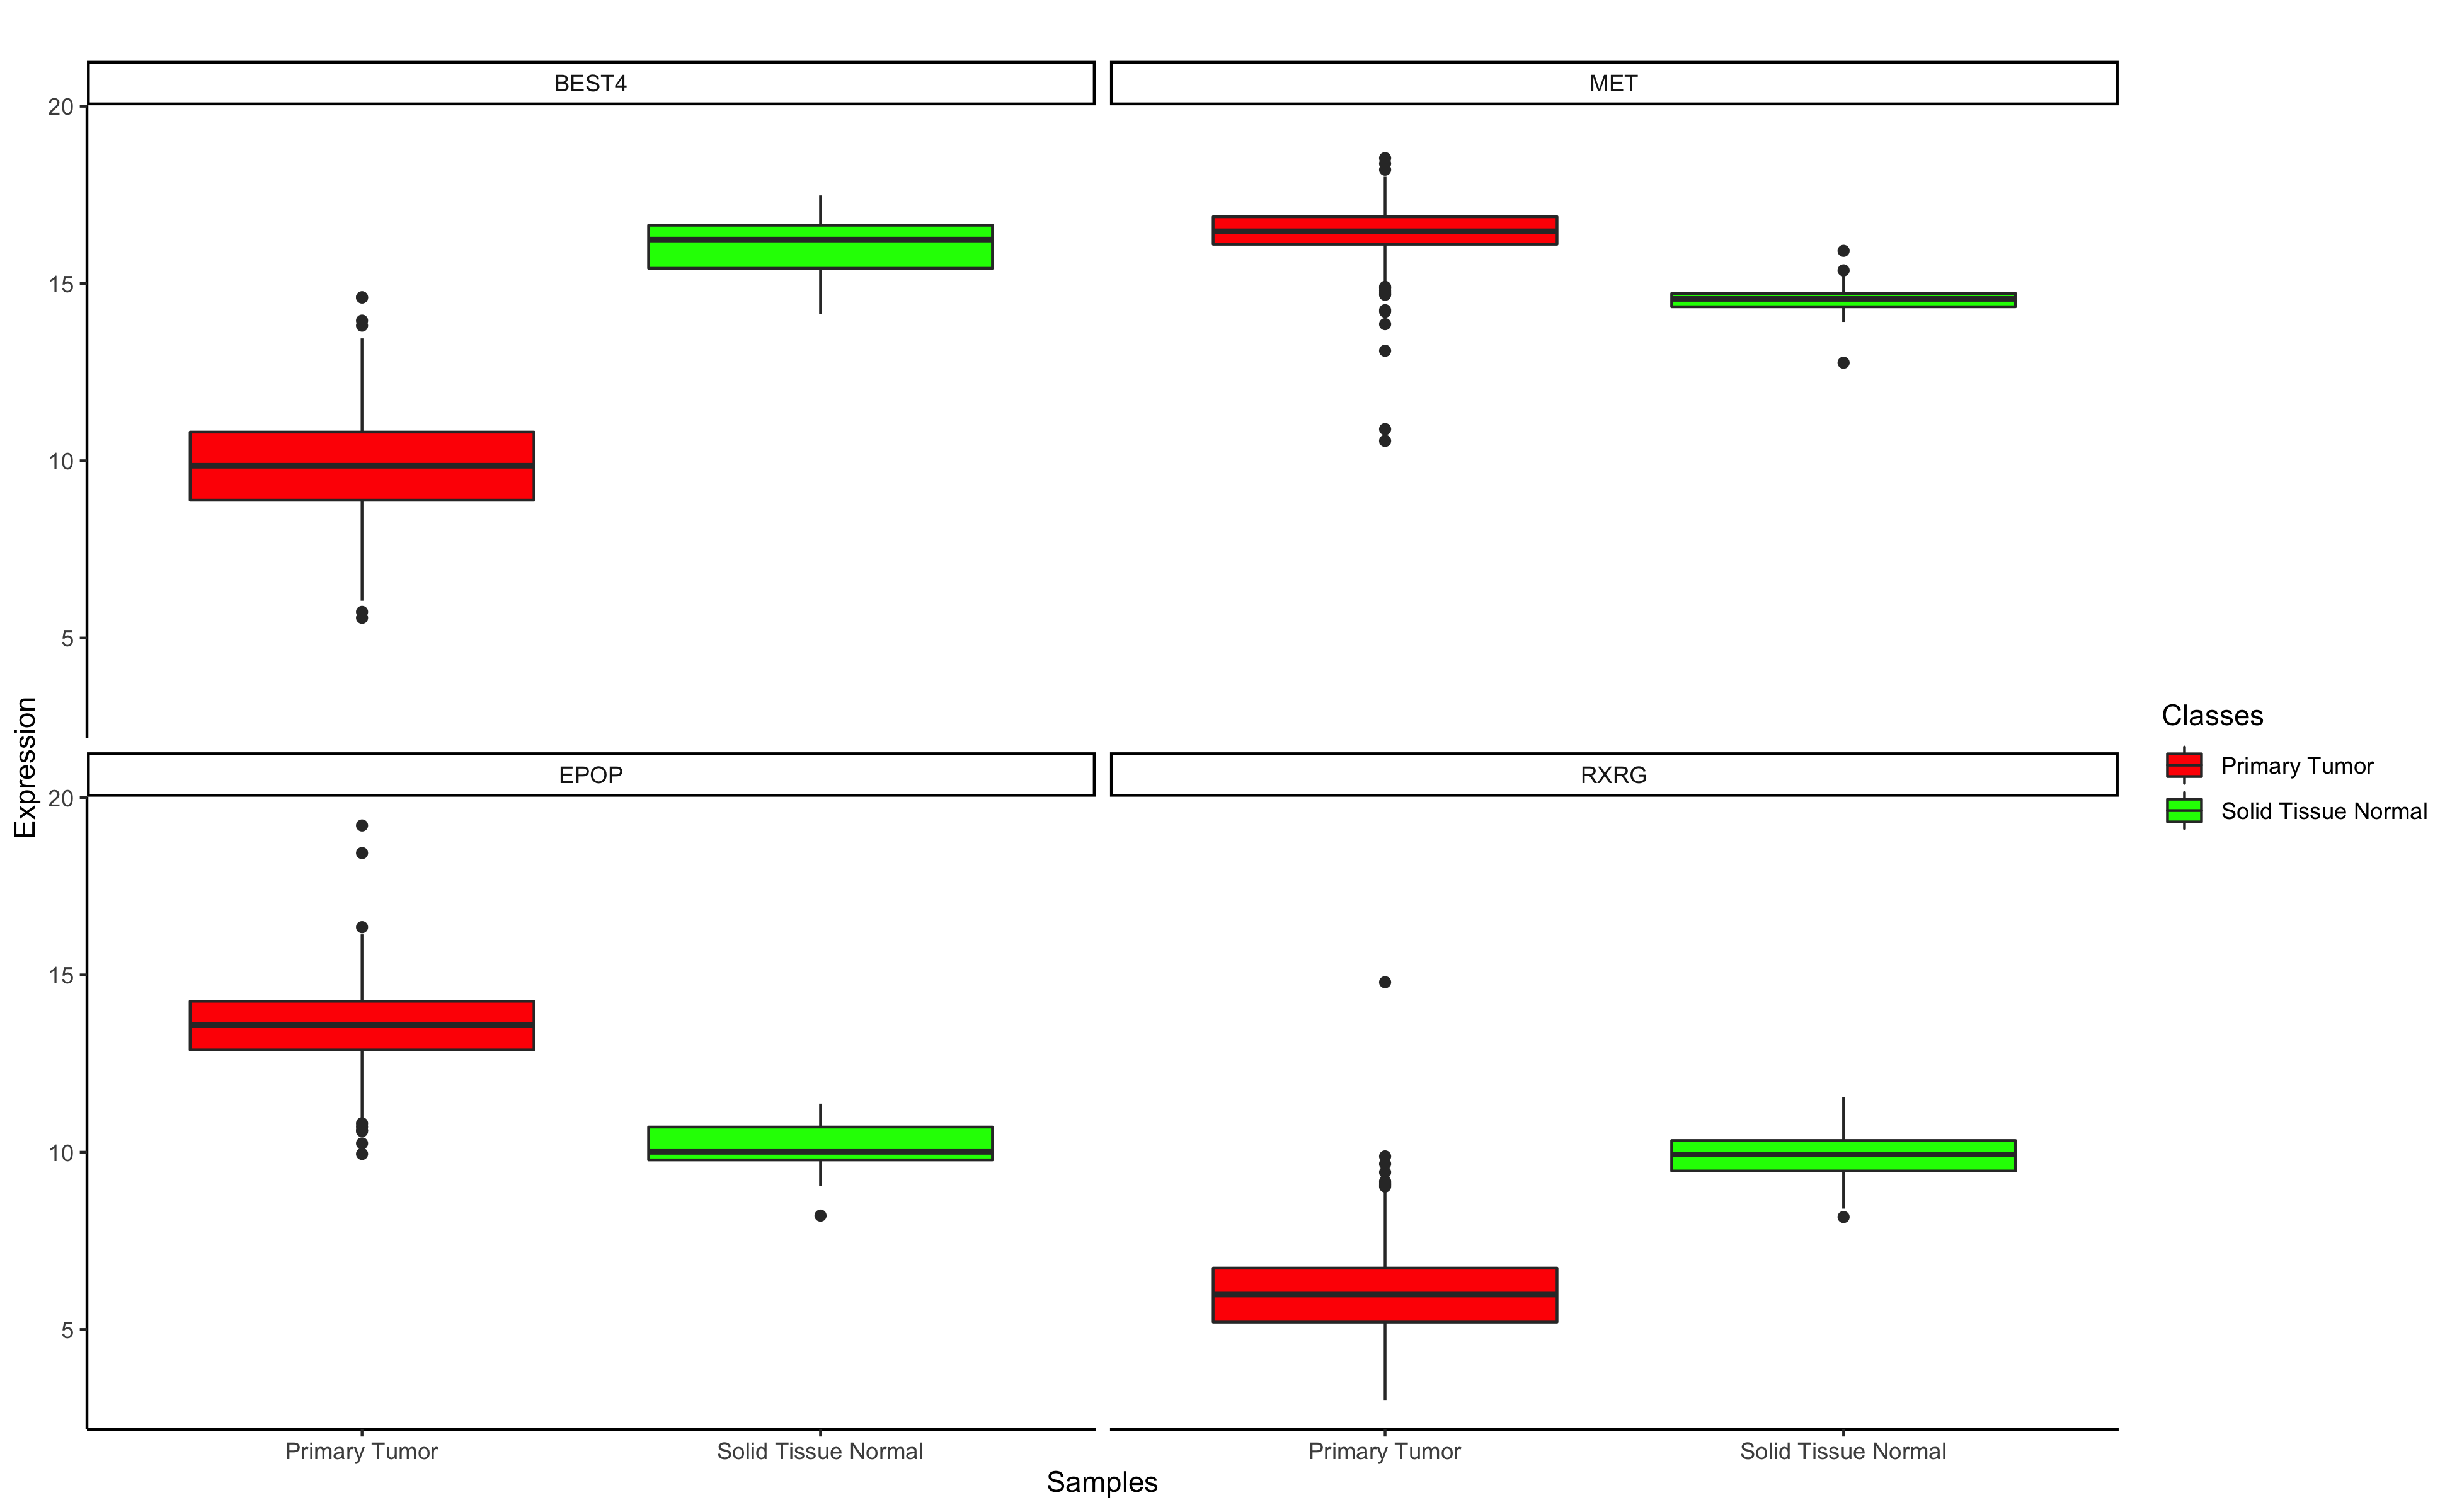
\includegraphics[width=1\textwidth]{figuras/33_cr_biclase_30_rf_boxplots_mejor_metodo.png} 
\end{center}

\subsection{Validación en test}

Al validar en el conjunto de test los mejores modelos encontrados para SVM (dos modelos: 3 genes con mRMR y 3 genes con RF), RF (4 genes con mRMR) y kNN (3 genes con RF) se obtiene la misma clasificación: una predicción perfecta en test (F1-Score 100\%, precisión 100\%) como se muestra en la Figura 34.\\

\newpage
\begin{center}
\textbf{Figura 34}. Matriz de confusión de los mejores modelos encontrados de SVM, RF y kNN en el conjunto de test.
\end{center}

\begin{center}
	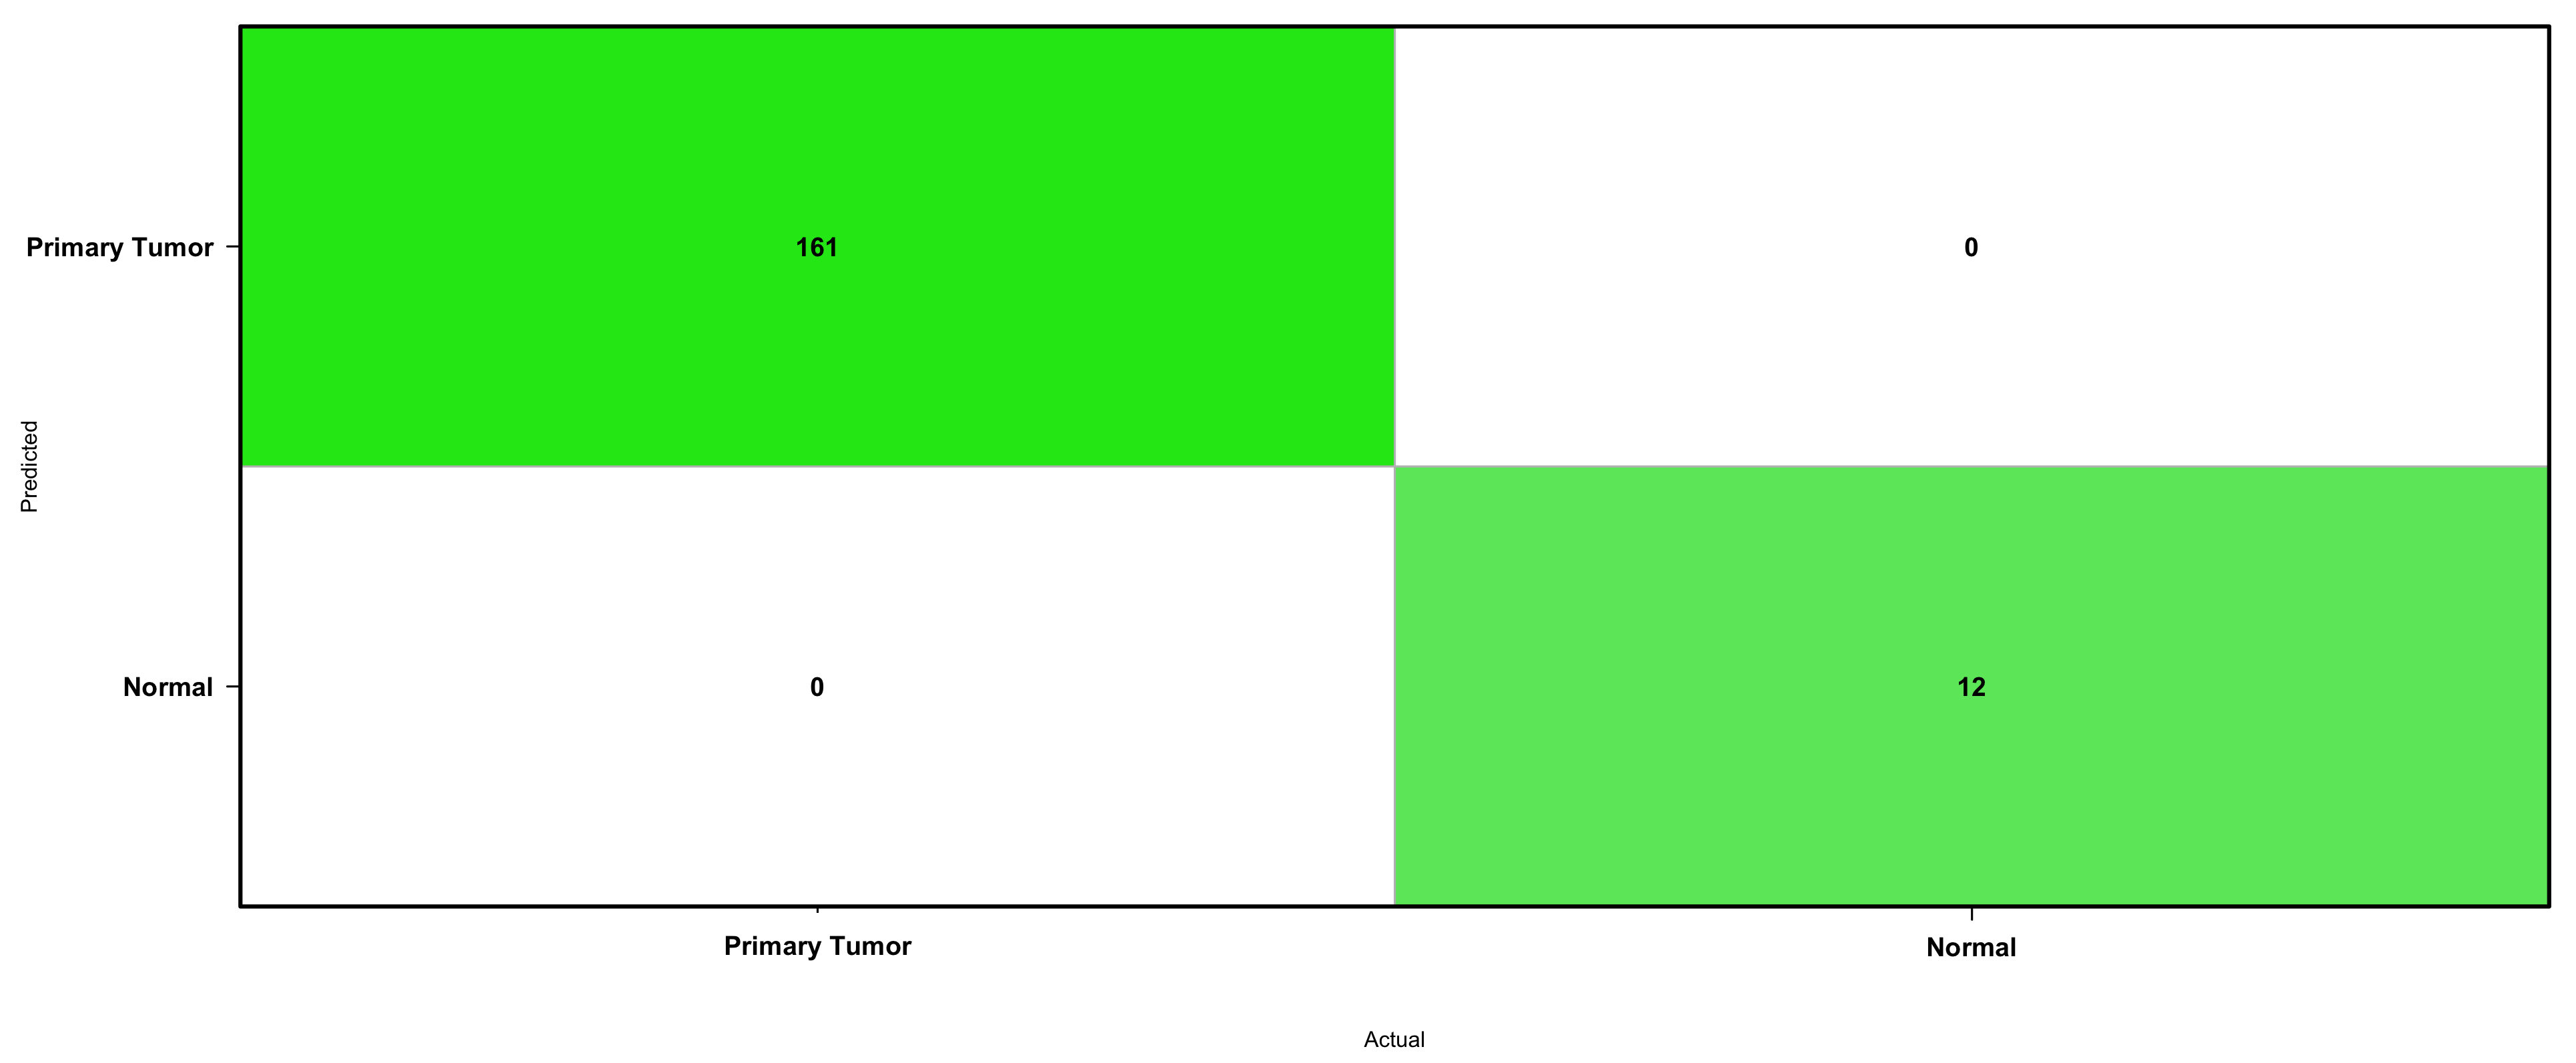
\includegraphics[width=1\textwidth]{figuras/34_cr_biclase_18_svm_matriz_confusion_mejor_metodo.png} 
\end{center}

En la Tabla 31 se muestra un resumen de los mejores modelos obtenidos y su F1-Score y precisión en conjunto de entrenamiento y conjunto de test.\\

\textbf{Tabla 31}. Resumen de clasificación biclase para cáncer de colon-recto. Mejor modelo encontrado para SVM, RF y kNN con biomarcadores seleccionados, parámetros optimizados para cada algoritmo, F1-Score y precisión (Acc) en conjunto de entrenamiento y conjunto de test.

\begin{table}[H]
	\centering
	\begin{tabular}{ccccc|cc}
		\hline
		& Biomarcadores & Parámetros                                                           & F1 train & Acc train & F1 test & Acc test \\ \hline
		\multirow{3}{*}{SVM} &  \textbf{3 genes} mRMR & \begin{tabular}[c]{@{}c@{}}$c$ = 0,05\\ $\gamma$ = 0,06\end{tabular} & 100      & 100       & 100     & 100      \\ \cline{2-7} 
		& \textbf{3 genes}  RF   & \begin{tabular}[c]{@{}c@{}}$c$ = 0,05\\ $\gamma$ = 0,07\end{tabular} & 100      & 100       & 100     & 100      \\ \hline
		RF                   &  \textbf{4 genes} mRMR  & --                                                                   & 100      & 100       & 100     & 100      \\ \hline
		kNN                  & \textbf{3 genes} RF    & k = 23                                                               & 100      & 100       & 100     & 100      \\ \hline
	\end{tabular}
\end{table}

\subsection{Conclusiones}

Como principal conclusión, los mejores modelos de SVM, RF y kNN distinguen perfectamente entre tejido tumoral y tejido sano utilizando menos de 5 genes en todos los casos.\\

En la plataforma de Open Targets \cite{OpenTargets2020} se encuentra asociación entre todos los genes de los mejores modelos (4 mejores genes de mRMR y 3 mejores genes de RF) y el cáncer de colon-recto.

\section{Resultados de clasificación multiclase para cáncer de colon-recto}

El código completo del análisis se muestra en el fichero \textit{\texttt{analisis\_cr/\linebreak04\_analisis\_multiclase.R}} del repositorio de GitHub asociado al trabajo \cite{Redondo-Sanchez2020}.

\subsection{Detección de biomarcadores}

Para la clasificación multiclase en cáncer de colon-recto se cuenta con 530 adenocarcinomas, 87 adenocarcinomas mucinosos y 51 muestras de tejido sano (Tabla 32).\\

\textbf{Tabla 32}. Distribución de tipos de muestra para el análisis de cáncer de colon-recto multiclase.

\begin{table}[H]
	\centering
	\begin{tabular}{lcc}
		\cline{2-3}
		& \textbf{Número de casos} & \textbf{Porcentaje} \\ \hline
		\textbf{Adenocarc.}          & 530 & 79,3\%  \\
		\textbf{Adenocarc. muc.} & 87  & 13,0\%  \\
		\textbf{Tejido normal}           & 51  & 7,6\%   \\ \hline
		\textbf{Total}                   & 668 & 100,0\%
	\end{tabular}
\end{table}

Se extraen 6.848 genes que presentan en su expresión diferencias significativas entre las distintas muestras de tumores y las de tejido sano. En la Tabla 33 se muestra la partición entrenamiento - test realizada y en la figura 35 se representa en un diagrama de Sankey.\\

\newpage
\textbf{Tabla 33}. Distribución entrenamiento-test según tipo de muestra y proporción entre clases para el análisis de colon-recto multiclase.

\begin{table}[H]
	\centering
	\begin{tabular}{lccc}
		\cline{2-4}
		\multicolumn{1}{c}{\textbf{}}                                                    & \textbf{Total} & \textbf{Entrenamiento} & \textbf{Test} \\ \hline
		\textbf{Adenocarc.}                                                          & 530 (100\%)    & 398 (75,1\%)           & 132 (24,9\%)  \\
		\textbf{Adenocarc. muc.}       & 87 (100\%)     & 66 (75,9\%)            & 21 (24,1\%)   \\
		\textbf{Tejido sano}                                                             & 51 (100\%)     & 39 (76,5\%)            & 12 (23,5\%)   \\ \hline
		\textbf{\begin{tabular}[c]{@{}l@{}}Proporción\\ adenoc./sanos\end{tabular}}      & 10,4           & 10,2                   & 11,0          \\
		\textbf{\begin{tabular}[c]{@{}l@{}}Proporción\\ adenoc. muc./sanos\end{tabular}} & 1,7            & 1,7                    & 1,8           \\ \hline
	\end{tabular}
\end{table}

\begin{center}
\textbf{Figura 35}. Diagrama de Sankey mostrando la partición entrenamiento-test realizada según tipo de muestra para el análisis de colon-recto multiclase.
\end{center}

\begin{center}
	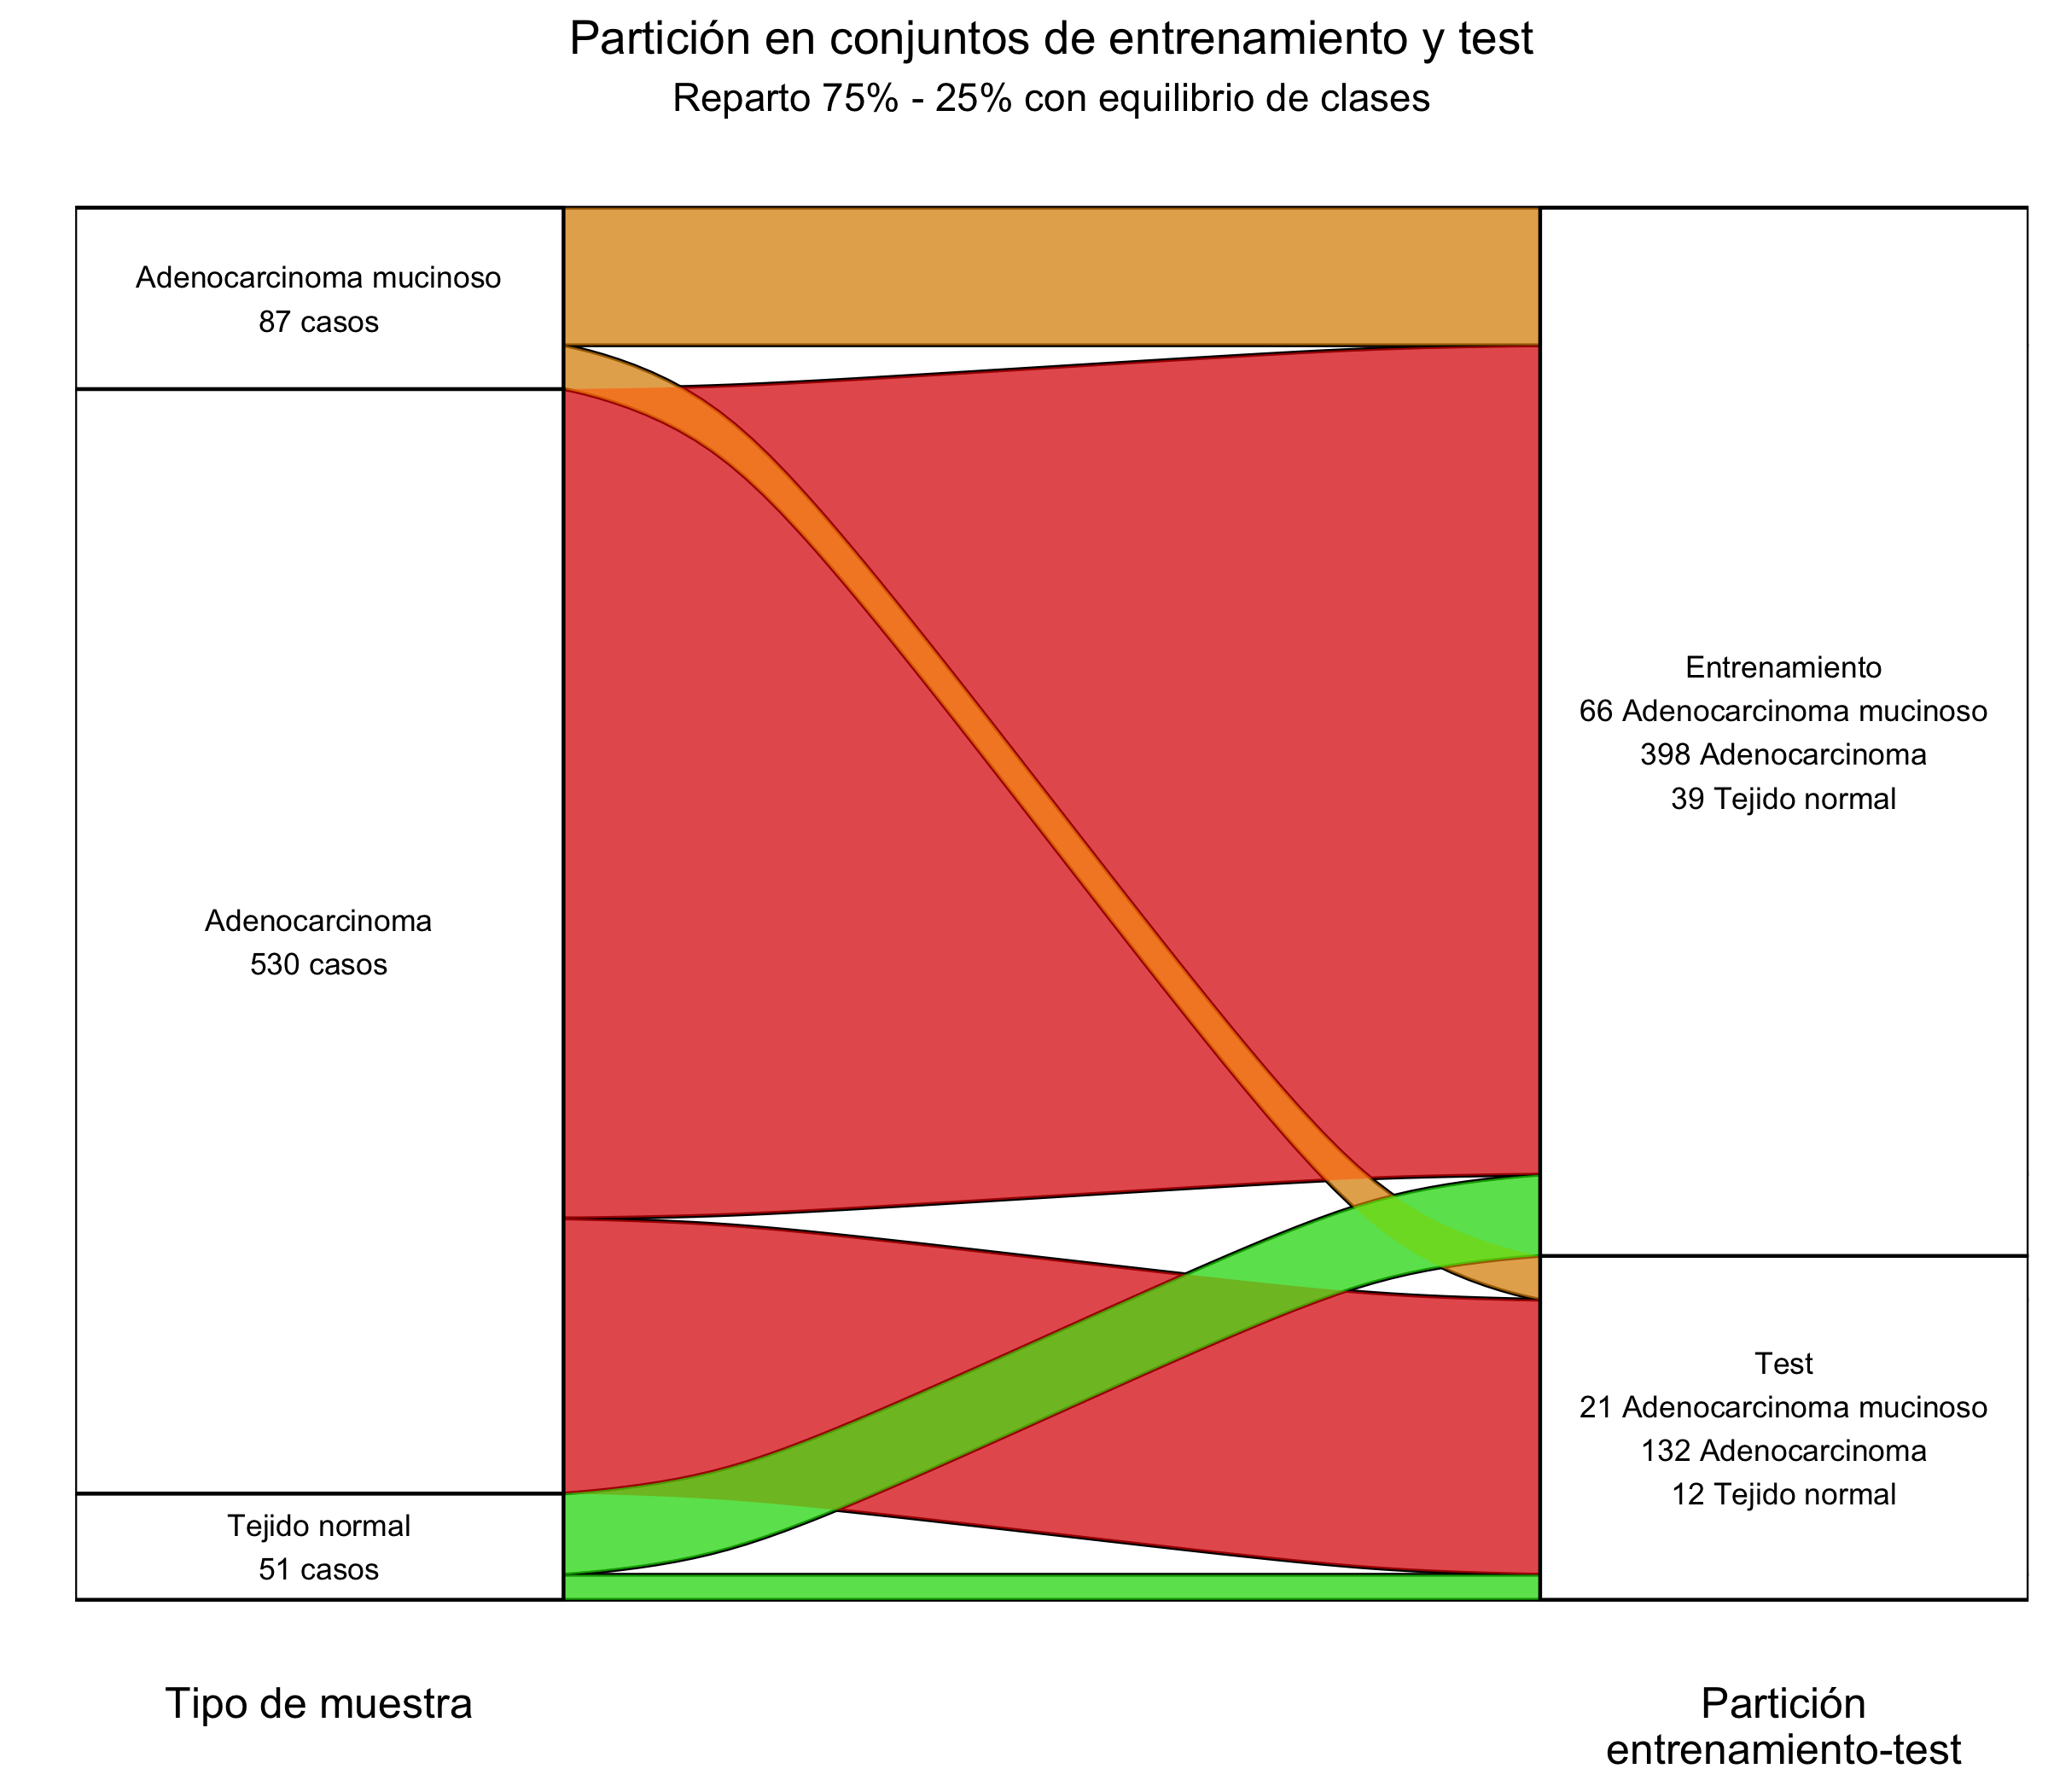
\includegraphics[width=.75\textwidth]{figuras/35_cr_multiclase_05_sankey.png}
\end{center}

\newpage
A continuación se muestran los diez genes más relevantes encontrados por cada método de selección de características:\\

\textbf{Tabla 34}. Diez genes más relevantes según los distintos métodos de selección de características para el análisis de colon-recto multiclase.

\begin{table}[H]
	\centering
	\begin{tabular}{clll}
		\hline
		Ranking & \multicolumn{1}{c}{mRMR} & \multicolumn{1}{c}{RF} & \multicolumn{1}{c}{DA} \\ \hline
		1       & GTF2IRD1                 & COL11A1                & CD79B                  \\
		2       & ESM1                     & GTF2IRD1               & SCN4A                  \\
		3       & MUC2                     & MUC2                   & BTK                    \\
		4       & CLEC3B                   & CSE1L                  & BRCA1                  \\
		5       & KRT80                    & SCGN                   & FAS                    \\
		6       & SLC11A1                  & CA7                    & ROS1                   \\
		7       & OSBPL3                   & PVT1                   & TNFRSF17               \\
		8       & SLC39A10                 & ESM1                   & POLQ                   \\
		9       & GDPD5                    & CPNE7                  & FGFR2                  \\
		10      & CDH3                     & MDFI                   & ATP2B3                 \\ \hline
	\end{tabular}
\end{table}

Los genes GTF2IRD1, ESM1 y MUC2 son comunes a dos algoritmos de selección de características: mRMR y RF.

\subsection{Validación cruzada en entrenamiento}

En las Tablas 35 y 36 se muestran los parámetros óptimos de SVM y kNN obtenidos.\\

\textbf{Tabla 35}. Parámetros óptimos de SVM encontrados para los 10 genes más relevantes de cada método de selección de características.

\begin{table}[H]
	\centering
	\begin{tabular}{cccc}
		\hline
		\textbf{Parámetro} & \textbf{mRMR} & \textbf{RF} & \textbf{DA} \\ \hline
		Coste                &    0,5 &    5     &  2       \\
		Gamma               &     0,1   &     0,07   & 0,08        \\ \hline
	\end{tabular}
\end{table}

\textbf{Tabla 36}. Número óptimo de vecinos encontrado para los 10 genes más relevantes de cada método de selección de características.

\begin{table}[H]
	\centering
	\begin{tabular}{cccc}
		\cline{2-4}
		\textbf{} & \textbf{mRMR} & \textbf{RF} & \textbf{DA} \\ \hline
		k                &   19 &   7     &   23      \\ \hline
	\end{tabular}
\end{table}

En la Figura 36 se muestran para SVM, RF y kNN el F1-Score medio obtenido en las 5 fold.

\begin{center}
	\textbf{Figura 36}. Mapa de calor con valores medios y desviación típica de los 5-fold de F1-Score de SVM, RF y kNN según método de selección de características y número de genes usados.
\end{center}
\begin{center}
	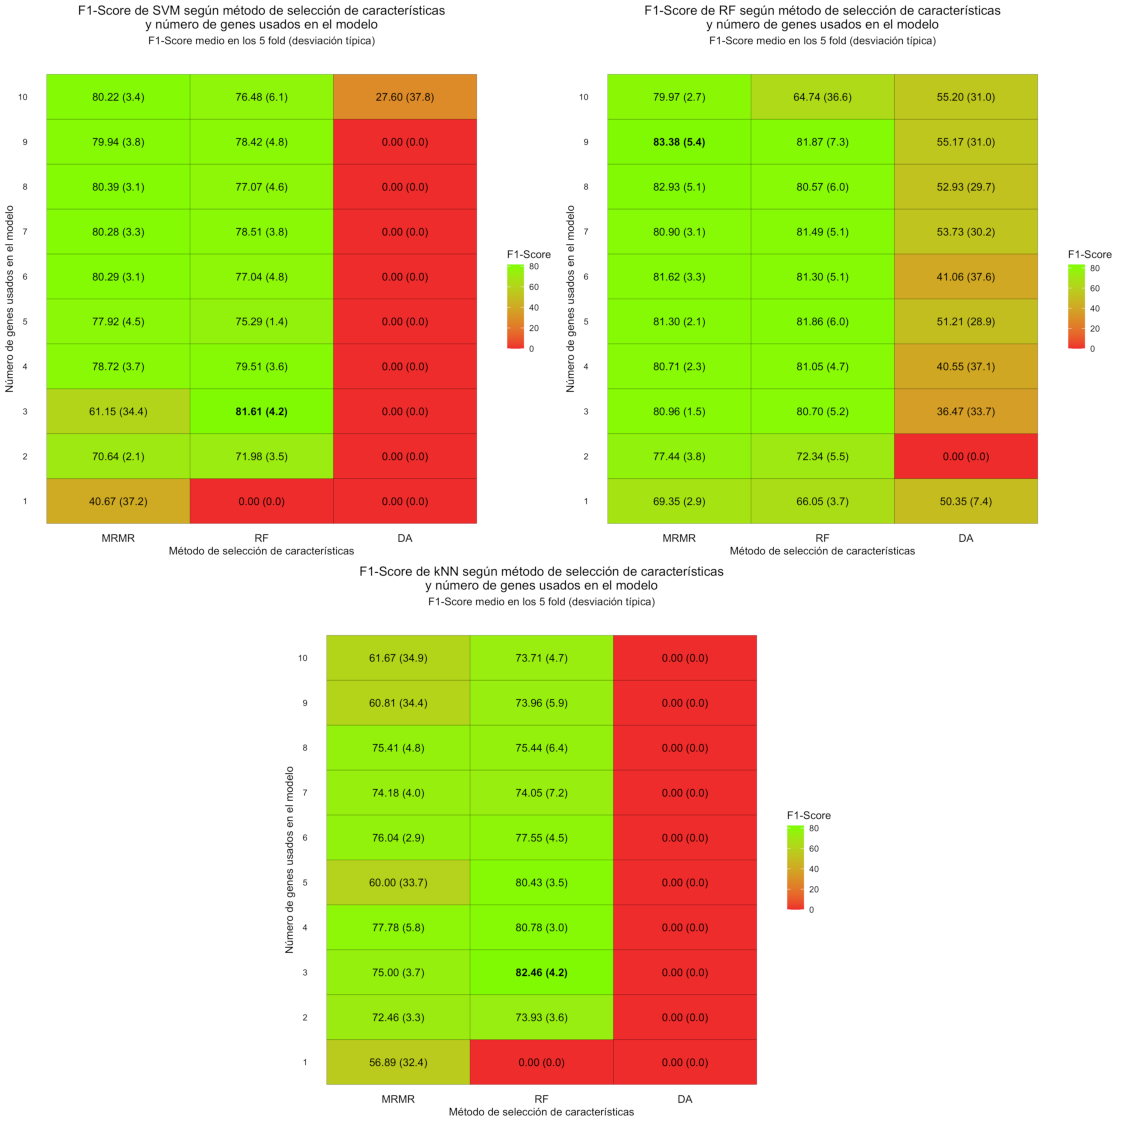
\includegraphics[width=1\textwidth]{figuras/36_cr_multiclase_heatmap_horizontal.pdf} 
\end{center}

El F1-Score es bastante inferior al obtenido en el resto de análisis. Los mejores modelos son:
\begin{itemize}
	\item Para SVM y kNN: RF con 3 genes.
	\item Para RF: mRMR con 9 genes.
\end{itemize}

Se analiza la expresión de 3 genes más relevantes de RF y los 9 más relevantes de mRMR con diagramas de caja (Figuras 37 y 38).

\begin{center}
	\textbf{Figura 37}. Diagrama de caja de expresión de genes por tipo de muestra en los 3 genes más relevantes con RF como método de selección de características.
\end{center}
\begin{center}
	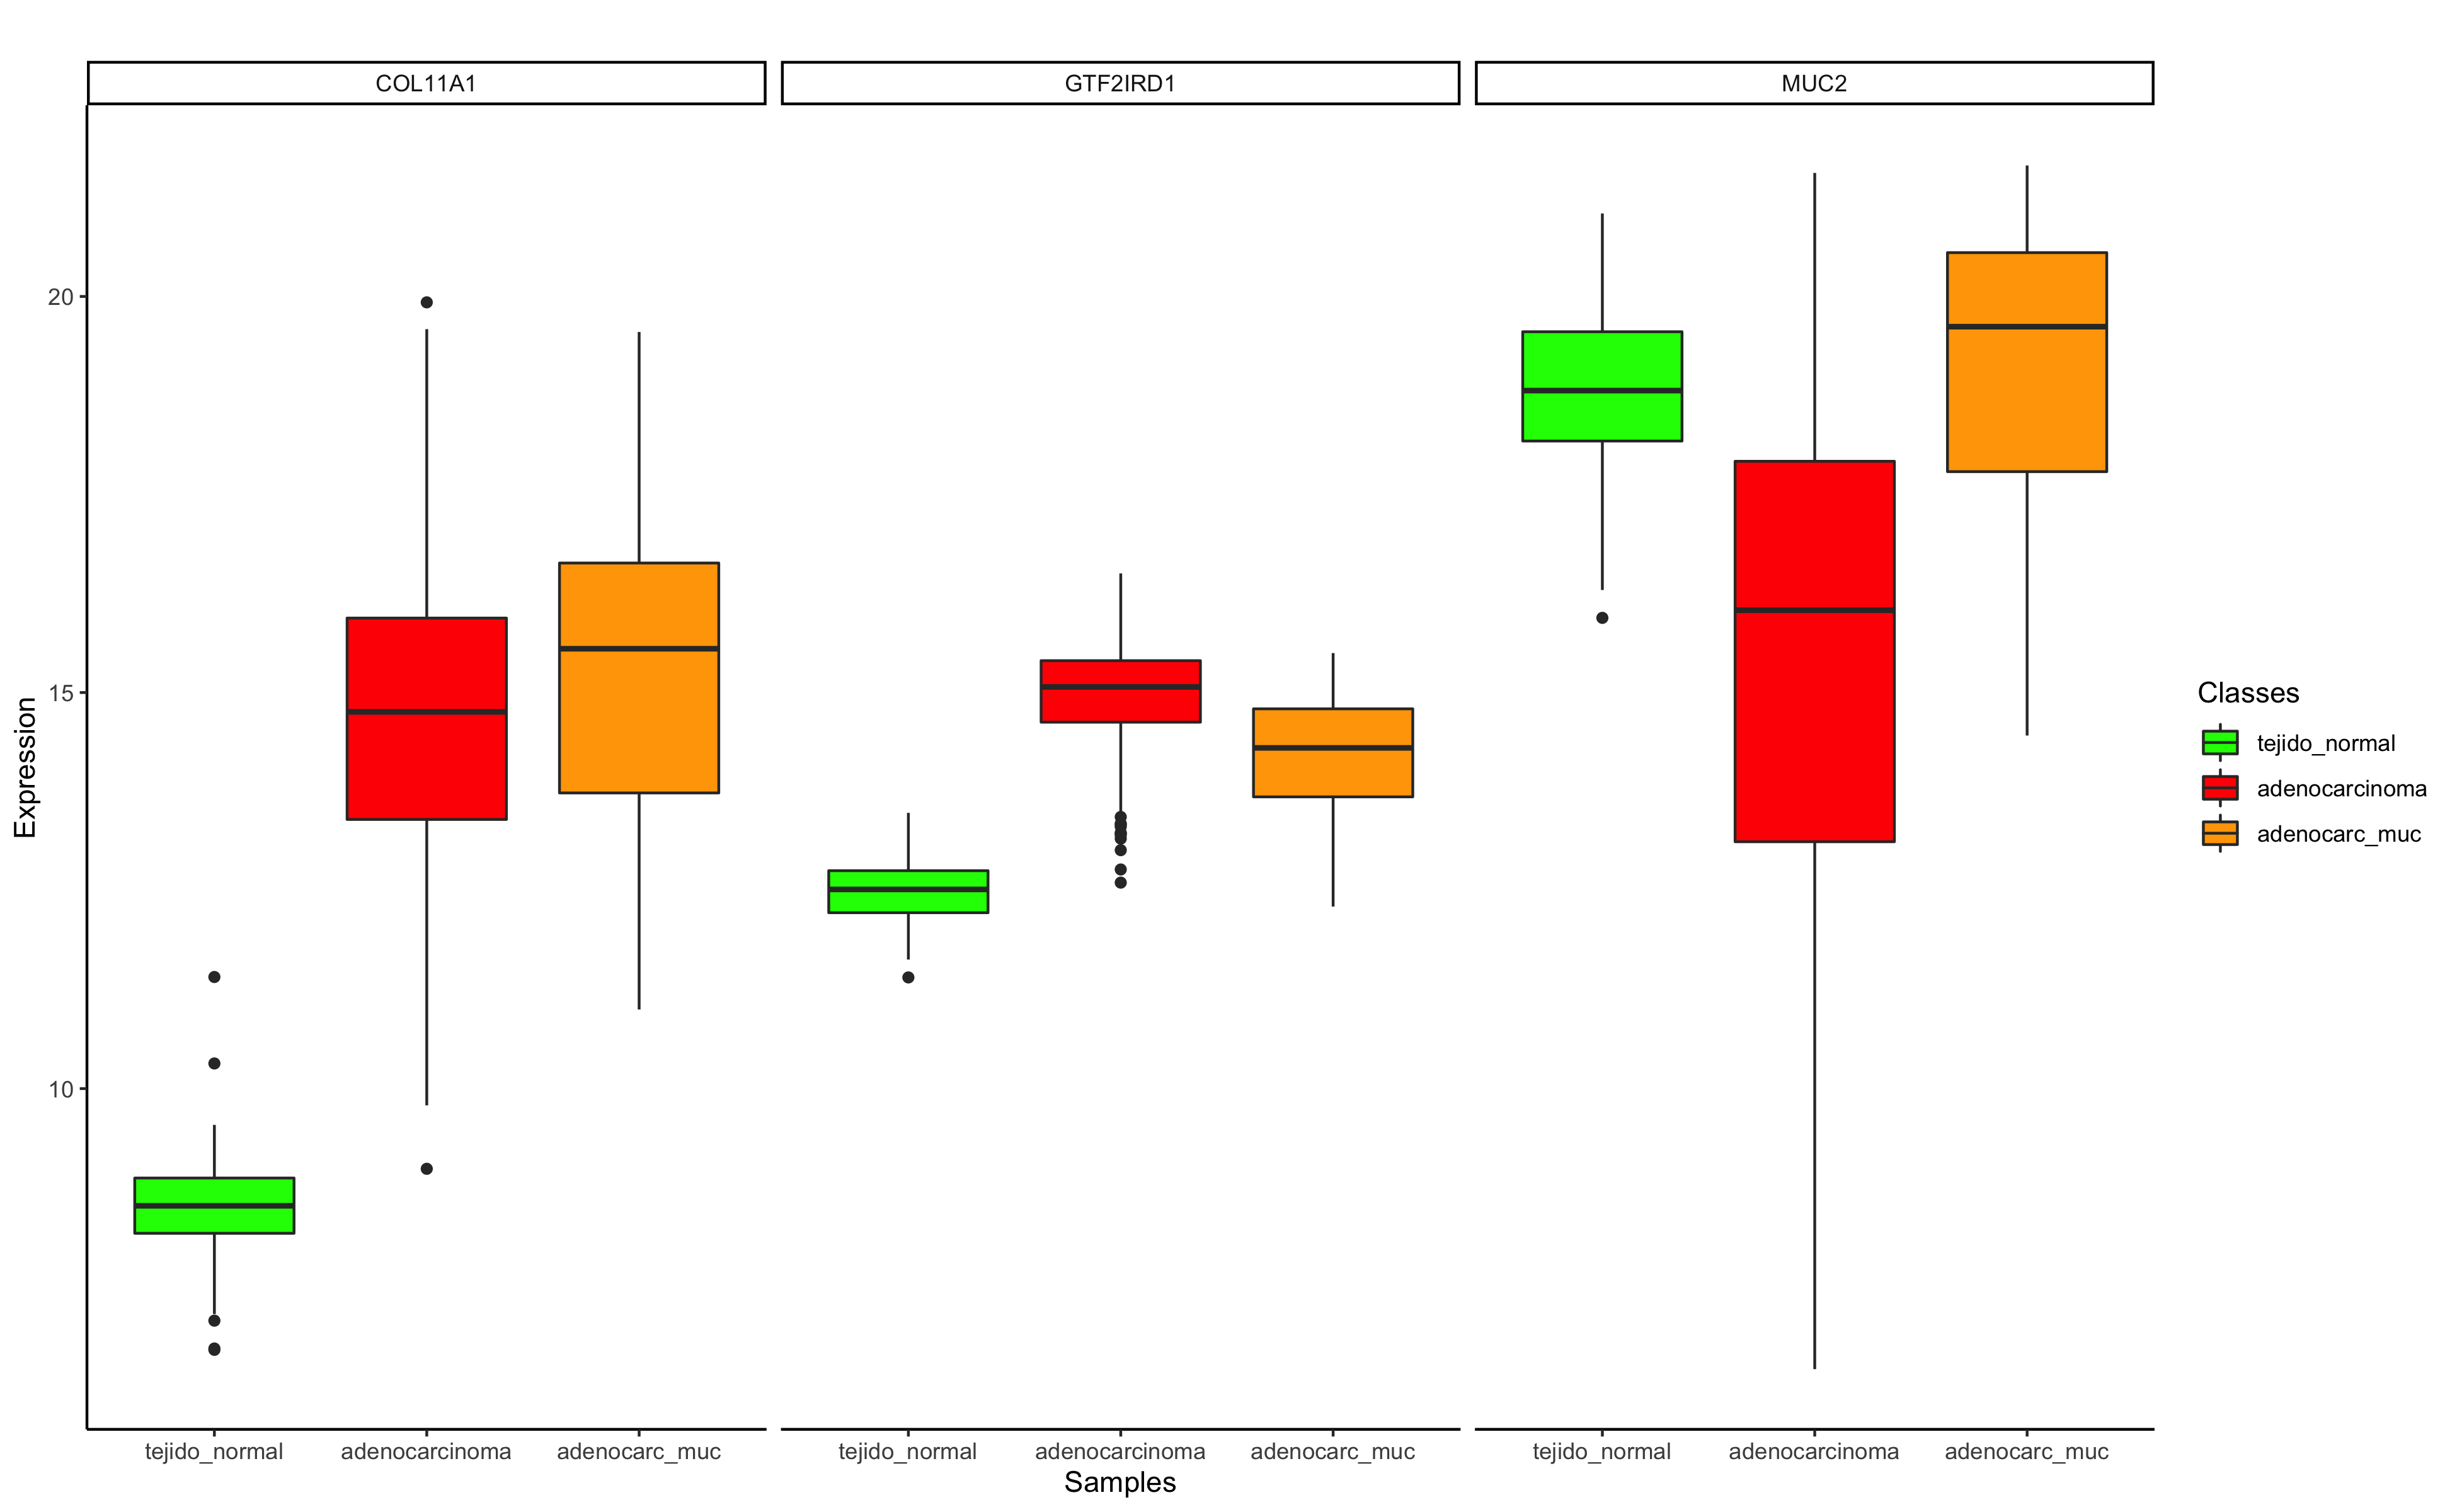
\includegraphics[width=1\textwidth]{figuras/37_cr_multiclase_34_knn_boxplots_mejor_metodo.png} 
\end{center}

\newpage
\begin{center}
	\textbf{Figura 38}. Diagrama de caja de expresión de genes por tipo de muestra en los 9 genes más relevantes con mRMR como método de selección de características.
\end{center}
\begin{center}
	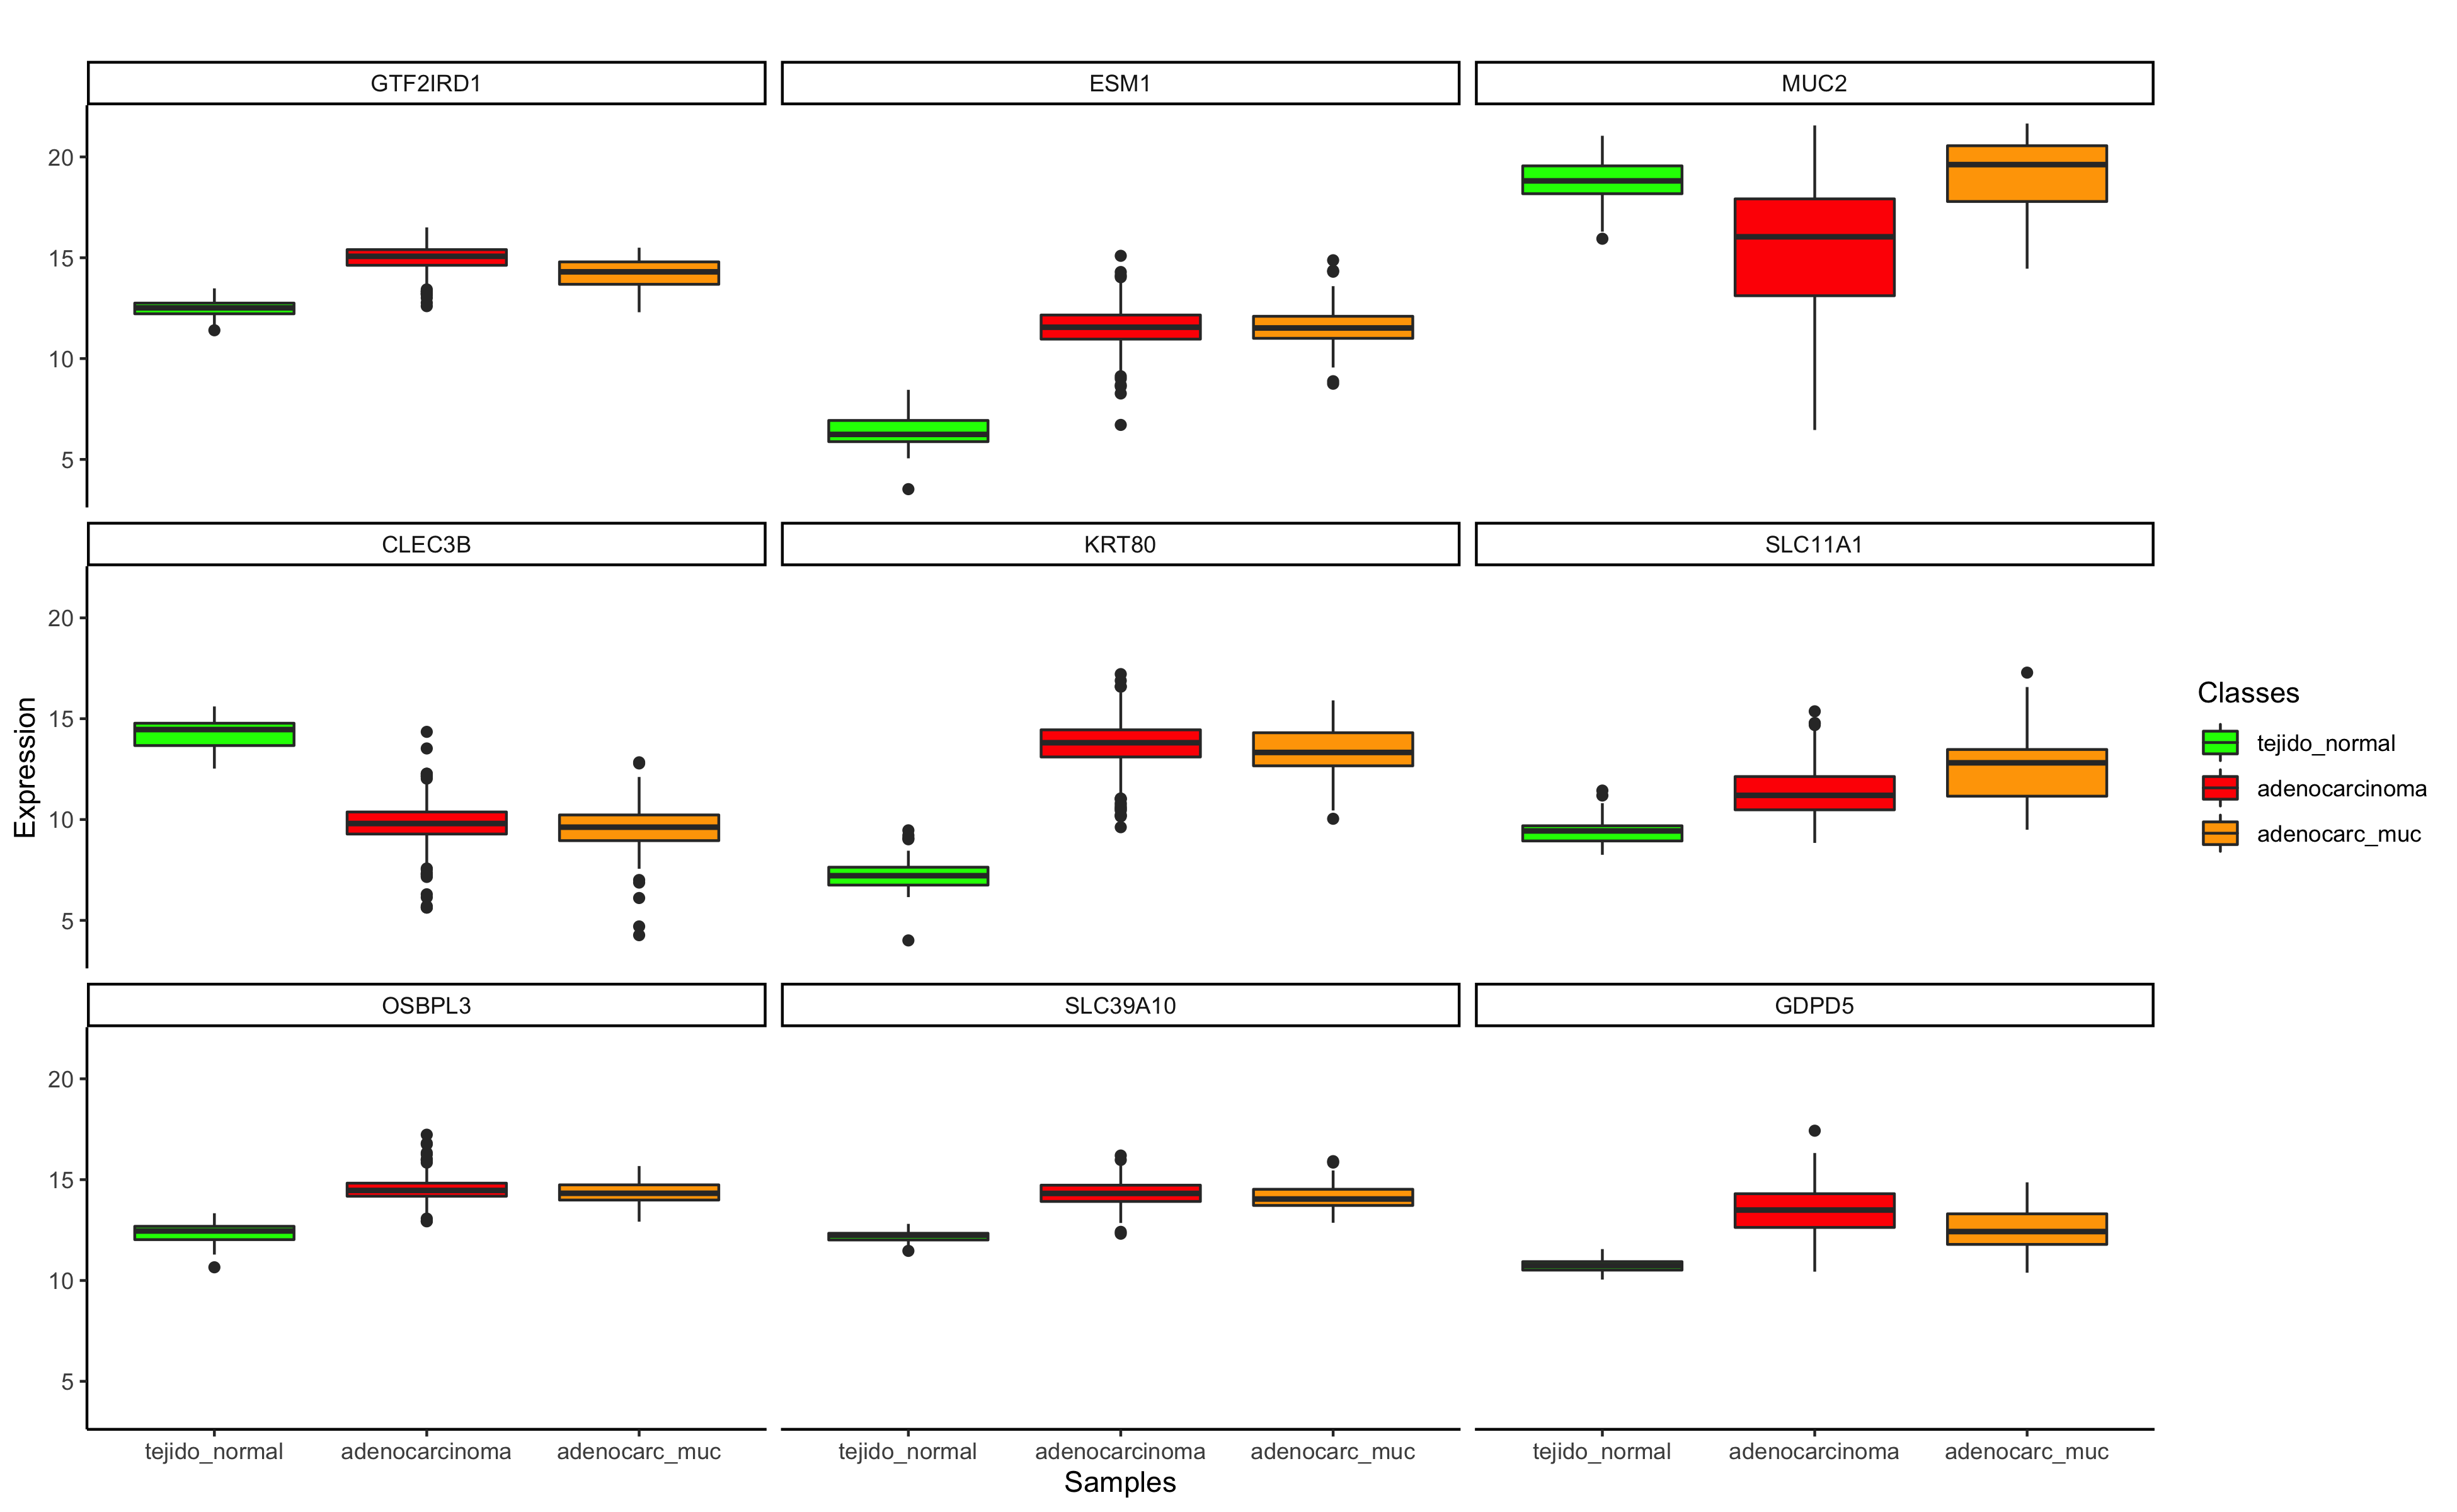
\includegraphics[width=1\textwidth]{figuras/38_cr_multiclase_24_rf_boxplots_mejor_metodo.png} 
\end{center}

\subsection{Validación en test}

Al validar en el conjunto de test los mejores modelos encontrados para SVM (3 genes con RF), RF (9 genes con mRMR) y kNN (3 genes con RF) se obtienen las matrices de confusión mostradas en las Figuras 39, 40 y 41, respectivamente.

\newpage
\begin{center}
	\textbf{Figura 39}. Matriz de confusión del mejor modelo encontrado de SVM en el conjunto de test.
\end{center}
\begin{center}
	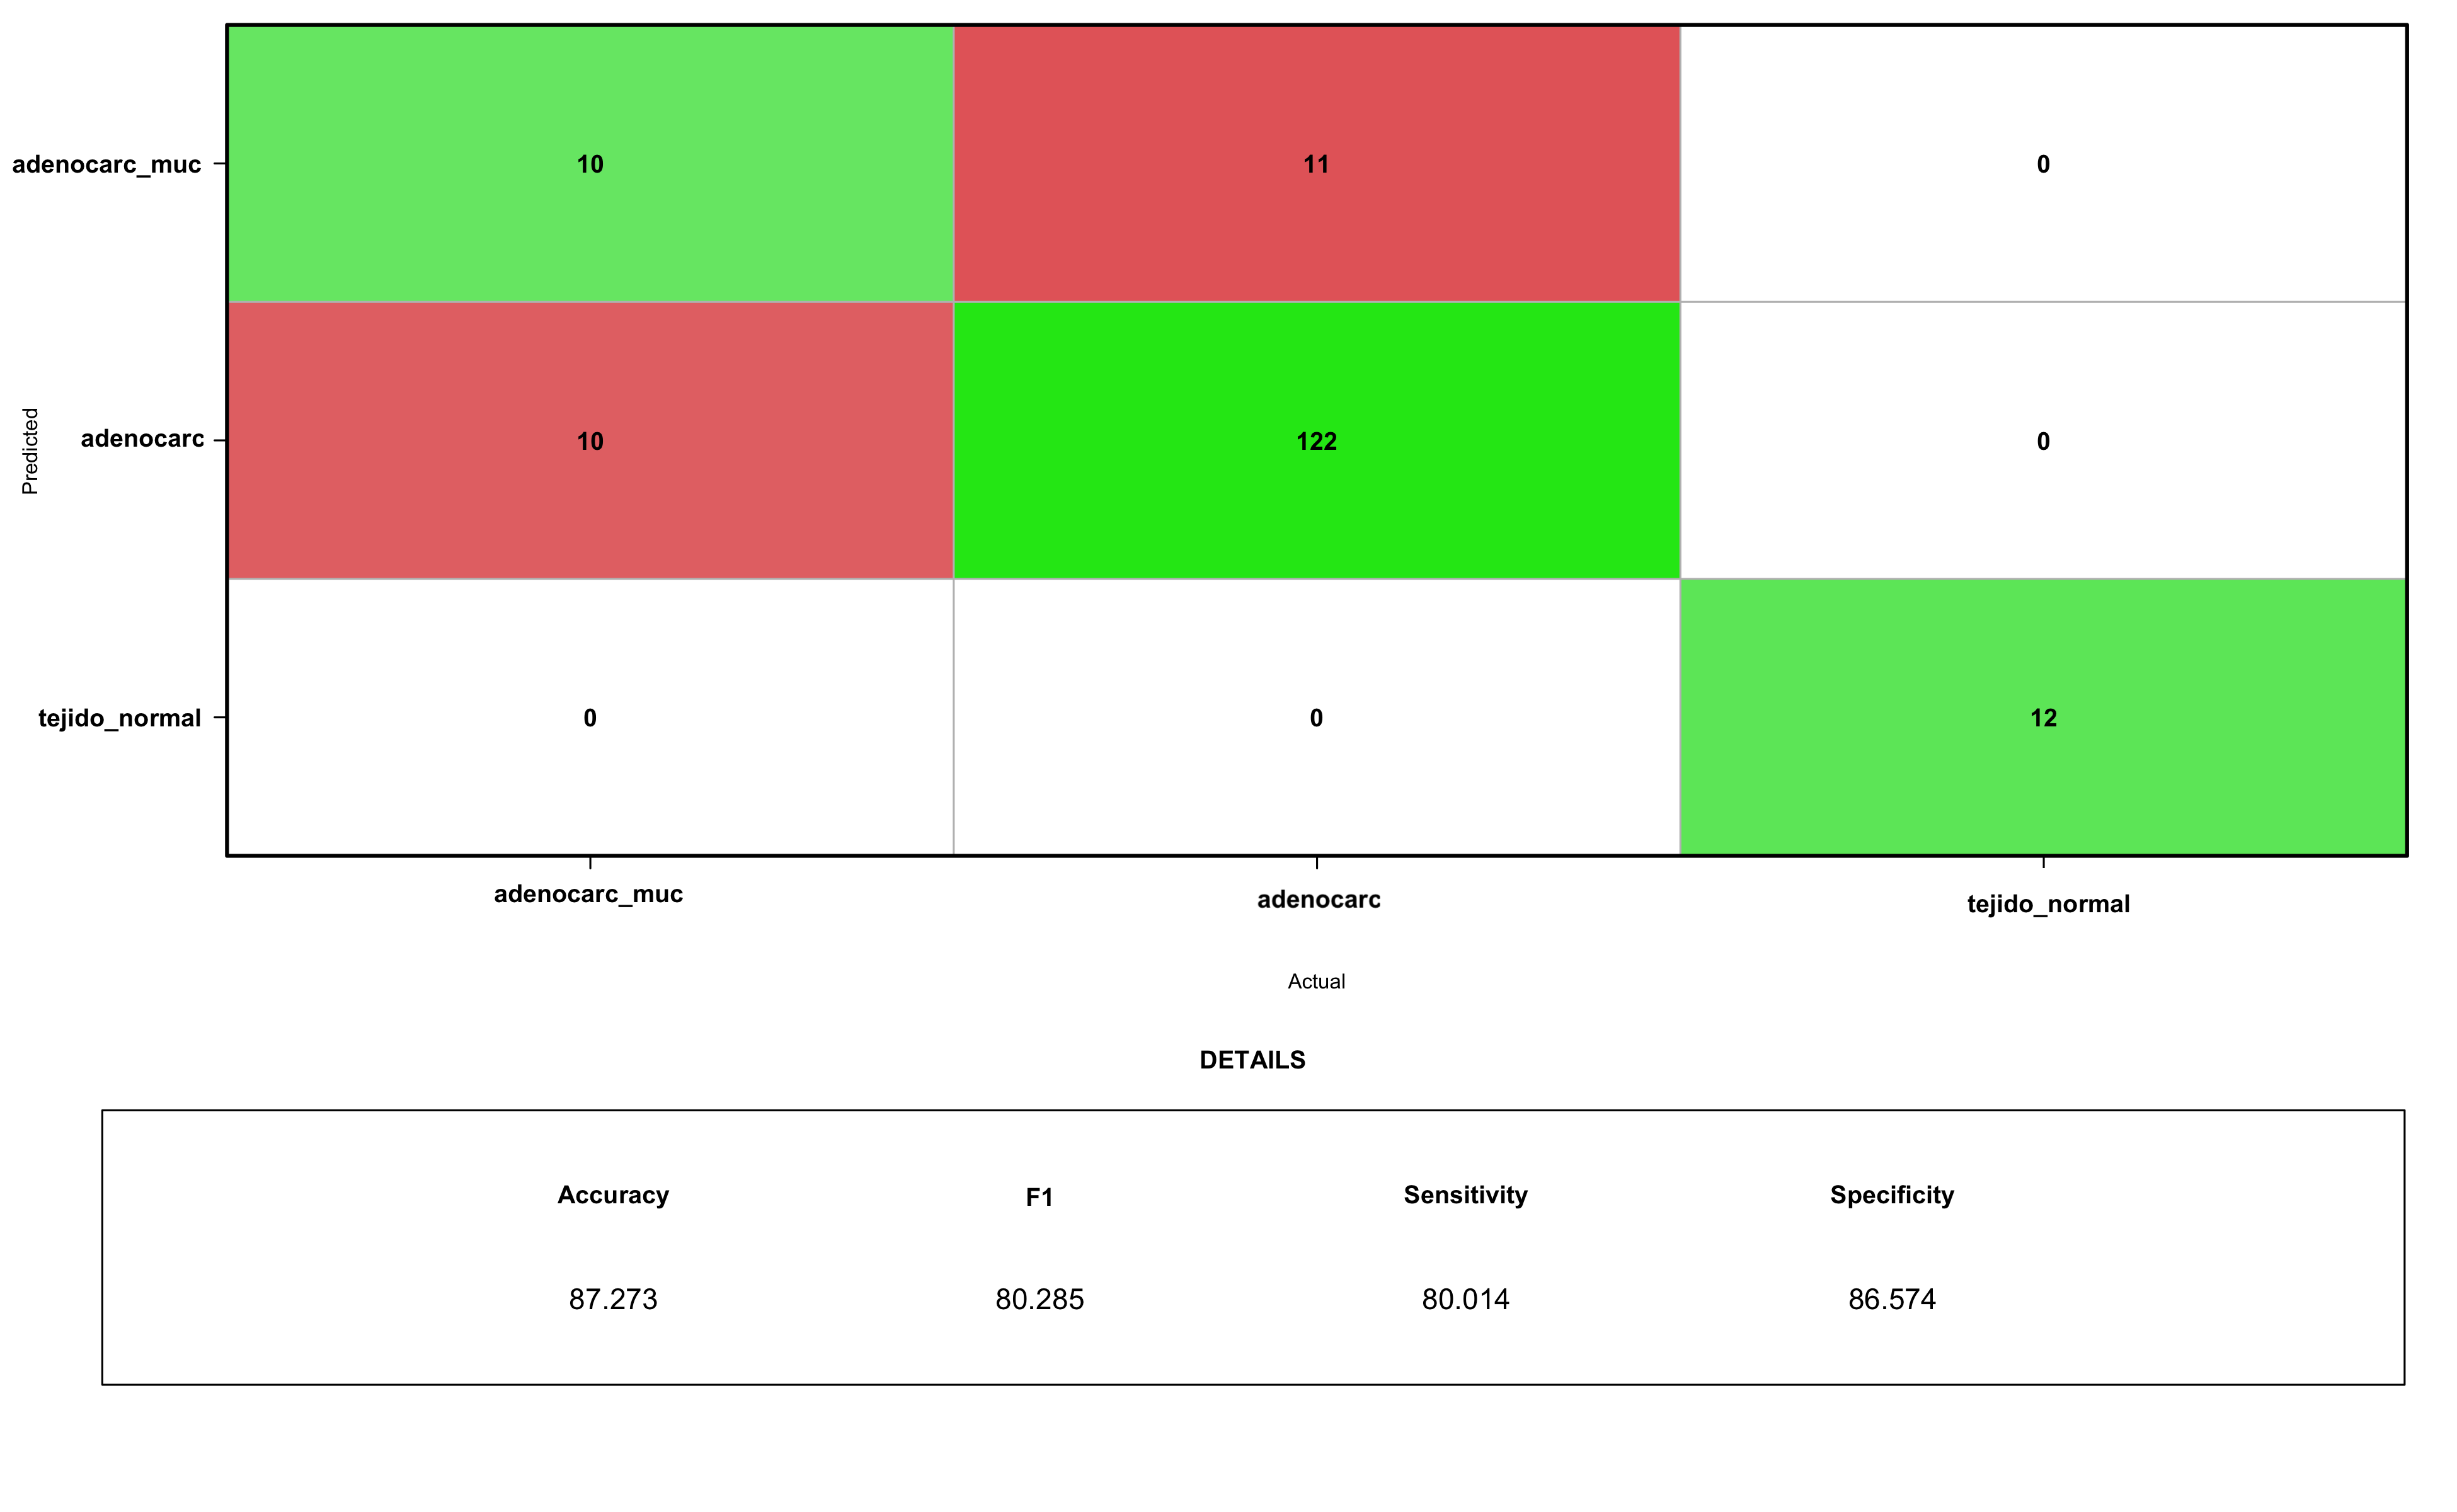
\includegraphics[width=1\textwidth]{figuras/39_cr_multiclase_15_svm_matriz_confusion_mejor_metodo.png} 
\end{center}

\begin{center}
	\textbf{Figura 40}. Matriz de confusión del mejor modelo encontrado de RF en el conjunto de test.
\end{center}
\begin{center}
	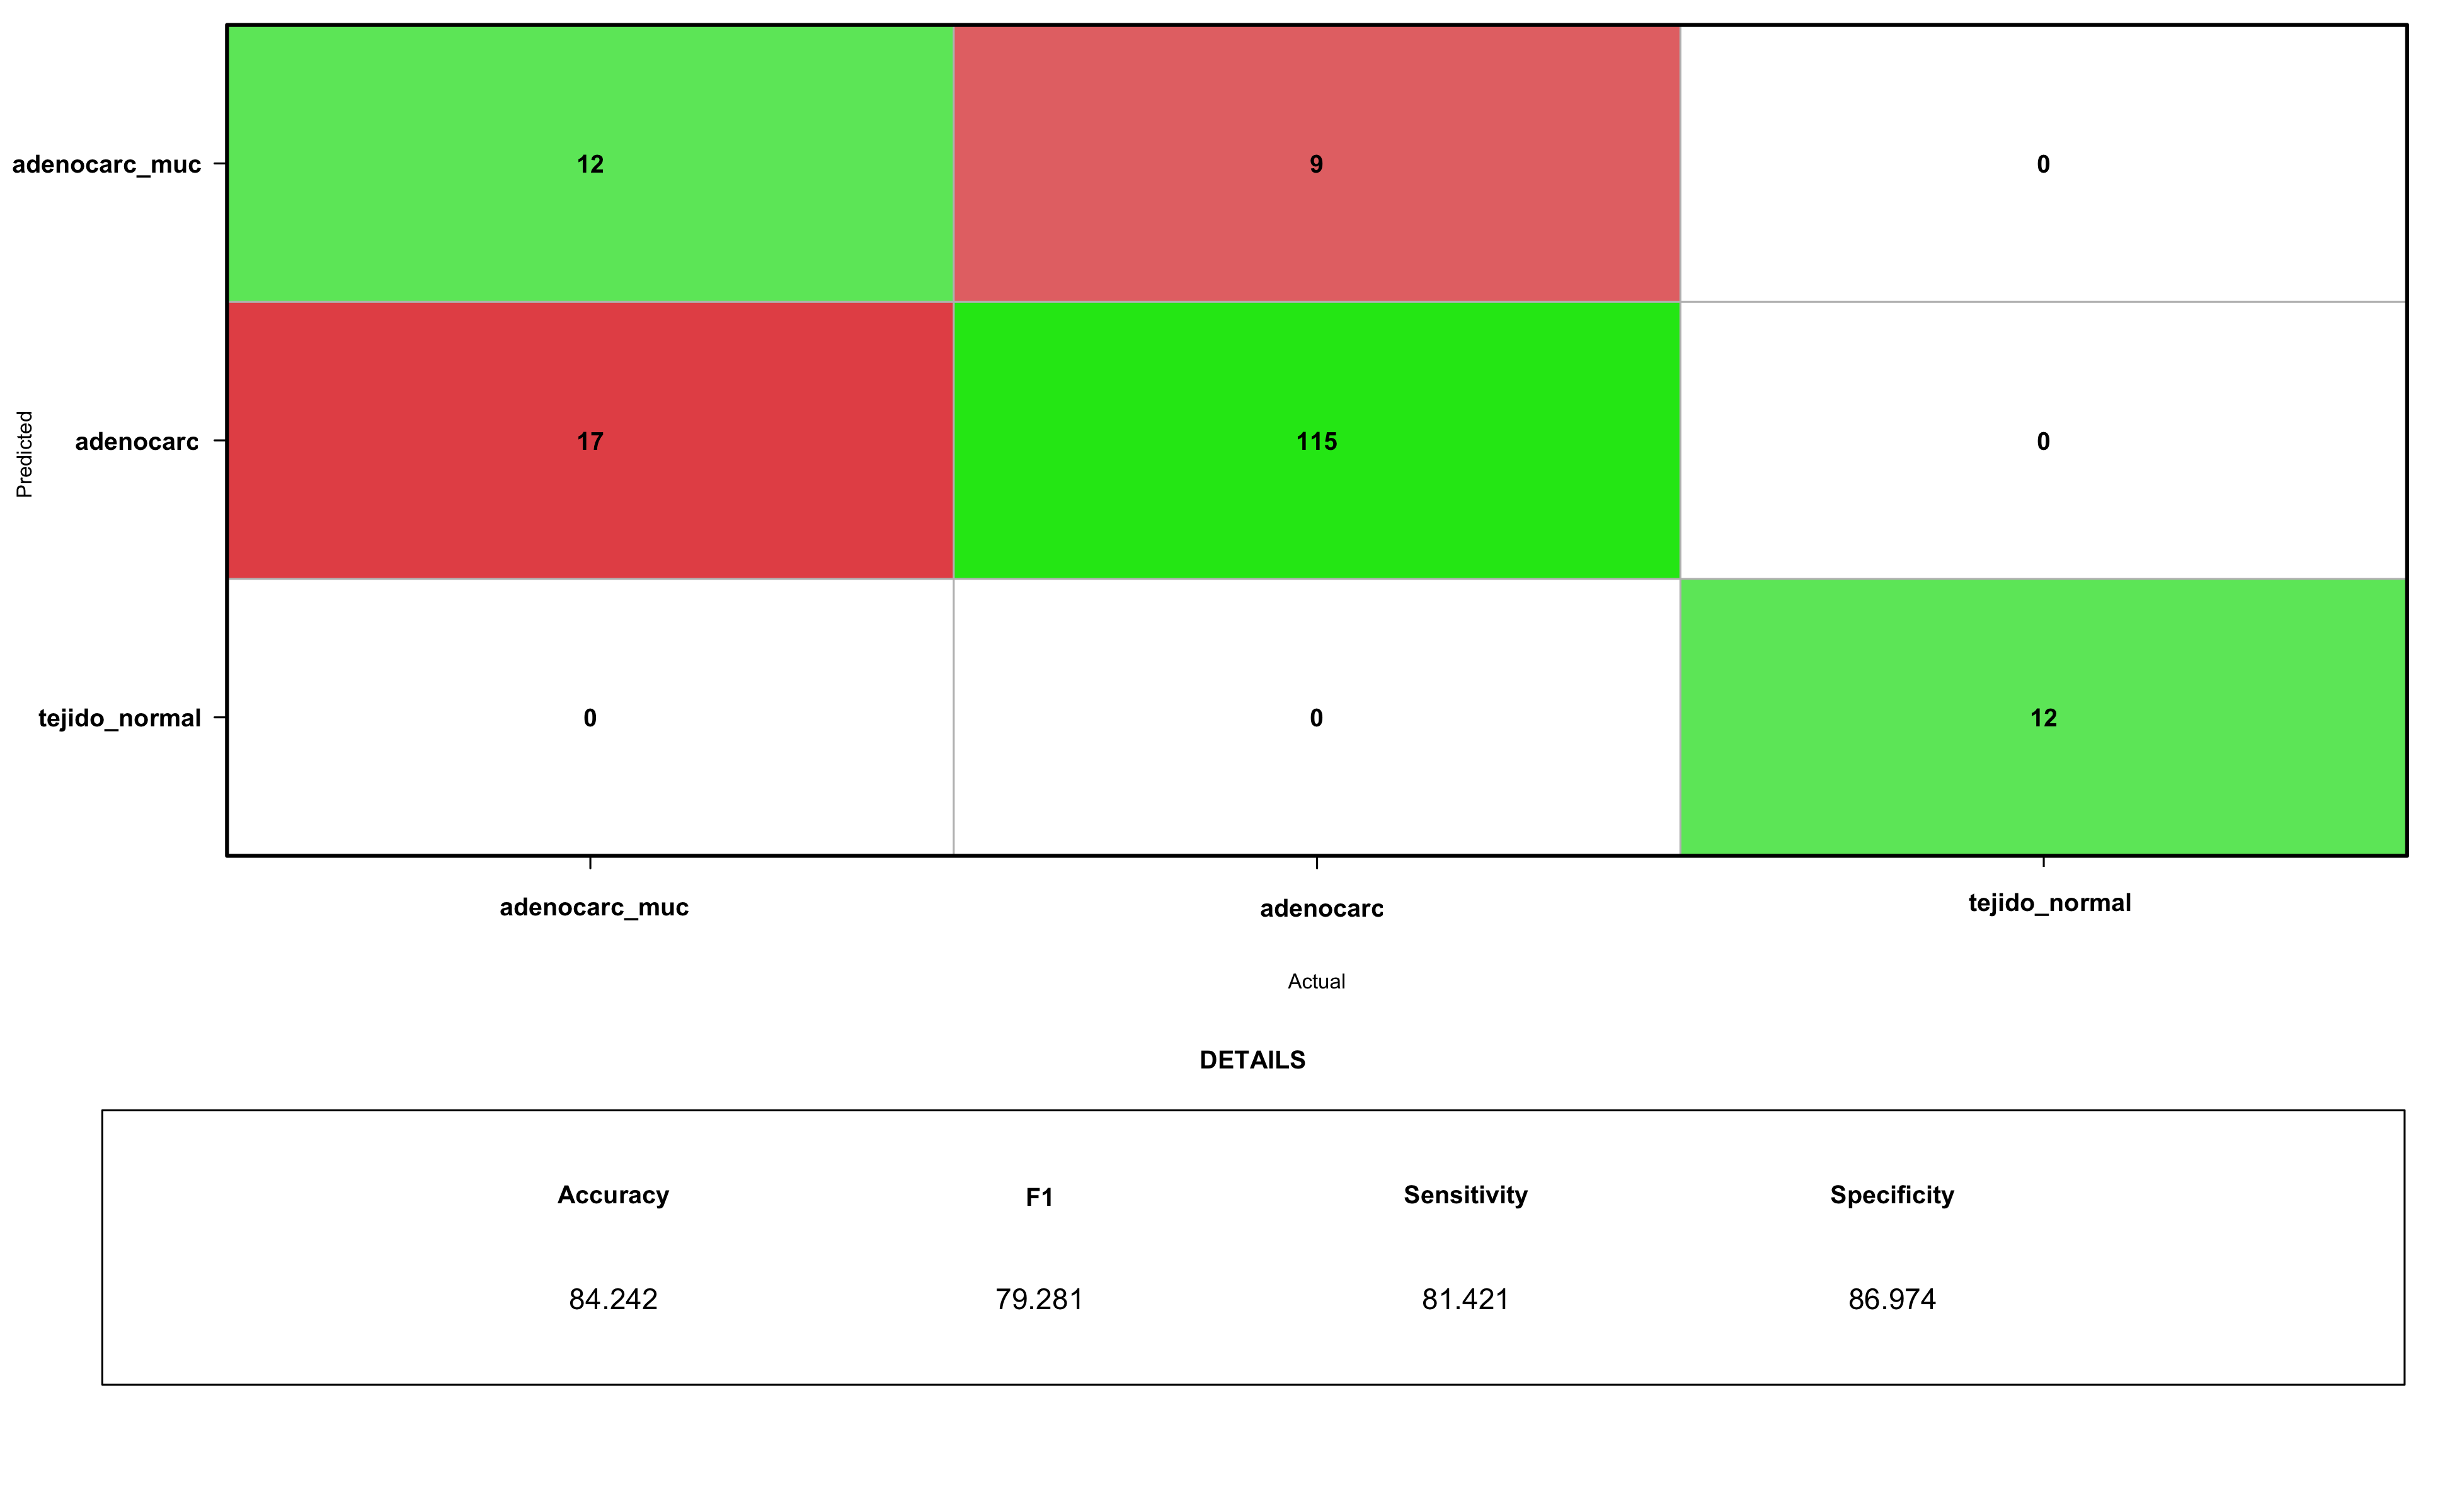
\includegraphics[width=1\textwidth]{figuras/40_cr_multiclase_25_rf_matriz_confusion_mejor_metodo.png} 
\end{center}

\newpage
\begin{center}
	\textbf{Figura 41}. Matriz de confusión del mejor modelo encontrado de kNN en el conjunto de test.
\end{center}

\begin{center}
	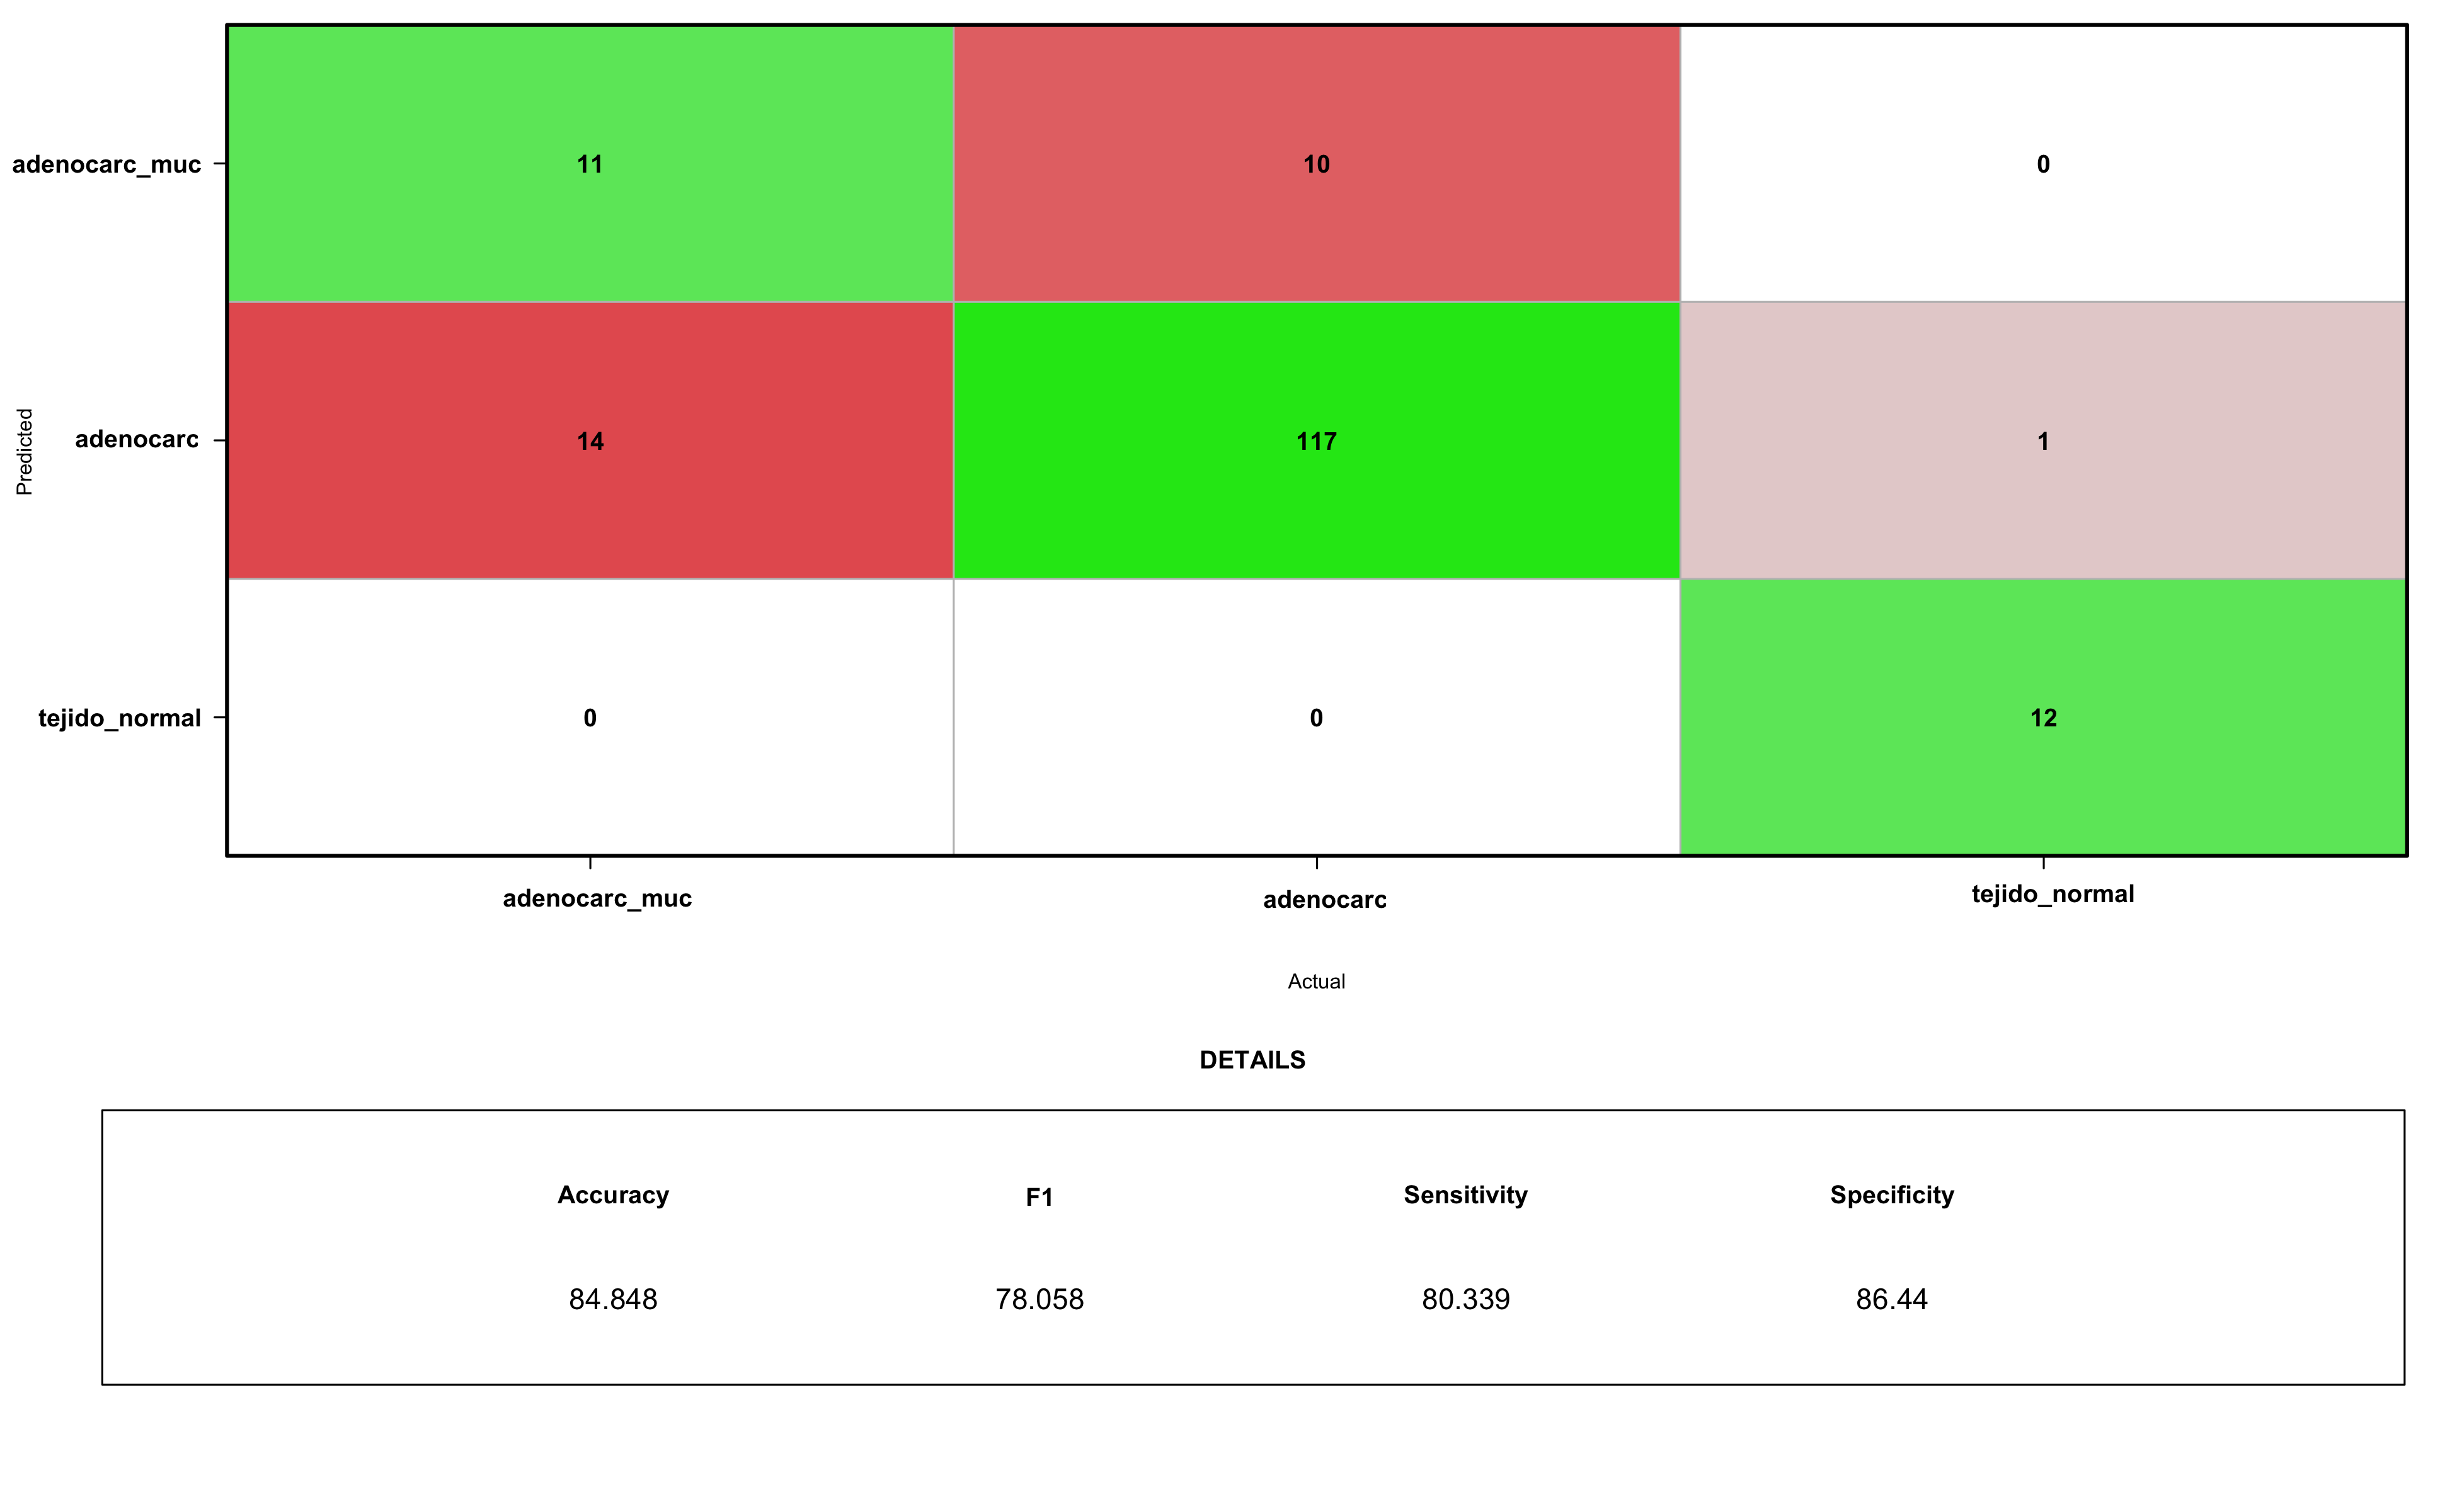
\includegraphics[width=1\textwidth]{figuras/41_cr_multiclase_35_knn_matriz_confusion_mejor_metodo.png} 
\end{center}

En la Tabla 37 se muestra un resumen de los mejores modelos obtenidos y su F1-Score y precisión en conjunto de entrenamiento y conjunto de test.\\

\textbf{Tabla 37}. Resumen de clasificación multiclase para cáncer de colon-recto. Mejor modelo encontrado para SVM, RF y kNN con biomarcadores seleccionados, parámetros optimizados para cada algoritmo, F1-Score y precisión (Acc) en conjunto de entrenamiento y conjunto de test.

\begin{table}[H]
	\centering
	\begin{tabular}{ccccc|cc}
		\cline{2-7}
		& Biomarcadores & Parámetros                                                        & F1 train & Acc train & F1 test & Acc test \\ \hline
		\multicolumn{1}{l}{SVM} & \textbf{3 genes} RF   & \begin{tabular}[c]{@{}c@{}}$c$ = 5\\ $\gamma$ = 0,07\end{tabular} & 81,61    & 90,25     & 80,29   & 87,27    \\
		RF                      &  \textbf{9 genes} mRMR  & --                                                                & 83,38    & 90,66     & 79,28   & 84,24    \\
		kNN                     & \textbf{3 genes} RF  & k = 7                                                             & 82,46    & 90,86     & 78,06   & 84,85    \\ \hline
	\end{tabular}
\end{table}

\subsection{Conclusiones}

En el caso de la clasificación multiclase para cáncer de colon-recto, los resultados son notablemente inferiores a los obtenidos en los otros problemas abordados en este trabajo. Se consigue una buena distinción entre tumores y sanos pero no así entre los diferentes tipos de tumores, algo que puede deberse a las pocas diferencias biológicas existentes entre adenocarcinomas y adenocarcinomas mucinosos. Los adenocarcinomas mucinosos son aquellos adenocarcinomas en los que se producen grandes cantidades de mucina (proteínas que produce el colon para ayudar a lubricación), y si este proceso de producción de mucina no se traduce en grandes diferencias en la expresión de los genes, es complicado distinguir los dos tipos de cáncer. \\

Se han analizado las enfermedades relacionadas con los mejores genes encontrados (3 genes con RF, 9 genes con mRMR) en la plataforma de Open Targets \cite{OpenTargets2020}. Se encuentra asociación entre todos los genes y el cáncer de colon-recto. Por ejemplo, el gen SLC11A1 está asociado con cáncer de colon-recto en múltiples referencias bibliográficas \cite{Law2019, Tanskanen2018, Huyghe2019}, así como con enfermedades intestinales inflamatorias \cite{Jostins2012, DeLange2017}. Genes relacionados con factores de riesgo de cáncer de colon-recto son OSBPL3 con consumo de tabaco \cite{Liu2019} y GTF2IRD1 con consumo de alcohol \cite{biobank}.

\section{Conclusiones finales}

Se presentan a continuación las conclusiones finales obtenidas tras analizar los distintos problemas de clasificación durante el presente Trabajo Fin de Máster.\\

Sobre los algoritmos de selección de características, mRMR y RF han demostrado ser buenos métodos, siempre mejores que DA, aunque carecen del enfoque médico en el que se basa este último método. Con menos de 10 genes se ha conseguido en general una buena clasificación, a menudo llegando a usar 2 ó 3 genes. Encontrar una técnica de clasificación adecuada con un número tan pequeño de genes puede suponer una mejora significativa en el pronóstico de pacientes con cáncer, ya que mediante técnicas simples de diagnóstico se pueden detectar tumores en estadios iniciales, lo que supone múltiples ventajas \cite{Whitaker2020}:

\begin{itemize}
	\item Mayor efectividad del tratamiento contra la enfermedad, y disminución de sus complicaciones y secuelas.
	\item Mejora de la calidad de vida del paciente.
	\item Aumento de la supervivencia.
\end{itemize}

Para considerar que existen una relación evidente gen-enfermedad es necesario contar con una interpretación clínica \cite{Drier2011}, no siendo suficiente una evidencia estadística. Este razonamiento  está en concordancia con el debate científico sobre el uso de p-valores en las últimas décadas \cite{Evans1988, Goodman1999, Matthews2000} y en la actualidad \cite{McShane2019, Wasserstein2019}. Por este motivo, sería interesante que expertos en el campo de investigación médica puedan analizar las huellas genéticas encontradas en el presente trabajo para poder establecer con claridad la relación gen-enfermedad cuando esta relación no está clara.\\

En general, los algoritmos de clasificación propuestos (SVM, RF y kNN) han obtenido resultados correctos y muy similares entre sí tanto para problemas biclase como multiclase. Una de las ventajas de trabajar con varios algoritmos de clasificación es que se puede escoger aquel que utiliza el menor número de genes, con las ventajas que ello conlleva (menor coste computacional y mayor interpretabilidad). Otra opción posible es escoger aquel algoritmo que aporte más interpretabilidad al problema (kNN en este caso). \\

Por último, sería interesante validar los excelentes resultados de los modelos encontrados en otros conjuntos de datos para probar la validez externa de los modelos \cite{Steckler2008}.\\